\documentclass{book}

\usepackage{graphicx}
\usepackage{multicol}
%\usepackage{multirow}
%\usepackage{bm} %% bold face math symbols
\usepackage{listings}
\usepackage{../macros/mytikz}
\usetikzlibrary{shapes}
%\usepackage{stmaryrd}%\newcommand{\contra}{\lightning}
%\usepackage{rotating} \newcommand{\sw}[1]{\begin{sideways}#1\end{sideways}}

\usepackage{../macros/algorithm}
%\usepackage{ded}
\usepackage{../mylecturenotes}
\usepackage{../macros}

\title{Lectures Notes on Secure and Dependable Systems}
\author{Florian Rabe}
\date{2017}


\begin{document}
\maketitle

\tableofcontents
\newpage

\part{Introduction}

 \chapter{Meta-Remarks}
  \input{../generalremarks}

  \chapter{Concepts}
   \section{Abbreviations}

\begin{center}
\begin{tabular}{lll}
knowledge representation and processing & KRP & the general area of this course \\
knowledge representation language & KRL & a languages used in KRP \\
knowledge representation tool & KRT & a tool implementing a KPL and processing algorithms for it
\end{tabular}
\end{center}

\section{Motivation}

\subsection{Knowledge}

Human knowledge pervades all sciences including computer science, mathematics, natural sciences and engineering.
That is not surprising: \enquote{science} is derived from the Latin word \enquote{scire} meaning \enquote{to know}.
Similarly, philosophy, from which all sciences derive, is named after the Greek words \enquote{philo} meaning loving and \enquote{sophia} meaning wisdom, and the common ending \enquote{-logy} is derived from Greek \enquote{logos} meaning word (i.\,e., a representation of knowledge).

In regards to knowledge, computer science is special in two ways:
Firstly, many branches of computer science need to understand KRP as a prerequisite for teaching computers to do knowledge-based tasks.
In some sense, KRP is the foundation and ultimate goal of all artificial intelligence.%
\footnote{Indeed, a major problem with the currently very successful machine learning-based AI technology is that it remains unclear when and how it does KRP. That can be dangerous because it leads to AI systems recommending decisions without being able to explain why that decision should be trusted.}
Secondly, modern information technology enables all sciences to apply computer-based KRP in order to vastly expand on the domain-specific tasks that can be automated.
Currently all sciences are becoming more and more computerized, but most non-CS scientists (and many computer scientists for that matter) lack a systematic education and understanding of IT-KRP.
That often leads to bad solutions when domain experts cannot see which KRP solutions are applicable or how to apply them.

\subsection{Representation and Processing}

It is no coincidence that this course uses the phrase \enquote{Representation and Processing}.
In fact, this is an instance of a universal duality.
Consider the following table of analogous concept pairs, which could be extended with many more examples:

\begin{center}
\begin{tabular}{ll}
\toprule
Representation & Processing \\
\midrule
Static & Dynamic \\
Situation & Change \\
Be & Become \\
Data Structures & Algorithms \\
Set & Function \\
State & Transition \\
Space & Time \\
\bottomrule
\end{tabular}
\end{center}

Again and again, we distinguish a static concept that describes/represents what a situation/state is and a dynamic concept that describes how it changes.
If that change is a computer doing something with or acting on that representation, we speak of \enquote{processing}.

It is particular illuminating to contrast KRP to the standard CS course on Data Structures and Algorithms (DA).%
\footnote{The course is typically called \enquote{Algorithms and Data Structures}, but that is arguably awkward because algorithms can only exist if there are data structure to work with. Compare my notes on that course in this repository, where I emphasize data structures much more than is commonly done in that course.}
Generally speaking, DA teaches the methods, and KRP teaches how to apply them.
Data structures are a critical prerequisite for representing knowledge.
But data structures alone do not capture what the data means (i.\,e., the knowledge) or if a particular representation makes any sense.
Similarly, algorithms are the critical prerequisite for processing knowledge.
But while algorithms can be systematically analyzed for efficiency, it is much harder to analyze if an algorithm processes knowledge correctly.
The latter requires understanding what the input and output data means.

Capturing knowledge in computers is much harder than developing data structures and algorithms.
It is ultimately the same challenge as figuring out if a computer system is working correctly --- a problem that is well-known to be undecidable in general and very difficult in each individual case.

%%%%%%%%%%%%%%%%%%%%%%%%%%%%%%%%%%%%%%%%%%%%%%%%%%%%%%%%%%%%%%%
\section{Components of Knowledge}

\subsection{Syntax and Semantics, Data and Knowledge}

Four concepts are of particular relevance to understanding knowledge.
They form a $2\times 2$-quadruple of concepts:

\begin{center}
\begin{tabular}{l|l}
Syntax & Data \\
\hline
Semantics & Knowledge
\end{tabular}
\end{center}

All four concepts are primitive, i.\,e., they cannot be defined in simpler terms.
All sciences have few carefully-chosen primitives on which everything builds.
This is done most systematically in mathematics (where primitives include set or function).
While mathematical primitives as well as some primitives in physics or CS are specified formally, the above four concepts can only be described informally, ultimately appealing to pre-existing human understanding.
Moreover, this description is not standardized --- different courses may use very different descriptions even if they ultimately try to capture the same elusive ideas.

\textbf{Data} (in the narrow sense of computer science) is any object that can be stored in a computer, typically combined with the ability to input/output, transfer, and change the object.
This includes bits, strings, numbers, files, etc.

Data by itself is useless because we would have no idea what to do with it.
For example, the object $O=((49.5739143, 11.0264941), "2020-04-21\text{T}16:15:00\text{CEST}")$ is useless data without additional information about its syntax and semantics.
Similarly, a file is useless data unless we know which file format it uses.

\textbf{Syntax} is a system of rules that describes which data is \textbf{well-formed}.
For $O$ above the syntax could be \enquote{a pair of (a pair of two IEEE double precision floating point numbers) and a string encoding of an time stamp}. 
For a file, the syntax is often indicated by the file name extension, e.\,g., the syntax of an \texttt{html} file is given in Section 12 of the current HTML standard\footnote{\url{https://html.spec.whatwg.org/multipage/}}.

Syntax alone is useless unless we know what the semantics, i.\,e., what the data means and thus how to correctly interpret and process the data.
For example, the syntax of $O$ allows to check that $O$ is well-formed, i.\,e., indeed contains two numbers and a timestamp string.
That allows rejecting ill-formed data such as $((49.5739143, 11.0264941), "\text{foo}")$.
The HTML syntax allows us to check that a file conforms to the standard.

\textbf{Semantics} is a system of rules that determines the meaning of well-formed data.
For example, ISO 8601 specifies that timestamp string refer to a particular date and time in a particular time zone.
Further semantics for $O$ might be implicit in the algorithms that produce and consume it: such as \enquote{the first component of the pair contains two numbers between $0$ and $180$ resp. $0$ and $360$ indicating latitude resp. longitude of a location on earth}.
Semantics might be multi-staged, and further semantics about $O$ might be that $O$ indicates the location and time of the first lecture of this course.
Similarly, Section 14 of the HTML standard specifies the semantics of well-formed HTML files by describing how they are to be rendered in a web browser.

\textbf{Knowledge} is the combining of some data with its syntax and semantics.
That allows applying the semantics to obtain the meaning of the data (if syntactically well-formed and signaling an error otherwise).
In computer systems,
\begin{compactitem}
 \item data is represented using primitive data (ultimately the bits provided by the hardware) and encodings of more complex data (bytes, arrays, strings, etc.) in terms of simpler ones,
 \item syntax is theoretically specified using grammars and practically implemented in programming languages using data structures,
 \item semantics is represented using algorithms that process syntactically well-formed data,
 \item knowledge is elusive and often emerges from executing the semantics, e.\,g., rendering of an HTML file.
\end{compactitem}

\subsection{Semantics as Syntax Transformation}

In order to capture knowledge better in computer systems, we often use two syntax levels: one to represent the data itself and another to represent the knowledge.
These can be seen as input and output data.
In that case, semantics is a function that translates from the data syntax to the knowledge syntax, and knowledge is the pair of the data and the result of applying the semantics.
The following table gives some examples.

\begin{center}
\begin{tabular}{lll}
\toprule
Data syntax & Semantics function & Knowledge syntax \\
\midrule
SPARQL query & evaluation & result set \\
SQL query & evaluation & result table \\
program & compiler & binary code \\
program expression & interpreter & result value \\ 
logical formula & interpretation in a model & mathematical object \\
HTML document & rendering & graphical representation \\
\bottomrule
\end{tabular}
\end{center}

Thus, the role of syntax vs.\ semantics may depend on the context: just like one function's output can be another function's input, one interpretation's knowledge can be another one's syntax.
For example, we can first compile a program into binary and then execute it to returns its value.

Such hierarchies of evaluation levels are very common in computer systems.
In fact, most state-of-the-art compilers are subdivided into multiple phases each further interpreting the output of the previous one.
Thus, if knowledge is represented in computers, it is invariably data itself but relative to a different syntax.

\subsection{Heterogeneity of Semantics and Knowledge}

While it is easy to design languages to represent data in general, it is very difficult to designing KRLs that capture the human-level quality of knowledge.
Over the last few decades, the KRP area in computer science has diversified into different subareas that approach this research problem in fundamentally different ways.
In fact, KRP in the very general sense of this course is usually not even studied by itself --- instead the subareas are so different, specialized, and large that they all sustain their respective university courses and research conferences.

This is related to the fact that the data naturally comes in fundamentally different forms such as graphs, arrays, tables in the sense of relational databases, programs in a programming language, logical formulas, or natural language texts.
We speak of \textbf{heterogeneous} data.
These different forms of data are supported by highly specialized KPTs: graph databases, array databases, relational databases, package databases for programming languages, theorem databases for logics (e.\,g., the Isabelle Archive of Formal Proofs), databases of research papers (such as the arXiv), and so on.

All of these are very successful for their respective kind of data.
And all of them include specifications of semantics and KP algorithms that implement this semantics.
But it can vary massively how the semantics is specified and implemented.
This has caused major practical problems for tool interoperability: many projects require data in multiple formats and algorithms from multiple tools.
But the respective tools are often islands that assume that all data is represented in the tool's language and users do not use outside tools.
Therefore, the import/export capabilities of the tools are often limited.

Moreover, transporting data across systems is usually ignorant of the semantics: while each tool takes relatively good care to implement the semantics correctly, there is much less certainty that the semantics is preserved when exchanging data across tools.
For a trivial example, consider a tool that measures length in inches vs.\ a tool that uses centimeters, both using floating point numbers for the data: if they exchange the data, i.\,e., just the numbers, they may miscommunicate the semantics.%
\footnote{Problems like this have been involved in major disasters such as the Mars Climate Orbiter.} 

This problem is not easy to fix though.
The heterogeneity of data and semantics is so extreme that it is, in some cases, an open theoretical problem how knowledge can be shared at all across tools.
The basic idea --- exchange the data in a way that preserves semantics --- can be difficult to implement if both tools use entirely different paradigms to specify semantics.

%%%%%%%%%%%%%%%%%%%%%%%%%%%%%%%%%%%%%%%%%%%%%%%%%%%%%%%%%%%%%%%
\section{The Tetrapod Model of Knowledge}

The Tetrapod model of knowledge is an ongoing research project by the instructors of this course.
A first publication was made in \cite{CFKR:tetrapod:19}.
The structure of this course will draw heavily on the Tetrapod model to get an overview of the different approaches to KPR and their interoperability problems.

\subsection{Five Aspects of Knowledge}

The Tetrapod model distinguishes five basic \textbf{aspects} of knowledge and KPR as described below.
For each aspect, there is a variety dedicated KRLs supported by highly optimized KPTs as indicated in the following table:

\begin{center}
\begin{tabular}{lll}
\toprule
Aspect & KRLs (examples) & KPTs (examples) \\
\midrule
ontologization & ontology languages (OWL), description logics (ALC) & reasoners, SPARQL engines (Virtuoso) \\
concretization & relational databases (SQL, JSON) & databases (MySQL, MongoDb) \\
computation & programming languages (C) & interpreters, compilers (gcc) \\
deduction & logics (HOL) & theorem provers (Isabelle) \\
narration & document languages (HTML, LaTeX) & editors, viewers \\
\bottomrule
\end{tabular}
\end{center}

\textbf{Ontologization} focuses on developing and curating a coherent and comprehensive ontology of concepts.
This focuses on identifying the central concepts in a domain and their relations.
For example, a medical ontology would define concepts for every symptom, disease, and medication and then define relations for which symptoms and medications are related to which disease.

Ontologies typically abstract from the knowledge: they standardize identifiers for the concepts and spell out some properties and relations but do not try to capture all details of the knowledge.
Well-designed ontologies can capture exactly what different KPTs must share and can thus serve as interoperability layers between them.

While organization can use ontology languages such as OWL or RDF, the inherent complexity of formal objects in computer science and mathematics usually requires going beyond general purpose ontology languages (similar to how the programming languages underlying computer algebra systems usually go beyond general purpose programming languages).

\textbf{Concretization} uses languages based on numbers, strings, lists, and records to obtain concrete representations of datasets in order to store and query their properties efficiently.
Because concrete objects are so simple and widely used, it is possible and common to build concrete datasets on top of general purpose data representation languages and tools such as JSON or SQL.

\textbf{Computation} uses specification and programming languages to represent algorithmic knowledge.

\textbf{Deduction} uses logics and theorem provers  to obtain verifiable correctness.

\textbf{Narration} uses natural language to obtain texts that are easy to understand for humans.
Because narrative languages are not well-standardized (apart from general purpose languages such as free text or \LaTeX), it is common to develop narrative libraries on top of ad-hoc languages that impose some formal structure on top of informal text, such as a fixed tree structure whose leafs are free text or a particular set of {\LaTeX} macros that must be used.
Narrative libraries can be classified based on whether entries are derived from publications (e.\,g., one abstract per paper in zbMATH) or mathematical concepts (e.\,g., one page per concept in $n$Lab).
%While these languages have multiple implementations, individual libraries usually involve specific encodings that are implemented only by a single tool.

%For example, an organization language might state only a function's type and properties.
%A computational treatment provides an efficient implementation, a deductive one proves the properties, a concretized one tables the function's values, and a narrative one documents the nature and purpose of the function.


\subsection{Relations between the Aspects}

The aspects can be visualized as the corners of tetrahedron with ontologization in the center and edges and faces representing solutions that mix two or three aspects as seen in Figure~\ref{fig:tetrapod}.

\begin{figure}[hbt]
\begin{center}
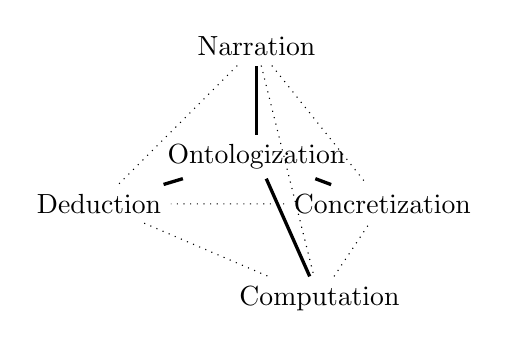
\begin{tikzpicture}[scale=4]
  \node (center) at (0,.15) {Ontologization};
  \node (left) at (.2,-.3) {Computation};
  \node (right) at (.4,0) {Concretization};
  \node (back) at (-.5,0) {Deduction};
  \node (up) at (0,.5) {Narration};

  \draw[very thick] (center) -- (left);
  \draw[very thick] (center) -- (right);
  \draw[very thick] (center) -- (back);
  \draw[very thick] (center) -- (up);
  \draw[dotted] (left) -- (right) -- (back) -- (left);
  \draw[dotted] (up) -- (left);
  \draw[dotted] (up) -- (right);
  \draw[dotted] (up) -- (back);
\end{tikzpicture}
\end{center}
\caption{Tetrapod model of knowledge}\label{fig:tetrapod}
\end{figure}

Most approaches try to incorporate all or multiple aspects.
But all languages and tools tend to be heavily biased towards and optimized for a single one of the four corner aspects.
This is not due to ignorance but because each aspect provides characteristic advantages that are extremely hard to capture at once.
In fact, every combination of aspects shares characteristic advantages and disadvantages as sketched in~\autoref{fig:tetrapod2}.
For example, deductive and narrative definitions of a function involved well-definedness arguments, and a function defined by a concrete table is trivially well-defined, but a computational definition of a function may throw exceptions when running; but only the latter can store and compute functions efficiently.
Consequently, dedicated and mostly disjoint communities have evolved that have produced large aspect-specific datasets.

\begin{table}[h]
\caption{Shared properties and advantages of aspects}\label{fig:tetrapod2}
\begin{subtable}{\textwidth}
\centering
\caption{Characteristics of aspects}
\begin{tabular}{lllp{2.8cm}l}
\toprule
	& \multicolumn{4}{c}{characteristic} \\
\cmidrule(lr){2-5}
Aspect &  objects & advantage & joint advantage of the other aspects & application \\
\midrule
deduction & formal proofs & correctness & ease of use & verification \\
computation & programs & efficiency & well-definedness & execution\\
concretization & concrete objects & tangibility & abstraction & storage/retrieval\\
narration & texts & flexibility & formal semantics & human understanding\\
\bottomrule
\end{tabular}
\end{subtable}

\medskip
\begin{subtable}{\textwidth}
\centering
\caption{Advantages of aspect pairs}
\begin{tabular}{ll}
\toprule
Aspect pair & characteristic advantage \\
\midrule
deduction/computation  & rich meta-theory \\
narration/concretization & simple languages \\
\addlinespace
deduction/narration  & theorems and proofs \\
computation/concretization & normalization \\
\addlinespace
deduction/concretization  & decidable well-definedness \\
computation/narration & Turing completeness \\
\bottomrule
\end{tabular}
\end{subtable}
\end{table}

%\subsection{Aspect-Specific Datasets in Mathematics}
%
%A survey of the state of the art in aspects is huge.
%Figure~\ref{fig:libraries} gives an overview of important datasets just the domain of mathematics.
%We have also pre-published a draft of an extensive survey in \cite{CarFarSharBerKohMueRab:somss20}.
%
%Crucially, these disjoint projects overlap massively.
%For example, the concept of \emph{group} is defined in most proof assistants and computer algebra systems, concrete groups are part of multiple large libraries (e.\,g., as the main object of interest in the small groups libraries, or as symmetry groups arising from other objects), and has entries in most narrative libraries (e.\,g., with entries in Stacks and nLab).
%Despite the overwhelming practical need, at the moment there is little to no technology to integrate libraries across this overlap.
%The same effect is found in other domains.
%
%\begin{figure}[ht]\centering\small\def\cite#1{}
%  \begin{tabular}{| p{.3\textwidth} | p{0.55\textwidth}|}\hline
%  Dataset & Description and approximate size \\\hline\hline
%  \multicolumn{2}{|l|}{\textbf{Inference}} \\\hline
%  Theorem prover libraries  & ??? \\\hline
%  \multicolumn{2}{|l|}{\textbf{Computation} \hfill\strut\hfill {\tiny CAS = computer algebra system}} \\\hline
%  Mathematica & commercial CAS, $5k$ built-in functions, $150$k official examples\\\hline
%  Maple & commercial CAS, $5$k built-in functions \\\hline
%  GAP \cite{gap} & CAS for group theory, $10$k statements \\\hline
%  Singular \cite{singular:on} & CAS for polynomials, over $90$ libraries \\\hline
%  SageMath \cite{SageMath:on} & $1$k modules, bundled with $4$GB of CAS tools and libraries\\\hline
%  Modelica \cite{Modelica:on} & modeling language, $5$k built-in classes, $100$ open source libraries, $50$ commercial libraries up to $0.5$M equations \\\hline\hline % $10$ official, $>100$ open-source, $50$ commercial,
%  \multicolumn{2}{|l|}{\textbf{Concretization}} \\\hline
% OEIS \cite{OEIS:on} & $330$k integer sequences, $1$ TB; $0.3$M sequence identities in \cite{kwarc:datahost:on} \\\hline
%%  OEIS identities \cite{kwarc:datahost:on} & $0.3$M sequence identities, $2.5$ TB \\\hline
% various databases of graphs\cite{ConderCensuses:on, HartleyPolytopes:on, LeemansPolytopes:on, PotocnikCensuses:on, RoyleVT:on, WilsonET:on} & highly symmetric graphs, maps, polytopes, $30$ datasets, $2$M objects, $1$TB \\\hline
%  various databases of lattices \cite{KohLat:on, LeeLat:on, MalLat:on} & $7$ datasets, $17$G objects, $1.5$ TB \\\hline
%  findstat \cite{findstat} & combinatorial statistics and maps, $1.5$k objects \\\hline
%  SageMath databases \cite{SageDB:on} & $12$ datasets \\\hline
%  $L$-functions and modular forms \cite{lmfdb:on} & $80$ datasets, $1$G objects, $1$ TB \\\hline
%  Small Groups Library \cite{BeEiOBSmallGroups} & $450$M groups, $80$ MB \\\hline\hline
%  \multicolumn{2}{|l|}{\textbf{Narration}\hfill\strut\hfill {\tiny based on publications (P) or concepts (C)}} \\\hline
%  arXiv.org (P) & $300$k math preprints, most with {\LaTeX} sources\\\hline
%  zbMATH \cite{zbMATH:on} (P) & $4$M publication abstracts with semantic data, $30$M reference data, $1$M disambig. authors, $2.7$M full text links \\\hline % $1$M OA 
%  EuDML  \cite{EuDML:on} (P) & $260$k open full-text publications, digitized journal back issues \\\hline
%%  MathOverFlow & $\approx 1,1$M questions/answers, $\geq11$K answer authors \\\hline
%  Stacks project (C) & $6$k pages, semantically annotated, curated, searchable textbook \\\hline
%  $n$Lab (C) & $13$k pages on category theory and applications\\\hline
%  SMGloM glossary (C) & $1$k modules, $2$k concepts, $4.5$k multi-lingual verbalizations in English \\\hline\hline %  (100\%), German (90\%), Chinese (10\%)
%  \multicolumn{2}{|l|}{\textbf{Organization}} \\\hline
%  swMATH \cite{swMATH:on} & $25$k software records with $300$k links to $180$k publications \\\hline
%  Wikidata  \cite{wikidata:on} & $34$GB linked data, $4$k formulas, interlinked with named theorems, persons, publications \\\hline
%  DLMF & $500$ special mathematical functions, $10$k formulas \\\hline
%  OpenMath CDs \cite{openmath} & curated reference points for $1.5$k concepts \\\hline
%  LATIN atlas \cite{CHKMR:latinabs:11,LATIN:online} & modular definitions of logics, $1$k modules \\\hline
%  Formal Abstracts  \cite{fabstracts} & formal definitions for all concepts used by multiple authors of mathematical papers (planned) \\\hline
%  \oaf interface library & as obtained in \oaf WP 2.6\\\hline
%\end{tabular}
%  \caption{Representative examples of large libraries by aspect}\label{fig:libraries}
%\end{figure}


 \chapter{Challenges}
   This chapter lists examples of disasters and failures that serve as examples of what secure and dependable systems should avoid.

The lists are not complete and may be biased by whether
\begin{compactitem}
 \item I became aware of it and found it interesting enough
 \item the cause could be determined and was made public
\end{compactitem}
Feel free to edit these notes by adding important examples that I forgot when I compiled the lists.

All damage estimates are relative to the time of the event and not adjusted to inflation.

Note that for security problems, the size of the damage is naturally unknown because attacks will typically remain secret.
Only the cost of updating the systems can be estimated, which may or may not be indicative of the severity of the security problem.

\section{General Aspects}

\highlightframe{
State-of-the-art software and hardware systems simply are not safe, secure, and dependable.

Moreover, we do not understand very well yet how to make them so.
}

This is different from many other areas such as mechanical or chemical engineering.
While these occasionally cause disasters, these can usually be traced back to human error, foul play, or negligent or intentional violation of regulations.
Such disasters usually result in criminal proceedings, civil litigation, or revision or extension of regulations.
% what engineers know and how they know it

The situation is very different for computer systems.
There is no general methodology for designing and operating computer systems well that can be easily described, taught, or codified.

The situation will hopefully improve over the course of the 21st century.
The problem has been recognized decades ago, and many companies and researchers are working on it.
They approach from very different directions with different goals and different methodologies.

\highlightframe{
This has resulted in a wide and diverse variety of not coherently connected methods with varying degrees of depth, maturity, cost, benefit, and practical adoption.
}

A typical effect is a trade-off along a spectrum of methods:
\begin{compactitem}
 \item cheap but weak methods on one end
 \item strong but expensive methods on the other end.
\end{compactitem}
Therefore, it is often necessary to choose a degree of safety assurance rather than actually guarantee safety.
This spectrum is so extreme that
\begin{compactitem}
 \item the majority of practical software development does not systematically ensure any kind of safety,
 \item the majority of theoretical solutions are neither ready nor affordable for practical use.
\end{compactitem}

Incidentally, this means that this course's subject matter is much less well-defined than that of other courses.%
\footnote{For example, the other two courses in this module almost design themselves because the subject matter is very well understood and standardized.}
That makes it particular difficult to design a syllabus for.
It will give an overview of the most important state-of-the-art methods.

\section{Major Disasters Caused by Programming Errors}

\paragraph{Space Exploration}
There have been a number of failures in space exploration due to minor programming errors.
These include
\begin{compactitem}
 \item 1962, Mariner 1 rocket lost: misread specification (overlooked bar over a variable) was implemented (damage around \$$20$ million)
 \item 1982, Viking I lost: software update written to wrong memory area overriding vital parameters for antenna
 \item 1988, Phobos 1 lost: one character missing in software update led to accidentally executing a testing routine at the wrong time
 \item 1996, Mars Global Surveyor lost: data written to wrong memory addresses
 \item 1999, Mars Polar Lander lost: presumably software not accounting for false positive when detecting shutdown even though the possibility was known
 \item 2004, Mars Rover Spirit lost for 16 days: delay in deleting obsolete files led to lack of available flash memory, which triggered a reboot, which led to a reboot cycle
\end{compactitem}
% the story of a Fortran bug where . was accidentally written instead of a , appears to be exaaggerated; it did not lead to a crash

\paragraph{Therac-25}
Between 1985 and 1987, the Therac-25 machine for medical radiation therapy caused death and/or serious injury in at least $6$ cases.
Patients received a radiation overdose because the high intensity energy beam was administered while using the protection meant for the low intensity beam.

The cause was that the hardware protection was discontinued, relying exclusively on software to prevent a mismatch of beam and protection configuration.
But the software had always been buggy due to systemic failures in the software engineering process including complex systems (code written in assembly, machine had its own OS), lack of software review, insufficient testing (overall system could not be tested), bad documentation (error codes were not documented), and bad user interface (critical safety errors could be overridden manually, thus effectively being warnings).

Details: \url{https://en.wikipedia.org/wiki/Therac-25}

\paragraph{Patriot Rounding Error}
In 1991 during the Gulf war, a US Patriot anti-missile battery failed to track an incoming Iraqi Scud missile resulting the death of 28 people.

The cause was a rounding error in the floating point computation used for analyzing the missile's path.
The software had to divide a large integer (number of $0.1s$ clock cycles since boot $100$ hours ago) by $10$ to obtain the time in seconds.
This was done using a floating-point multiplication by $0.1$ --- but $0.1$ is off by around $0.000000095$ when chopped to a $24$-bits binary float.
The resulting time was off by $0.3$ seconds, which, combined with the high speed of the Scud missile, led to a serious miscalculation of the flight path.

Details: \url{http://www-users.math.umn.edu/~arnold/disasters/patriot.html}

\paragraph{Ariane 5}
In 1996, the first launch of an Ariane 5 rocket (at a cost of over \$$300$ million for rocket and payload) failed, and the rocket had to be destroyed after launch.
Both the primary and the backup system had shut down, each trying to transfer control to the other after encountering the same behavior, which they falsely interpreted as a hardware error.

The cause was an overflow exception in the alignment system caused by converting a $64$-bit float to a $16$-bit integer, which was not caught and resulted in the display of diagnostic data that the autopilot could not interpret.
The programmers were aware of the problem but had falsely concluded that no conversion check was needed (and therefore omitted the check to speed up processing).
Their conclusion had been made based on Ariane 4 flight data that turned out to be inappropriate for Ariane 5.

The faulty component was not even needed for flight and was only kept active for a brief time after launch for convenience and in order to avoid changing a running system.

Details: \url{http://www-users.math.umn.edu/~arnold/disasters/ariane5rep.html}

\paragraph{Intel Pentium Bug}
In 1994, it was discovered that the Intel Pentium processor (at the time widely used in desktop computers) wrongly computed certain floating point divisions.
The cost of replacing the CPUs was estimated at about \$$400$ million.

The error occurred in about 1 in 9 billion divisions.
For example, $4195835.0/3145727.0$ yielded $1.333 739 068 902 037 589$ instead of $1.333 820 449 136 241 000$.

The cause was a bug in the design of the floating point unit's circuit.

\paragraph{Kerberos Random Number Generator}
From 1988 to 1996, the network authentication protocol Kerberos used a mis-designed random number generation algorithm.
The resulting keys were so predictable that brute force attacks became trivial although it is unclear if the bug was ever exploited.

The cause was the lack of a truly random seed value for the algorithm.
Moreover, the error persisted across attempted fixes because of process failures (code hard to read, programmers had moved on to next version).

Detail: \url{http://docs.lib.purdue.edu/cgi/viewcontent.cgi?article=2331&context=cstech}

\paragraph{USS Yorktown}
In 1997, critical navigation and weapons hardware on the USS Yorktown was paralyzed at sea for $3$ hours while rebooting machines.

The cause was a blank field in a database that was interpreted as $0$ leading to a division-by-zero.
Special floating point values such as infinity or NaN were not used, thus resulting in an exception.
The exception was handled by neither the software nor the operating systems (Windows NT) thus crashing both.

Details: \url{http://www.cs.berkeley.edu/~wkahan/Boulder.pdf}

\paragraph{Mars Climate Orbiter}
In 1998 the Mars Climate Orbiter was lost causing damage of around \$$300$ million after software had calculated a false trajectory when updating the position of the spacecraft.

The cause was that two components by different manufacturers exchanged physical quantities as plain numbers (i.e., without units).
One component assumed customary units (pound seconds) whereas the other assumed SI units (Newton seconds).
The first component was in violation of the specification of the interface.

\paragraph{Year 2000 and 2038 Problems}
Leading to the year 2000, about \$$300$ billion were spent worldwide to update outdated software that was unable to handle dates with a year of $2000$ or higher.

The cause was that much software was used far beyond the originally envisioned lifetime.
At programming time, especially at times when memory was still scarce, it made sense to use only two digits for the year in a date.
That assumption became flawed when dates over $2000$ had to be handled.

A related problem is expected in the year 2038.
At that point the number of seconds since 1970-01-01, which is the dominant way of storing time on Unix, will exceed the capacity of a $32$-bit integer.
While application software is expected to be updated by then anyway, modern embedded systems may or may not still be in use.

\paragraph{Los Angeles Airport Network Outage}
In 2007, LA airport was partially blocked for $10$ hours due to a network outage that prevented passenger processing.
About 17,000 passengers were affected.

The cause was a single network card malfunction that flooded the network and propagated through the local area network.

Details: \url{https://www.oig.dhs.gov/assets/Mgmt/OIGr_08-58_May08.pdf}

\paragraph{Debian OpenSSL Random Number Generator}
From 2006 to 2008 Debian's variant of OpenSSL used a flawed random number generator.
This made the generated keys easily predictable and thus compromised.
It is unclear whether this was exploited.

The cause was that two values were used to obtain random input: the process ID and an uninitialized memory field.
Uninitialized memory should never be used but is sometimes used as a convenient way to cheaply obtain a random number in a low-level programming language like C.
The respective line of code had no immediately obvious purpose because it was not commented.
Therefore, it was removed by one contributor after code analysis tools had detected the use of uninitialized memory and flagged it as a potential bug.

Detail: \url{https://github.com/g0tmi1k/debian-ssh}

\paragraph{Knight Capital Trading Software}
In 2012, high-frequency trading company Knight Capital lost about \$$10$ million per minute for 45 minutes trading on the New York Stock Exchange.

The cause was an undisclosed bug in their automatic trading software.
% http://www.bbc.com/news/magazine-19214294

\paragraph{Heartbleed}
From 2012 to 2014, the OpenSSL library was susceptible to an attack that allowed remotely reading out sections of raw physical memory.
The affected sections were random but repeated attacks could piece together large parts of the memory.
The compromised memory sections could include arbitrary critical data such as passwords or encryption keys.
OpenSSL was used not only by many desktop and server applications but also in portable and embedded devices running Linux.
The upgrade costs are very hard to estimate but were put at multiple \$$100$ millions by some experts.

The cause was a bug in the Heartbeat component, which allowed sending a message to the server, which the server echoed back to test if the connection is alive.
The server code did not check whether the given message length $l$ was actually the length of the message $m$.
Instead, it always returned $l$ bytes starting from the memory address of $m$ even if $l$ was larger than the length of $m$.
This was possible because the used low-level programming language (C) let the programmers store $m$ in a memory buffer and then over-read from that buffer.
Moreover, their C code is so hard to read that it is impossible to notice such minor errors on a cursory inspection.

Details: \url{http://www.theregister.co.uk/2014/04/09/heartbleed_explained/}

\paragraph{Shellshock}
From 1998 to 2014, it was possible for any user to gain root access in the bash shell on Unix-based systems.
Moreover, in certain server applications that passed data to bash, clients could execute arbitrary code on the server.
The upgrade cost is unknown but was generally small because updates were rolled out within $1$ week of publication.

The cause was the use of unvalidated strings to represent complex data.
Bash allowed storing function definitions as environment variables in order to share function definitions across multiple instances.
The content of these environment variables was trusted because function definitions are meant to be side-effect-free.
However, users could append $; C$ to the value of an environment variable defining a function.
When executing this function definition, bash also executed $C$.

%env x='() { :;}; C bash -c :
%means
%x = 'lambda(). : ; C
%and C is also executed (with root privileges)

Independently, many server applications (including the widely used cgi-bin) pass input provided by remote users to bash through environment variables.
This resulted in input provided by remote clients being passed to the bash parser, which was against the assumptions of the parser.
Indeed, several bugs in the bash parser caused remotely exploitable vulnerabilities.

Details: \url{https://fedoramagazine.org/shellshock-how-does-it-actually-work/}

\paragraph{Apple 'goto fail' Bug}
From 2012 to 2014, Apple's iOS SSL/TLS library falsely accepted faulty certificates.
This left most iOS applications susceptible to impersonation or man-in-the-middle attacks.
Because Apple updated the software after detecting the bug, its cost is unclear.

The immediate cause was a falsely-duplicated line of code, which ended the verification of the certificate instead of moving on to the next check.
But a number of insufficiencies in the code and the software engineering process exacerbated the effect of the small bug.

The code was as follows:

\begin{lstlisting}
static OSStatus SSLVerifySignedServerKeyExchange(
  SSLContext *ctx, bool isRsa, SSLBuffer signedParams,
  uint8_t *signature, UInt16 signatureLen)
{
	OSStatus        err;
	...

	if ((err = SSLHashSHA1.update(&hashCtx, &serverRandom)) != 0)
		goto fail;
	if ((err = SSLHashSHA1.update(&hashCtx, &signedParams)) != 0)
		goto fail;
		goto fail;
	if ((err = SSLHashSHA1.final(&hashCtx, &hashOut)) != 0)
		goto fail;
	...

fail:
	SSLFreeBuffer(&signedHashes);
	SSLFreeBuffer(&hashCtx);
	return err;
\end{lstlisting}

In a better programming language that emphasizes the use of high-level data structures, the bug would likely not have happened or be caught easily.
But even using C, it could have been caught by a variety of measures including unreachable code analysis, indentation style analysis, code coverage analysis, unit testing, or coding styles that enforce braces around single-command blocks.
 
Details: \url{https://www.imperialviolet.org/2014/02/22/applebug.html}

\paragraph{Cloudbleed}
In 2017, the web services provider cloudfare accidentally included random memory sections in the pages they served.
This disclosed a large amount of private data.
It is unclear what data exactly.
Because cloudflare hosted so many popular domains, millions of passwords were potentially compromised, affecting almost every internet user in some way.

The problem was a small bug in the HTML parser: one error-generating branch failed to adjust for the case where it happened at the end of the input.
This caused the pointer $n$ to the next character to become one larger than the fixed pointer $l$ to the end of the input buffer.
However, the condition for terminating parsing tested only for $n==l$, not for $n>l$.
This caused a buffer overrun: parsing continued behind the end of the buffer until being terminated or crashing for other reasons.
Because the faulty component performed rewriting HTML on the fly and was designed to be robust against ill-formed HTML, all the data behind the buffer (which in all likelihood was not valid HTML) was simply included without change in the HTML document that was eventually served to the user.

On a higher level, the problem was the wide-spread but well-known to be unsafe use of C-pointers to delimit buffers and of pointer arithmetic to advance pointers in a buffer.

Notably, the fault had been present for a long time but had previously not caused failures because it was so thoroughly tested.
Only when the company started migrating to a new (and better-designed) code base, these faults became active because the old code was temporarily used differently than in the past.

Details: \url{https://blog.cloudflare.com/incident-report-on-memory-leak-caused-by-cloudflare-parser-bug/}

% see also https://www.dwheeler.com/essays/learning-from-disaster.html for heartbleed, shellshock, and goto fail

\paragraph{Facebook BGP Failure}
In 2021, Facebook performed a routine operation that accidentally disconnected their data centers from each other.
Because their servers were designed to remove themselves from the network when they were disconnected from the internet, all Facebook services went offline global for hours.

That included the connections needed to undo the faulty operation, internal communication needed to identity and fix the problem, as well as door security access tools that had to be circumvented to gain physical access to the servers in the absence of remote access abilities.

The issue was caused by, firstly, a bug in the audit tool that did not catch the faulty operation and, secondly, the design flaw that allowed that bug to lead all servers to disconnect.

Details: \url{https://engineering.fb.com/2021/10/05/networking-traffic/outage-details/}

\paragraph{Log4J Remote Code Execution}
Log4J is a popular logging library for Java.
It provides a string formating feature where a log message can contain snippets of Java code that are replaced by their value.
A simple logging call might look something like
\lstinline|log("input is: ${input}")|

This had two major design weaknesses.
Firstly, any Java snippet was allowed including some that required loading new Java classes from elsewhere on the network.
Secondly, log messages were not properly escaped allowing plain strings that happened to contain \lstinline|$| to be interpreted as Java snippets and executed.
Together, those allowed any user input that gets logged to execute arbitrary code.

Details: \url{https://blog.cloudflare.com/inside-the-log4j2-vulnerability-cve-2021-44228/}

\paragraph{NSO Exploits}
NSO is an Israeli security company that is effectively a criminal organization.
They sell computer exploits to nation states that do not have their own cyber-crime capabilities.
Customers include many non-democracies that use NSO exploits to target dissidents.

Among their most ingenious/insidious hacks are remote jailbreaks of Apple devices
\begin{compactitem}
\item 2016: only one click on a malicious URL required by user: \url{https://citizenlab.ca/2016/08/million-dollar-dissident-iphone-zero-day-nso-group-uae/}
\item 2021: no user interaction required at all: \url{https://googleprojectzero.blogspot.com/2021/12/a-deep-dive-into-nso-zero-click.html}
\end{compactitem}

\section{Other Interesting Failures}

\paragraph{Odyssey Court Software}
In an ongoing crisis since 2016, US county court and California and other states have been having difficulties using the new Odyssey software for recording and disseminating court decisions.
This has caused dozens of human rights violations due to erroneous arrests or imprisonment.
This includes cases where people spent 20 days in jail based on warrants that had already been dismissed.

The cause is a tight staffing situation combined with the switch to a new, more modern software system for recording court decisions.
The new software uses more high-level data types (e.g., reference to a law instead of string) in many places.
This has led to the erroneous recording of decisions and a backlog of converting old decisions into the new database (including decisions that invalidate decisions that are already in the database).

Details: \url{https://arstechnica.com/tech-policy/2016/12/court-software-glitches-result-in-erroneous-arrests-defense-lawyers-say/}

\paragraph{Other Failures Caused By System Updates}
This is a selection of failures that did not cause direct damage but led to availability failures on important infrastructure.

In 1990, all AT\&T phone switching centers shut down for 9 hours due to a bug in a software update.
An estimated 75 million phone calls were missed.

In 1999, a faulty software update in the British passport office delayed procedures.
About half a million passports were issued late.

In 2004, the UK's child support agency EDS introduced a software update while restructuring the personnel.
This led to several million people receiving too much or too little money and hundreds of thousands of back-logged cases.

In 2015, the New York Stock Exchange had to pause for $3$ hours for a reboot after a software problem.
700,000 trades had to be canceled.

In 2015, hundreds of flights in the North Eastern US had to be canceled or delayed for several hours.
The cause was a problem with new and behind-schedule computer system installed in air traffic control centers.
% http://www.bbc.com/news/world-us-canada-33950381

\paragraph{FBI Virtual Case File Project}
In 2005 the Virtual Case File project of the FBI, which had been developed since 2000, was scrapped.
The software was never deployed, but the project resulted in the loss of \$$170$ million of development cost.

The cause was systemic failures in the software engineering process including:
\begin{compactitem}
 \item poor specification, which caused bad design decisions
 \item repeated specification changes
 \item repeated change in management
 \item micromanagement of software developers
 \item inclusion of many personnel with little training in computer science in key positions
\end{compactitem}
These problems were exacerbated by the planned flash deployment instead of a gradual phasing-in of the new system---a decision that does have advantages but made the systems difficult to test and made it easier for design flaws to creep in.
The above had two negative effects on the code base
\begin{compactitem}
 \item increasing code size due to changing specifications
 \item increasing scope due to continually added features
\end{compactitem}
which exacerbated the management and programming problems.

\paragraph{Fooling Neural Networks}
Deep learning neural networks have become very popular recently for pattern recognition (pictures and speech in particular).
They are already used in, e.g., in self-driving cars or the AlphaGo system.
Despite their economic importance, they can err spectacularly in ways that are entirely different from the ways human pattern recognition errs.
This is unavoidable because it is a consequence of their mathematical foundations.

Researchers were able to demonstrate that
\begin{compactitem}
 \item minor changes to an image that would be imperceptible to a human can make the network identity as something entirely different (e.g., a lion as a library)
 \item images that are unrecognizable to humans can make the network see an object with absolute certainty (e.g., labeling white noise as a lion)
\end{compactitem}
This has major implications for the safety and security of systems based on these networks.

Details: \url{http://www.evolvingai.org/fooling}

\paragraph{Failures in Machine Learning}
Machine learning systems often learn something other than intended due to modeling failures.
It is generally a dangerous mistake to trust the result of machine learning without carefully analyzing the modeling assumptions.
Lists of failures was compiled in ``The Surprising Creativity of Digital Evolution: A Collection of Anecdotes
from the Evolutionary Computation and Artificial Life Research Communities.'' and ``Specification gaming examples in AI'' (see committed files).

\paragraph{Failures in Cyber-Physical Systems}
The following\footnote{This list was compiled by Sofiene Tahar.} is a list of product recalls caused by software bugs in automotive systems, mostly control software or sensor-control:
\begin{itemize}
\item \url{https://spectrum.ieee.org/riskfactor/computing/software/court-allows-lawsuit-to-proceed-against-fiat-chrysler-over-software-flaw}
\item \url{https://www.popsci.com/software-rising-cause-car-recalls}
\item \url{https://arstechnica.com/tech-policy/2018/05/report-software-bug-led-to-death-in-ubers-self-driving-crash/}
\item \url{https://www.ft.com/content/15e283a0-59eb-11e8-b8b2-d6ceb45fa9d0}
\item \url{http://blog.toyota.co.uk/toyota-announces-voluntary-recall-of-iq-in-the-uk}
\item \url{https://blog.bugfinders.com/lack-of-software-testing-leads-to-spike-in-car-recalls}
\item \url{https://www.wired.com/2015/07/jeep-hack-chrysler-recalls-1-4m-vehicles-bug-fix/}
\item \url{https://www.eetimes.com/document.asp?authorpage=0&authorpage=0&isAjax=true&isAjax=true&doc_id=1323631&_=1535056333785&piddl_msgpage=1#msgs}
\item \url{http://fortune.com/2016/09/09/gm-recall-software/}
\item \url{https://www.reuters.com/article/us-fiatchrysler-recall-idUSKBN1881I6}
\end{itemize}

And here are some in medical systems:
\begin{itemize}
\item \url{https://threatpost.com/fda-software-failures-responsible-24-all-medical-device-recalls-062012/76720/}
\item \url{https://threatpost.com/blind-attack-wireless-insulin-pumps-could-deliver-lethal-dose-102711/75808/}
\end{itemize}

\paragraph{Pixar's Deletion of Toy Story 2}
In 2012, Pixar accidentally deleted almost the entire data for the movie Toy Story 2.
Several weeks of work were lost, and the loss would have been much worse if they had not been able to recover most of the data from one employee's home office computer.

The cause was unclear but assumed to be a human error in the Unix shell that recursively deleted the wrong directory.
Moreover, the backup system had not been tested properly in the recent past.
When the backup was swapped in, it turned out that it was limited to $4$ GB and had become inconsistent when more data than that was written to the drive.

Pixar was able to recover most of the data by manually aggregating and comparing thousands of files from multiple partial copies spread over the various computers of the company.

Details: \url{https://thenextweb.com/media/2012/05/21/how-pixars-toy-story-2-was-deleted-twice-once-by-technology-and-again-for-its-own-good/}

\paragraph{Excel Gene Names}
In 2016, researchers found that about 20\% of papers in genomics journals contain errors in supplementary spreadsheets.

The cause is that Microsoft Excel by default guesses the type of cell data that is entered as a string and converts the string into that type.
This affects gene names like "SEPT2" (Septin 2, converted to the date September 02) or REKIN identifiers like "2310009E13" (converted to the floating point number $2.31E+13$).
To remedy this, the names of 27 genes have been changed in 2019 by the Human Gene Nomenclature Committee.
The genes SEPT1 and MARCH1 have been changed to SEPTIN1 and MARCHF1.
Similarly, gene names that were common words were altered to avoid autocorrection, e.g., WARS is now WARS1.

Details: \url{https://genomebiology.biomedcentral.com/articles/10.1186/s13059-016-1044-7}
and \url{https://www.theguardian.com/politics/2020/oct/05/how-excel-may-have-caused-loss-of-16000-covid-tests-in-england}.

% also in https://www.theguardian.com/politics/2020/oct/05/how-excel-may-have-caused-loss-of-16000-covid-tests-in-england
% 15,000 2020 COVID test entries were not imported from CSV into Excel because Excel spreadsheets are limited to 1,000,000 rows.

\paragraph{Failures in Involving Computer-Related Manufacturing}
This is a selection of other notable failures that involve hardware manufacturing.

In 2006, two Airbus plants used incompatible version of CAD software.
This resulted in cables being produced too short to connect.

In 2006, Sony batteries mostly used in Dell notebooks had to be recalled.
The resulting cost was about \$$100$ million.

In 2016, Samsung Galaxy phones had to be recalled due to faulty batteries.

\section{Major Vulnerabilities due to Weak Security}

\subsection{Software and Internet}

\paragraph{Operating Systems}
Vulnerabilities in operating systems are dangerous because only a few systems are used worldwide, therefore any problem is shared by many users.
Moreover, the operating system usually has full access to the computer and its network, which allows any attack to do great damage.

Moreover, operating systems are usually bundled with standard applications (e.g., web browser, email viewer).
These are tightly integrated with the OS (e.g., by using the same libraries for encryption or accessing files).
Thus, a vulnerability often badly affects the majority of users who use these standard applications.

In 2000, the ILOVEYOU worm exploited weaknesses in the Windows OS and Outlook mail service, by infecting a significant share of all internet-connected computers within a few days.
Its damage was estimated at over \$$5$ billion and the removal costs at over \$$410$ billion.

In recent years operating system companies have reacted to these problems.
They have become more sensitive to security issues and allow for coordinated disclosure of vulnerabilities together with swift updates.
Most noticeable for end users is the urged tendency to frequently install updates.
For example,
\begin{compactitem}
\item Microsoft Windows 10 automatically downloads and installs updates in a way that users cannot prevent.
\item Google's Android now reserves the right to download minor updates immediately, even via mobile data.
\end{compactitem}
This has greatly reduced the frequency of major problems.

An additional problem is that attacks are often conducted by state governments for purposes of terrorism, oppresion, espionage, sabotage, or law enforcement.

In 2010, the stuxnet worm was used by presumably the US and/or Israel to sabotage Iran's nuclear program.
It was the most sophisticated attack to become public, involving multiple zero-day exploits and including attacks on programmable logic controllers.

In 2013, Edward Snowden revealed a massive secret surveillance program run by the US government.
It used many ways to intercept data sent by users either at transmission nodes or at company data centers.
This included connection metadata and any unencrypted or decryptable content.
The stolen data remains mostly secret so that it prevents clarity on the information compromised and its usage.
In response, many software companies introduced end-to-end encryption that precludes even themselves to access their users data.

In 2016, Citizen Lab discovered an attack that used previously unknown vulnerabilities in Apple's Safari on iOS.
It allowed, for the first time, an attacker to remotely take full control of the iPhone, triggered as soon as Safari was pointed to the attack URL.
It is suspected that the exploit was produced commercially by the Israeli company NSO Group and used (at least) by the United Arab Emirates to spy on dissidents.

Details: \url{http://www.vanityfair.com/news/2016/11/how-bill-marczak-spyware-can-control-the-iphone}

\paragraph{Cloud Services}
Consumers are more and more using internet services for their processing needs.
These include
\begin{compactitem}
\item file storage, e.g., via Dropbox
\item email and calendar services, e.g., via gmail
\item office applications, e.g., directly via Google's office web site or indirectly via Microsoft's office suite
\item social networking, e.g., via Facebook
\end{compactitem}
Most modern operating systems and their bundled applications store large amounts of user data on the company's web servers, including, e.g., message archive, photographs, or location history.
This creates unprecented risks for privacy, with legal regulation mostly lagging behind.
(Most legislation were designed to limit the government from violating privacy.
Corporations were barely restricted, in fact they used to have less power.)

Because most users do not understand the technical issues and blindly accept terms of service, thus generously granting access rights to applications, more and more user data becomes available to the free market.
This is used for both legitimate (e.g., advertising-financed free services) or questionable purposes (e.g., manipulating voter preferences through personalized messages).

In 2014, The Fappening was an attack that combined phishing and password-guessing to gain access to many user accounts on Apple's iCloud.
These acounts included, among other things, backups of all photographs taken with iPhones.
Among the private data stolen and published were hundreds of nude pictures of celebrities.

\paragraph{Large Institutions}
In 2014, Sony Pictures suffered a major break-in (possibly by North Korea to blackmail or punish Sony in relation to the movie \emph{The Interview}) mostly facilitated by unprecedented negligence.
Problems included
\begin{compactitem}
 \item unencrypted storage of sensitive information
 \item password stored in plain text files (sometimes even called ``passwords'' or placed in the same directory as encrypted files)
 \item easily guessable passwords
 \item large number of unmonitored devices
 \item lack of accountability and responsibility for security, ignorance towards recommendations and audits
 \item lack of systematic lesson-learning from previous failures (which included 2011 hacks of Sony PlayStation Network and Sony Pictures that stole account information including unsalted or plain text passwords)
 \item weak IT and information security teams
\end{compactitem}
Stolen data included employee data (including financial data), internal emails, and movies.
\medskip

In 2016, the US democratic party's headquarters suffered a break-in (possibly by Russia to manipulate or discredit that year's presidential election).
The stolen data included in particular internal emails and personal data of donors.
Especially, the former hurt the public perception of the party's campaign to an unknown degree that may or may not have been decisive.

\paragraph{User Account Data}
Many organizations holding user data employ insufficient security against digital break-ins and insufficient (if any) encryption of user data.
They get hacked or otherwise compromised so routinely that a strong market for stolen identities has developed, often pricing bulk datasets at a few dollars per identity.
Overviews can be found at \url{https://haveibeenpwned.com/} or \url{https://en.wikipedia.org/wiki/SQL_injection}.

This development is exacerbated by two human problems:
\begin{compactitem}
 \item System administrators are not sufficiently educated about password hashing and often falsely believe default hash configurations to be secure.
 Thus, hacks often allow inverting the hash function thus exposing passwords in addition to the possibly sensitive user data.
 \item Users are not sufficiently educated about systematically using different passwords on every site.
 Thus, any breach also compromises accounts on any other sites that use the same user name or email address and password.
\end{compactitem}

Many websites now offer and nudge users to use two-factor authentication to protect accounts from identity theft.
A second factor (e.g., via email or text message) may be required for every login, for every login from a new location, or for every sensitive action like changing the password.
Security questions, which are particularly vulnerable, are phased out by leading companies.
But both websites and users are slow to get used to this.
\medskip

This problem is exacerbated by wide-ranging technically legal access by government agencies to private data.
Companies usually comply with subpoenas by the country they operate in (both democracies and others) even if that compromises private user data.
For example, in 2017, a US court decided that US companies (i.e., the majority of companies holding sensitive user data) must, if subpoenaed, hand over to US government also all user data stored on servers abroad.
That makes it very difficult for other countries to enforce stricter data protection laws.

These constraints interact with market forces and foreign and economic policy.
For example, China uses a protectionist policy to strengthen Chinese alternatives to US web services like Google or Facebook.
But they also allow foreign companies under the condition that they provide the Chinese government with strong access to private data.
Complying with these rules opens Western web service providers up to accusations that they support human rights violations.
But dismissing these market opportunities opens them up to competition and shareholder pressure.
\medskip

The following describes a few high-profile cases of stolen user data:
\begin{compactitem}
\item In a 2005 hack of the US credit card payment processing company CardSystems, over $40$ million accounts were compromised.
The stolen data included name and credit card number.
The reason was an SQL injection attack.

\item In a 2005/2006 hack (reported in 2007) of the US retailer TJX, about $45$ million accounts were compromised with an estimated damage of \$$1$ billion.
The stolen data included name and credit card number.
The cause was the use of the obsolete WEP security standard for communication between pricing devices in one store.
This allowed hackers to access the central database, where data was stored unencrypted that should have been deleted.

\item In a (estimated) 2008 (only reported in 2016) of myspace, about $360$ million accounts were compromised.
The stolen data included user name, email address, and badly hashed passwords (unsalted SHA1).

\item In a 2012 hack of linkedin, $160$ million accounts were compromised.
The stolen data included user name, email address, and badly hashed passwords (unsalted SHA1).

\item In 2014, data for over $1$ billion accounts from $420,000$ websites were discovered by the security company Hold Security.
It is claimed that many of these break-ins stems from bot carrying out SQL injection attacks.
The details are unclear as some claims by Hold Security are disputed.

\item In a 2015 hack of Ashley Madison, about $30$ million accounts were compromised.
The stolen records included name, email address, hashed password, physical description, and sexual preferences.
Most passwords were hashed securely (using bcrypt for salting and stretching), but about $10$ million passwords were hashed insecurely (using a single MD5 application).
This led to multiple extortion attempts and possibly suicides.
% https://nakedsecurity.sophos.com/2015/09/10/11-million-ashley-madison-passwords-cracked-in-10-days/

\item In a 2016 hack of the Friend Finder network, about $400$ million accounts were compromised.
The stolen records included name, email address, registration date, and unhashed or badly hashed passwords.
% https://www.leakedsource.com

\item In two separate hacks in 2013 (only reported in 2016) and 2014 of Yahoo, over $1$ billion user accounts were compromised by presumably Russia-sponsored actors.
The stolen records included name, email address, phone number, date of birth, and hashed passwords, and in some cases security questions and answers.
\end{compactitem}

\subsection{Dedicated Systems}

Many domains are increasingly using computer technology.
Often this is done by engineers with little training in computer science and even less training in security aspects.
In many cases, the resulting systems are highly susceptible to attacks, spared only by the priorities of potential hackers and terrorists.

\paragraph{Embedded Systems}
Embedded systems are increasingly running high-level operating systems, typically variants of Linux or Windows, and software.
They are particularly vulnerable due to a number of systemic flaws:
\begin{compactitem}
\item Software often cannot be updated at all or not conveniently. Thus, they collect many security vulnerabilities over time.
\item Affected devices may be in use for years or decades, thus accumulating many vulnerabilities.
\item It is hard or impossible for users to interact with the software in a way that would allow them to understand or patch its vulnerabilities.
\item Access is often not secured or not secured well.
Often master passwords (possibly the same on every instance of the system and possibly hard-coded) are used to allow access for technicians.
\item It is often difficult to list all access rights (e.g., of remote control access via smartphone) or to revoke some of them (e.g., of previous owners).
\end{compactitem}

% https://motherboard.vice.com/en_us/article/this-teen-hacked-150000-printers-to-show-how-the-internet-of-things-is-shit?utm_source=mbnl

\paragraph{Cars}
The upcoming wave of self-driving cars requires the heavy use of experienced software developers and a thorough regulation process.
It is therefore reasonable to hope that security will play a major role in the design and legal regulation.

But even today's traditional cars are susceptible to attacks including remote takeover of locks, wheels, or engine.
The causes are
\begin{compactitem}
 \item not or not properly protected physical interfaces for diagnostics and repair,
 \item permanent internet connections, which are useful for navigation and entertainment, that are not strictly separated from engine controls.
\end{compactitem}
One of the more high-profile benevolent attack demonstrations was described in \url{https://www.wired.com/2015/07/hackers-remotely-kill-jeep-highway/}.

\paragraph{Medical Systems}
Hospitals and manufacturers of medical devices are notoriously easy to hack.

Weaknesses include unchangeable master passwords, unencrypted communication between devices, outdated and non-updateable software running in devices, and outdated or non-existent protection against attackers.
Systemic causes include a highly-regulated release process that precludes fast patching of software and a slow update cycle.

Details:
\url{http://cacm.acm.org/magazines/2015/4/184691-security-challenges-for-medical-devices/fulltext}

See also the Symantec 2016 Healthcare Internet Security Threat Report available at \url{https://www.symantec.com/solutions/healthcare}

%\subsection{Public Processes}
 % digital signatures
 % elections


% guard against simple errors
\part{Systematic Software Development}

  \chapter{Implementation}\label{sec:sd:systimpl}
    \section{Process Aspects}

This section collects general methods that have been developed by practitioners to get a better handle on managing the software engineering process.

They are generally very cheap and easy to deploy.
Therefore, it should\footnote{It is not, though.} be considered gross\footnote{\emph{Gross} negligence is the kind that makes people liable to prosecution or litigation.} negligence to develop dependency-critical software without any one of these.

However, training lacks behind with many current developers not updated on latest technologies.

\subsection{Coding Style}
  
There are many aspects of a program that have no semantic relevance.
These include
\begin{compactitem}
 \item most whitespace including
   \begin{compactitem}
    \item indentation and vertical alignment
    \item tabs vs. spaces
    \item placement of opening and closing brackets
    \item optional spaces between operators and arguments
   \end{compactitem}
  \item choice of names for any names that are not fixed in the specification of the interface
    \begin{compactitem}
     \item private methods and field of a class
     \item local variables of a function
     \item classes and similar units that are not part of the specification
    \end{compactitem}
  \item syntactic restrictions on names including
   \begin{compactitem}
     \item length of names (documenting effect vs. readability)
     \item capitalization of first character (e.g., lower case for values, upper case for types)
     \item capitalization of inner characters (e.g., camel case vs. underscores)
   \end{compactitem}
  \item syntactic restrictions on declarations including
   \begin{compactitem}
     \item length of a method
     \item number of declarations in a class
     \item order of declarations (e.g., public vs. private, values vs. methods, mutable vs. immutable)
   \end{compactitem}
  \item preferred methods when multiple options are available, e.g.,
   \begin{compactitem}
     \item $l.nonEmpty$ vs. $!l.isEmpty$
     \item $a.getX()$ vs. $a.getX$ if the compilers allows both
     \item placement of optional semicolons
     \item spelling out the argument or return types of a function when the compiler can infer them
   \end{compactitem}  
  \item formatting of structured documentation including
   \begin{compactitem}
     \item placement of documentation inside the comment
     \item use of markdown syntax inside comments
     \item presence and order of keywords (e.g., author, param, return)
   \end{compactitem}
   \item placement and formatting of comments containing verification-relevant information including
   \begin{compactitem}
     \item pre/postconditions of methods
     \item class invariants
     \item loop invariants
     \item termination orderings for loops and recursive functions
   \end{compactitem}
\end{compactitem}
  
By standardizing these across a large project, readability is greatly enhanced.
This is particularly important when it happens frequently that
\begin{compactitem}
 \item new programmers join a team and have to be quickly retrained on the entire code base
 \item programmers move between teams
 \item different teams work on the same code
\end{compactitem}

Style checkers can be standalone or integrated into an IDE.
Either way, they allow customizing a style and enforcing it throughout a project.

Modern IDEs (e.g., IntelliJ) provide a wide variety of coding style configurations whose violation results in special warning.
  
\subsection{Documentation}

Thorough documentation is used for multiple purposes:
\begin{compactitem}
 \item tie the implementation to the specification (e.g., by referencing the exact page or item of the specification corresponding to a declaration)
 \item inform other programmers about functionality and important subtleties
 \item provide examples for how to instantiate a class or call a function
 \item automatically extract web pages containing API documentation
 \item attach verification-relevant information that can be automatically extracted by verifiers
\end{compactitem}

Most programming languages come with supporting tools that allow for structured documentation. 
For example, Javadoc is a structured documentation language for Java.
The following example snippet is taken from the Javadoc home page:

\begin{lstlisting}
/**
 * Returns an Image object that can then be painted on the screen. 
 * The url argument must specify an absolute {@link URL}. The name
 * argument is a specifier that is relative to the url argument. 
 * <p>
 * This method always returns immediately, whether or not the 
 * image exists. When this applet attempts to draw the image on
 * the screen, the data will be loaded. The graphics primitives 
 * that draw the image will incrementally paint on the screen. 
 *
 * @param  url  an absolute URL giving the base location of the image
 * @param  name the location of the image, relative to the url argument
 * @return      the image at the specified URL
 * @see         Image
 */
 public Image getImage(URL url, String name) {
        try {
            return getImage(new URL(url, name));
        } catch (MalformedURLException e) {
            return null;
        }
 }
\end{lstlisting}

Note how it
\begin{compactitem}
 \item uses \lstinline|/**| instead of the usual \lstinline|/*| to indicate a structured comment
 \item can link to other code parts (which requires some compilation knowledge to resolve relative references in the documentation)
 \item integrates HTML which is carried through to the generated web pages
 \item uses keywords like \lstinline|@param| so that better web pages can be produced
 \item is connected to the code by repeating the names of the function variables (which can be flagged by the style checker)
\end{compactitem}

\subsection{Versioning}

Sophisticated version management systems like svn and recently git have tremendously improved the development process.
Specifically, the use of git for the Linux kernel and the success of github have made a huge impact in the open source community.

They allow
\begin{compactitem}
 \item collaboration across physical distances
 \item maintaining different version of a software (e.g., a release and a development branch)
 \item using commit messages to log and communicate the reason and effect of a change
 \item retroactively determining when and by whom a bug was introduced
 \item automated building and testing on every commit
\end{compactitem}

The following article about google repository management is particularly interesting:
\url{http://cacm.acm.org/magazines/2016/7/204032-why-google-stores-billions-of-lines-of-code-in-a-single-repository/fulltext}

\subsection{Backups}

\footnote{This was not part of the course.}

\subsection{Code Review}

Code review is the process of programmers reviewing each other's code before (or sometimes after) it becomes part of the stable parts of the code base.

Many modern versioning tools simplify the process by
\begin{compactitem}
 \item reifying changes (e.g., as diffs/patches or commits) so that each change can be reviewed and applied individually
 \item managing the available changes and applying them to branches
 \item maintain the proposed changes and the feedbacks and decisions by the reviewer
\end{compactitem}

Github's maintenance of git pull requests is a simple example of a systematic code review process.

\subsection{Automated Building and Testing}

Most commit-based software repositories allow for hooks that are executed automatically before or after every commit (called push in git).

This is typically used for testing.
A typical commit hook should
\begin{compactitem}
 \item create a fresh checkout of the source code
 \item build the source
 \item run a test suite (where the test may be part of the source or provided externally)
\end{compactitem}

For most repository managers, automated build managers exist.
They can generate reports for every commit and, e.g., alert users by emails upon new commits that fail the tests.
A pre-commit hook can even reject the commit if the test failed.

travis is a typical example.
It is well-integrated with, e.g., github.

\subsection{Issue-Tracking}

Issue tracking is the systematic management of known problems, their discussion, and eventual solution.
Usually an issue is maintained as a discussion thread, and all open issues are available in a list that allows for filtering and sorting.
They are typically provided via web interfaces, in particular to allow users to easily submit issues.

The typical process is
\begin{compactenum}
 \item The initial post \textbf{opens} the issue.
 \item After some discussion, the issue is \textbf{assigned} to a programmer or team.
 \item After posting and checking the solution, the issue is \textbf{closed}.
\end{compactenum}

There is a wide variety of issue tracking systems, usually independent of the programming language.
Many are integrated with wikis or versioned repositories.
Examples are trac and github.

\section{Programming Aspects}

This section collects mostly independent practices for individual aspects of programming.

\subsection{Input Validation and Internal Syntax}

The following is a fundamental principle that is absolutely necessary when handling user input:
\begin{compactitem}
 \item There is a data structure that represents the input/external syntax.
 This data structure is called the internal syntax.
 It should exactly follow the grammar of the input language.\footnote{Incidentally, this means that untyped languages are out}
 \item All processing proceeds in the following steps:
 \begin{enumerate}
 \item User input is parsed from a string holding external syntax into an object of type of the internal syntax.
  The parser must be side-effect-free: It does not nothing but parse and return an object of the internal syntax or an error message.
  Failure results in immediately rejecting the user input.
  \item All processing that ever happens works with the internal syntax.
  External syntax is never visible to any other function than the parser.
  \item The data structure provides a printer (also called serializer) that turns it into a string.
  Any output that is to be displayed to the user is generated in this way.
 \end{enumerate}
\end{compactitem}

It is desirable that parser and printer are exactly inverse to each other.
However, it is common that certain aspects of the internal syntax are lost after parsing and printing (e.g., whitespace).
However, no meaningful information should be lost, e.g., the parser should not insert default value for omitted optional arguments---instead, it must record that the argument was omitted.

Conversely, parsing followed by printing must succeed and must result in the original object.
Thus, we must have $parse(print(i))=i$ and ideally also $print(parse(e))=e$.
 
\subsection{Common Bugs}\label{sec:sd:commonbugs}

We know that correctness is undecidable.
But that is irrelevant for a pragmatic approach: the more can be avoided, the better.

Therefore, much work has gone into training programmers to avoid or build static analysis tools (see Sect.~\ref{sec:sd:static}) to spot common bugs.
The following gives some examples of frequent bugs that can be systematically avoided.
Note that some avoidance strategies are hypothetical, that is, not every programming language supports the respective feature.

\paragraph{Array and List Bounds}
When iterating over an array or a list, we often use for-loops with an integer variable that runs from $0$ to $n-1$, where $n$ is the length.
Getting the index bounds wrong is a common mistake.

A good solution is to avoid the use of loops that only count up index variables.
Instead, we can use $map$ or $foreach$ operations that traverse a list.

For example, to shift all values in $x$ one up, we can use a counter with subtle traps 
\begin{acode}
\afor{i}{1}{x.length-1}{
 x[i-1]:=x[i]
}\\
x[x.length-1]:=0
\end{acode}

A better solution is to use language constructs that enforce the correctness such as traversal operators on traversable data structures:
\begin{acode}
x.indices.tail\;foreach\;i =>\ablock{
 x[i-1]:=x[i]
}\\
x[-1]:=0
\end{acode}
Here our knowledge about the methods $indices$ and $tail$ guarantee that the assingment is only executed for indices of elements that have an element before them---no fiddling with the bounds of the for-loop is needed.
Moreover, the last assignment uses modular arithmetic to access the last element without fiddling with the length.

\paragraph{Buffer Bounds}
Buffers can be treated as special arrays.
The same techniques apply.

A particularly insane (and useless) property of buffers in certain low level programming languages is that the length of the buffer can be fixed in memory but not fixed in the programming language.
Thus, after creating a buffer of size $n$, we can overread from it, i.e., read $m>n$ values from it.
In this case, a C-like language will happily read whatever resides in memory after the buffer.

That can easily be avoided by
\begin{compactitem}
 \item using high-level data structures that hide the memory allocation from users of the data structure,
 \item or (even better) using high-level programming languages that hide the memory allocation from the programmer entirely.
\end{compactitem}
In the latter case, buffer overreads are at least run-time exceptions.

\paragraph{Null Pointers}
Null pointers are routinely used by bad programmers, especially in bad programming languages.
It is best not to use $null$ at all.
Indeed, good programmers program as if $null$ does not exist.

A better solution is to use language constructs that enforce the correctness: the option type
\begin{acode}
\adata{Option[A]}{Some(value:A),None}
\end{acode}
which provides an explicit value for absent values.
Now every access to $x:Option[A]$ has to say what to for each of the two possible cases.

The only exception is when calling an external library that uses $null$.
But even in that case, it is best to use back-and-forth translations between possibly-null and option values:
\begin{acode}
\afun[{Option[A]}]{fromMaybeNull[A]}{x:A}{
  \aifelse{x==null}{None}{Some(x)}
}\\
\afun[A]{toMaybeNull[A]}{x:Option[A]}{
  x.getOrElse(null)
}
\end{acode}

\paragraph{Casting}
Every type cast $\aasinst{x}{B}$ of a value $x$ to type $B$ must be investigated for its correctness.
That includes 
\begin{compactitem}
 \item plausibility: is $B$ a subtype of $A$---if not, the cast is definitely a bug and can be flagged by the compiler
 \item correctness: is $x$ guaranteed to have type $B$---that requires a complex argument.
\end{compactitem}

Such casts are typically guarded as in
\begin{acode}
\aifelse{\aisinst{x}{B}}{f(\aasinst{x}{B})}{g(x)}
\end{acode}

A better solution is to use language constructs that enforce the correctness.
One way to do this is a case-distinction operator
\begin{acode}
\amatch{x}{\acase{x:B}{f(x)}, \acase{\_}{g(x)}}
\end{acode}
which allows the compiler to spot a missing case if the second case is forgotten.

An even simpler solution is to use a cast operator that returns an options value:
\begin{acode}
\afun[{Option[B]}]{optCast}{x:A}{\ldots}\\
(optCast(x)\; map\; f).getOrElse(g(x))
\end{acode}

\paragraph{Uninitialized Memory}
Some programming languages allow introducing names without initial values.
Those can be variables or (in C-like low-level languages) memory areas.

Uninitialized variables can easily be spotted by analysis tools.
They should not be warnings but actual compiler bugs.
Allowing them at all is a design flaw of the programming language.

A variant of uninitialized variables are variables initialized with $null$.
That is equally easy to spot and equally forbidden.

Uninitialized memory areas are occasionally useful when initializing a large memory area is considered too costly.
In most cases, this can be avoided entirely by using good data structures.


\subsection{Safe by Design}

This section collects a few implementation principles that help minimize the likely hood of errors.

\paragraph{Safe Defaults}
Default and initial values should always be chosen in such a way that they lead to the minimal possible behavior.

For example, a security check should be wrapped in an exception handler that treats every exception as failure of the check.

\paragraph{Minimal Access Rights}
Any component $C$ that needs access to critical shared component $D$ should have only the minimal access rights needed for its correct operation.

For example, if $C$ is a program and $D$ is a database or file system, then $D$ should provide an interface that allows only exactly those write operations that $C$ needs.
If $C$ has to write to a specific table $T$ in a specific database, we write add a wrapper around $D$ to the source code base of $C$.
This wrapper includes a specific function $f$ that makes exactly the changes to $T$ that $C$ needs to trigger.
$C$ will call only call $f$ and will have no access to $T$ or $D$ as a whole.

\paragraph{Minimal Interfaces}
All classes $D$ should only make those methods public that are needed by the other classes $C$ using them.
Methods that are not needed by any $C$ are made private in $D$.

Vice versa, a class $C$ should only have access to methods of $D$ if it actually has to call them.
Methods of $D$ that are not needed by $C$ are made invisible by introducing an abstract interface $I$.
$I$ declares exactly the methods needed by $C$, $D$ implements $I$, and $C$ uses $I$ instead of $D$.

\subsection{Using Libraries}

\footnote{This was not part of the course.}

\section{Stability}

Frequent changes are extremely dangerous to even the best software development process.

Stability is particularly important for
\begin{compactitem}
  \item the specification,
  \item the design of the data structures and algorithms,
  \item the project team,
  \item the coding style,
  \item the workflows for building, committing, etc.,
  \item the policies for access, review, and approval of changes.
\end{compactitem}

It is very tempting for managers, marketing department, and customers to request changes because they seem easy to them.
Even many programmers often underestimate their dangers.

But every change at a high level introduces lots of increasingly greater and more expensive changes at lower levels.
Eventually, the lower levels (especially when resources are tight, which is always the case) have to introduce workarounds, hacks, and special-case treatments to handle the changes.

To the top-level person who requested the change, everything looks fine because the lower levels will usually do a good job of hiding the mess.
But below the surface the codebase will become increasingly messy until it is unmanageable.
In particular, any deep dependability analysis (e.g., a formal correctness proof) may become so difficult that it is practically impossible.

A good metaphor is to think of a long stick representing the hierarchy.
The person at the top points the stick at a slightly different angle, which does not very different from the top.
But at the lower end of the stick, the small change in angle caused a massive shift of the end of the stick.
The shift may be much bigger than what the inertia of the stick allows, and the sticks breaks somewhere in the middle.
When the stick breaks, the people at the breaking point in the middle move the lower half of the stick so that it points to the right point and hire two new people $A$ and $B$.
$A$ constantly measures the movement of the upper half of the stick and shouts the values to $B$.
$B$ then computes how much the lower half would move if the halves were still connected and moves the lower half accordingly.
The person at the top does not notice anything.
But over time, the stick has broken into many pieces, and lots of people are in charge of pretending it is still one piece.


\section{Choice of Programming Language}

The choice of programming language can have major implications for dependability.
We discuss some evaluation criteria for programming languages.

\paragraph{Learnability}
A programming language should be easy to learn.
Properties that support this are:
\begin{compactitem}
\item a simple, elegant language constructs, whose meaning is close to human or mathematical intuition,
\item a concrete syntax that makes the structure of programs apparent without introducing overhead
\item a coherent design that avoids special case treatment as much as possible
\item built-in (or automatically imported from the standard library) data structures for common concepts such as strings, lists, options, functions, dictionaries along with simple concrete syntax for them
\item a simple hello-world with minimal overhead
\item an interactive interpreter that allows experimenting
\item easily-installable IDE plugins and command-line compilers/interpreters
\end{compactitem}

Easy-to-learn languages support dependability because
\begin{compactitem}
 \item They guarantee a steady stream of competent programmers.
 \item They allow programmers to focus on the domain knowledge and the system rather than being distracted by language issues.
\end{compactitem}

\paragraph{Tool Support}
A programming language should come with a variety of tools including compiler, interpreter, interactive interpreter, IDEs, and dynamic and static analysis tools.
Programming languages are in principle independent of the tool support: any language can offer any tool.
For example, any language can be compiled or interpreted.
However, in practice languages tend to come with a single implementation and at most a small set of third-party tools.

In particular, dynamic and static analysis tools is critical for dependability.
Compiled languages are preferable because
\begin{compactitem}
 \item the compiler performs fundamental static analysis, which includes at least in particular scope- and type-checking
 \item additional static analysis tools can be easily implemented on top of the compiler
\end{compactitem}

\paragraph{Availability of Skilled Programmers}
Any major software project needs multiple programmers over a long time.
Therefore, it is indispensable to have a large supply of competent programmers.

This can be achieved by retraining programmers (see Learnability).
Indeed, most programmers can easily learn a new language.
But sometimes the choice of language can affect the set of available programmers:
\begin{compactitem}
 \item Existing people may be committed to one language and be unwilling to switch.
 \item Potential hires might not be interested in job openings due to their personal language preferences.
\end{compactitem}

\paragraph{Availability of Libraries}
Anticipating and surveying needed libraries is critical.
Besides the obvious criterion of dependability, this includes judging libraries based on appropriateness\footnote{A common mistake is to assume a library will work well without assessing the overhead cost of adapting to it.}, maturity, active support, and license.

Some commonly-used advanced data structures such as for hash tables, heaps, etc. are needed in every project.
These should be provided by a mature and well-designed standard library and possibly some auxiliary libraries.
Moreover, projects may require libraries for networking, parsing, cryptography, XML etc.

Additionally, many projects require the implementation of large amounts of domain-specific knowledge.
Often these libraries are written by domain experts and are available for whichever programming language that expert happened to like.
Therefore, programming languages may differ widely in the available library support.

If needed libraries are not available, they must be provided in-house.
That is a frequent source of faults.

\paragraph{Existing Codebases}
Most projects are not started in a vacuum but must interact with existing code.
The cost of using different programming languages must be assessed in a project-specific way.

Changing to a different language requires not only reimplementing not only programs but also redesigning work flows and relearning tools.
This may alienate programmers and render useless institutional memory that has accumulated for years.
Moreover, small changes in the reimplementation can introduce subtle faults.

Adding a new programming language to an environment introduces an abrupt interface between components.
Some programming languages allow direct compatibility using foreign-function interfaces (often to C) or by compiling to the same virtual machine (often for the JVM).
But often the interface requires text-based communication between these components (e.g., using strings or files), which is a common source of faults.
Modern data exchange languages like JSON, XML, or protobuffers have improved the situation somewhat but are still much worse than direct compatibility.
In any case, unless the separation into components perfectly matches the a logical separation in the design of the software, it leads to design flaws that make the software harder to understand, use, debug, and verify.

In either scenario, the likelihood of faults increases.

\paragraph{Efficiency}
A programming language should produce efficient programs and allow programmers to optimize their programs.
Generally, low-level, hardware-near programming language (like imperative languages, especially the C family) are more efficient than high-level, specification-near ones (like functional languages).

Efficiency contributes little to dependability though.
An exception arises when workarounds (e.g., a foreign-function interface to C or a shell-call to a different program) must be introduced to meet efficiency targets that cannot be elegantly met by the otherwise-preferred solution.

\paragraph{Specification-Nearness}
Most elusively, a programming language should allow for implementations that are as close to the domain knowledge as possible.
That allows
\begin{compactitem}
 \item domain experts to program or verify the programs themselves, thus increasing the likelihood of correctness
 \item understanding and verifying programs more easily
\end{compactitem}
This requires high-level programming languages with sophisticated support for defining data types such as inductive data types from functional or class hierarchies from object-oriented languages.

Ideally, this would be the most important criterion to obtain dependable software.
However, it tends to be mutually exclusive with the other criteria:
Good high-level languages tend to be younger and therefore have fewer programmers, tool support, libraries and existing codebases.
The emphasis on high-level concepts makes them less hardware-near and thus less efficient and more mathematical and thus harder to learn.

\section{Programming Language Design}

\footnote{This section was added after presenting the part on formal methods and collects some lessons that were learned in those lectures.}

There are a number of programming language features that are tremendously important for building dependable software.
Their common property is to restrict the possible programs that can be written to ensure that only good programs can be written.
This puts an additional burden on the programmer, who now has to take care to stay inside the restricted set.

Unfortunately, most modern mainstream programming languages are not designed optimally because they do not enforce these restrictions.
There are multiple reasons for that:
\begin{itemize}
\item The true benefit of these restrictions only becomes apparent when formally reasoning about the correctness of programs (see Part~\ref{sec:sd:fm}).
  That does not happen very often (yet).
\item Programming languages evolve slowly, and the design of mainstream languages can be decades behind the state of the art.
\item Self-taught or inexperienced programmers do not understand the restrictions and are unable to see their value, which makes them prefer the simpler unrestricted languages.
\end{itemize}

When programming in unrestricted languages, it is still good practice for a programmer to stay within a reasonably restricted fragment.
Without support from the compiler, this can be very tedious.

Much safety-critical software is written in restricted fragments of unrestricted languages, where the restrictions are spelled out explicitly and checked by separate tools.
The fragment of C without pointer arithmetic is a commonly-used example.

\subsection{Typing}

By far the most important restriction is typing: all functions and terms are typed, and only well-typed programs are allowed.
This allows the compiler to statically check well-typedness so that errors are caught at compile-time instead of run-time.

This restriction forbids a number of error-prone features such as reflection and C-style pointer arithmetic.

This is discussed in depth in Ch.~\ref{sec:sd:static} and Part.~\ref{sec:sd:fs}.

\subsection{Mutable-Immutable Distinction}

Programming languages can easily force a distinction between mutable and immutable variable declarations.
The former may be assigned to, the latter are never assigned and permanently retain their initial value.

Immutable variables are also called \textbf{values} because they are abbreviations for a given value.

In practice, the majority of variables are never assigned to.
Moreover, mutable variables present much bigger difficulties for formal methods.
Therefore, it is desirable to minimize the number of mutable variables and maximize the number of immutable ones.

That is possible if the programming language provides two different ways to declare variables (e.g., $\aval{x}{\Int}{0}$ and $\amval{x}{\Int}{0}$) and forbids assignments to immutable variables.

\subsection{Command-Query Separation}

A \textbf{command} is a function that has a side effect, i.e., an assignment to a global variable or an I/O-operation.
A \textbf{query} is a function that returns a value.

In general, a function may bo both.
Command-query separation is the principle that a function should either have a side effect or return a value.

Due to the lack of side effects, queries are much easier to reason about than commands.
Therefore, it is desirable to minimize the number of commands and maximize the number of queries.

That is possible if the programming language provides two different ways to declare function and forbids side effects inside queries.

However, there are many practical examples of functions that are naturally both a command and a query.
These include opening a file, logging (e.g., for debugging) inside a query, statistics about how often a function was called, or the pop method of a mutable stack class.

Therefore, programming language do not enforce command-query separation.
Erlang is a notable exception.

\subsection{Private Fields}

Instances of classes are often around for a long time, e.g., throughout the duration of the program.
Moreover, they tend to be global in the sense that many parts of the program can access them.

That makes it difficult to break down reasoning about the entire program to independent reasoning about the program components.

Therefore, the public interface of a class should be as small as possible.
More precisely, the number of methods that may modify the mutable fields should be minimal.

A simple step towards supporting that is for programming languages to require that all mutable fields be private.
Moreover, all methods can be private by default so that programmers must explicitly make a method available.

\subsection{Isolated Side Effects}

Side generally are generally very hard to reason about.
Therefore, it is desirable to allow them only in specific positions.

Typical positions where side effects should be forbidden are the conditions in if and while commands, the arguments of built-in operators such as $+$, or the argument of the print command.

However, it is difficult to enforce this restriction because it is undecidable whether a piece of code as side effects.
One solution may be to over-approximate by using a decidable set of expressions that may (but not necessarily will) have side effects.

  \chapter{Dynamic Analysis}\label{sec:sd:dynamic}
    \section{Overview}

As indicated in the introduction to Ch.~\ref{sec:ad:recurse}, there is a certain duality between induction and dynamic programming.
For example,
\begin{compactitem}
 \item An inductive algorithm for $P(n)$ recurses into $P(n-1)$, \ldots, $P(0)$ (in that order), then propagates the results back.
  All $n+1$ function calls are open at the same time.
 \item A dynamic programming algorithm computes the results in the order $P(0)$,\ldots, $P(n-1)$, $P(n)$ and stores them in a table.
  This is usually done with a for-loop or similar construct.
\end{compactitem}

Dynamic programming can be superior to induction in multiple situations:
\begin{compactitem}
 \item $P(n)$ needs multiple previous results.
 For example, for the Fibonacci numbers we need $P(n-1)$ and $P(n-2)$.
 An inductive algorithm would be exponential because we compute the same values multiple times.
 A dynamic programming algorithm remains linear because all results for smaller inputs are available in a table.
 \item Recursion causes overhead.
 Especially for large inputs and non-tail-recursive functions, induction requires the creation and removal of many stack frames.
 A dynamic programming algorithm in a for-loop can be much faster even if both solutions are linear.
 \item For functions that are called a lot on many different inputs, it may make sense anyway to store the entire table of results.
\end{compactitem}

But dynamic programming has the disadvantage of storing all results for smaller inputs in a table.
That increases the space complexity, whereas induction usually only requires constant space.\footnote{This comparison is not quite fair though: recursion (unless tail-recursive) also requires linear space in practice, namely for the frames on the stack. But that space is hidden by the programming language.}
This can be substantial overhead if only $P(n)$ is needed or if $n$ is large.

\section{General Structure}

\subsection{Design}

In the simplest case a dynamic programming algorithm looks like this:

\begin{acode}
\afun[B]{dynamic}{n:\N}{
	results := \anew{Array[B]}{n}\\
	\aforin{i}{0,\ldots,n}{
	  r := P(i) \acomment{may use $results[0], \ldots, results[i-1]$} \\
	  results[i]:= r
	}\\
	results[n]
}
\end{acode}

Here $r$ is the result of computing $P(i)$ using all results for lower values.
In this variant of dynamic programming, the table $results$ is thrown away after each call to $dynamic$.
Alternatively, the table could be kept for later function calls.

However, this is not particularly powerful.
A much more powerful class of algorithms arises if the table-variable is not part of the input.
Instead of solving the problem $P(n)$ with a table variable $i=0,\ldots,n$, we use an input $a\in A$ and generalize the problem $P(a)$ to a problem $Q(a,i)$ for an auxiliary variable $i=0,\ldots, k$.
The dynamic program then iterates over $i$ and eventually returns $P(a)=Q(a,k)$.

Very often this design allows for elegant iteration formulas that compute $Q(x,i)$ from the values $Q(y,j)$ for all $y\in A$ and $j=0,\ldots,i-1$.
Consequently, this requires a two-dimensional table storing $Q(x,i)$ for all possible inputs $x\in A$ and all $i=0,\ldots, k$.

The general algorithm becomes
\begin{acode}
\afun[B]{dynamic}{a:A}{
	results := \anew{Array[B]}{|A|, k}\\
	\aforin{i}{0,\ldots,k}{
	  \aforin{x}{A}{
   	  r := Q(x,i) \acomment{may use $results[y,0], \ldots, results[y,i-1]$ for any $y\in A$} \\
	    results[x,i]:= r
	  }
	}\\
	results[a,k]
}
\end{acode}

\begin{remark}
The technique of changing a problem $P(a)$ to a problem $Q(a,i)$ by
\begin{compactitem}
 \item adding an auxiliary variable $i$ that makes the problem more general
 \item using a fixed $k$ to recover the original problem as the special case $P(a)=Q(a,k)$
\end{compactitem}
is not specific to dynamic programming.

We find it in many recursive algorithms as well.
Examples are quicksort from Sect.~\ref{sec:ad:sort:quick} and tail-recursion from Sect.~\ref{sec:ad:recurse:tail}.

In all cases, the more general problem is --- counter-intuitively --- easier to solve because the extra generality makes deep properties visible that can be used to reduce problems to smaller subproblems and then design efficient algorithms.
\end{remark}

\subsection{Correctness}
The main condition for correctness is that $P(x)=Q(x,k)$ for all $x\in A$.
Then we only have to verify that we correctly compute $Q(x,i)$ from all values $Q(y,j)$ with $j<i$.

\subsection{Complexity}
The time complexity is $\Theta(|A|\cdot k\cdot f(|A|,k))$ where $f(|A|,k)$ is the complexity of computing $Q(x,i)$ for $x\in A$ and $i\leq k$.

The space complexity is $\Theta(|A|\cdot k)$.

\section{Examples}

\subsection{Coin Change}

\paragraph{Problem}
Consider a currency whose coins have the denominations $D=\{d_1,\ldots,d_n\}$.
For example, for Euros, we have $D=\{1,2,5,10,20,50,100,200\}$ (giving all denominations in cents).
Our goal is to find the minimum number $P(n)$ of coins whose denominations add up to $n$.
For example, $P(0)=0$ (using no coins), $P(1)=P(2)=1$, $P(3)=2$, and so on.

\paragraph{Design}
We do not need an auxiliary variable.
We compute $P(i)$ directly from all $P(j)$ for $j<i$ as follows:
 \[P(0)=0 \tb\mand\tb P(i)=1+\min \{P(i-d)\,|\,d\in D,\,d<i\}\]
Here $1+P(i-d)$ is the minimum number of coins adding up to $n$ if one of the coins has denomination $d$.

Plugging this into the general algorithm, we obtain

\begin{acode}
\afun[\N]{coinChange}{n:\N}{
	results := \anew{Array}{\N}(n)\\
	\aforin{i}{0,\ldots,n}{
	  r := \aifelseI{i==0}{0}{1+\min \{results[i-d]\,|\,d\in D,\,d<i\}} \\
	  results[i]:= r
	}\\
	results[n]
}
\end{acode}

\paragraph{Correctness}
The correctness follows immediately from the correctness of the formula for $P(i)$.

\paragraph{Complexity}
The complexity for the minimum operation is $\Theta(|D|)$.
So the overall complexity is $\Theta(n\cdot |D|)$.

\subsection{Cheapest Path}

\paragraph{Problem}
We revisit the problem of finding the cheapest path in a directed, cost-weighted graph $G=(N,E)$.
As before, we write $weight(x,y)$ for the weight of the edge from $x$ to $y$, using $0$ if there is no edge.
We assume $weight(x,y)>0$ so that the cheapest path can have at most length $k=|E|$.

\paragraph{Design}
We use $A=N\times N$, and for $x=(x_1,x_2)$, we want to find the cost of the cheapest path $P(x)$ from $x_1$ to $x_2$.
Using dynamic programming, we will compute $P(x)$ for all $x\in N\times N$ in one go.

We use the following generalized problem: for $x=(x_1,x_2)$ and $i=0,\ldots,k$, we say that $Q(x,i)$ is the cost of the cheapest path from $x_1$ to $x_2$ that has length at most $i$.
Thus, the length of the path is our auxiliary variable.

This lets us use the following formula for $Q(x,i)$:
\[Q((x_1,x_2),0)=E_{x_1x_2}:=\cas{\infty \mifc x_1\neq x_2\\ 0\mifc x_1=x_2}\]
\[Q((x_1,x_2),i)=\min \{Q((x_1,y),i-1)+weight(y,x_2)\,|\,y\in N\} \tb\mfor i>0\]

Here $Q((x_1,y),i-1)+weight(y,x_2)$ is the cost of
\begin{compactitem}
 \item a path $p$ from $x_1$ to $y$ of length at most $i-1$
 \item the edge from $y$ to $x_2$.
\end{compactitem}
Because $p$ is chosen optimally each time, the cheapest path from $x_1$ to $x_2$ of length at most $i$ is the minimum of over all possible choices for $y$.

The general dynamic programming algorithm becomes:

\begin{acode}
\afun[B]{cheapestPath}{a_1:N, a_2: N}{
	results := \anew{Array[\N^\infty]}{|N|, |N|, k}\\
	\aforin{i}{0,\ldots,k}{
	  \aforin{(x_1,x_2)}{N\times N}{
   	  r := \aifelseI{i==0}{E_{x_1x_2}}{\min \{results[x_1,y,i-1]+weight(y,x_2)\,|\,y\in N\}}\\
	    results[x_1,x_2,i]:= r
	  }
	}\\
	results[a_1,a_2,k]
}
\end{acode}

\paragraph{Correctness}
The correctness follows immediately from the correctness of the formula for $Q((x_1,x_2),i)$.

\paragraph{Complexity}
The complexity of the minimum operation is $\Theta(|N|)$.
Thus, the overall complexity is $\Theta(|A|\cdot k\cdot |N|)= \Theta(|N|^3\cdot |E|)$.

\paragraph{Matrix Formulation}
We can simplify the dynamic program further by using a smarter technique for computing $Q$.

Let $N=\{1,\ldots,n\}$ and let $Adj\in(\N^\infty)^{n\times n}$ be the adjacency matrix of $G$, i.e., $weight(x,y)=Adj_{xy}$.

For $A,B\in (\N^\infty)^{n\times n}$, we write $A\odot B \in (\N^\infty)^{n\times n}$ for the matrix product computed with
\begin{compactitem}
 \item $\min$ instead of $+$
 \item $+$ instead of $\cdot$
\end{compactitem}
Formally, we have
\[(A\odot B)_{ik}=\min \{A_{ij}+B_{jk}\,|\,j=1,\ldots,n\}\]

Like normal matrix multiplication, $\odot$ is associative.
It also has a neutral element, namely the matrix $E$ from above with $0$s along the diagonal and $\infty$ everywhere else.

We can now see that the dynamic program becomes
\begin{acode}
\afun[B]{cheapestPath}{a_1:N, a_2: N}{
	results := \anew{Array[(\N^\infty)^{n\times n}]}{k}\\
	\aforin{i}{0,\ldots,k}{
	  results[i]:=\aifelseI{i==0}{E}{results[i-1]\odot Adj}
	}\\
	results[k]_{a_1,a_2}
}
\end{acode}
which we can further simplify to
\begin{acode}
\afun[B]{cheapestPath}{a_1:N, a_2: N}{(Adj^k)_{a_1,a_2}}
\end{acode}

Because $((\N^\infty)^{n\times n},\odot,E)$ is a monoid, we can apply square-and-multiply to compute $Adj^k$ in $\log_2 k$ steps.
$\odot$ takes $O(|N|^3)$. So the overall complexity becomes $\Theta(|N|^3\cdot \log_2 |E|)$.

Similar to Strassen's algorithm, we can further improve the algorithm by computing $\odot$ in less than $\Theta(|N|^3)$.

\subsection{Floyd Warshall Algorithm for the Cheapest Path}

An alternative dynamic programming solution is the Floyd-Warshall algorithm.

Given a graph $G=(N,E)$ with $N=\{1,\ldots,k\}$, it uses the following related problem: $Q((x_1,x_2), i)$ is the cheapest path from $x_1$ to $x_2$ whose intermediate nodes are chosen from $\{1,\ldots,k\}$ only.

Dijkstra's algorithm is closely related to this.

%\subsection{Maximum Segment Sum}
%
%\paragraph{Problem}
%The following is a problem that has received a lot of attention in the study of algorithms.
%Given a list $a\in List[\Z]$ of length $n$, let $P(a)$ be the greatest possible sum of a segment (i.e., a sublist) of $a$.
%
%For example, the sublists of $[1,-2,4]$ are $[]$, $[1]$, $[-2]$, $[4]$, $[1,-2]$, $[-2,4]$, and $[1,-2,4]$, and $P([1,-2,4])=4$.
%
%Because there are $\Theta(n^2)$ possible sublists and summing is linear, the naive algorithm has time complexity $\Theta(n^3)$.
%
%\paragraph{Design}
%We construct a dynamic program using an auxiliary variable $i=0,\ldot,n$ and defining $Q(x,i)$ to be the maximum sum among all sublists $x$ of $a$ that end at index $i$.
%
%Then we obtain the following formula for $Q$
% \[Q(a,0)=0\tb\mand\tb Q(x,i)=\max\{Q(x,i-1)+a_i, a_i\}\]
%This is because a sublist that ends at $i$ either has length $1$ (in which case its sum is $a_i$ or 

\subsection{Knapsack Problem}\label{sec:ad:dynamic:knapsack}

\paragraph{Problem}
We revisit the knapsack problem from Sect.~\ref{sec:ad:greedy:knapsack}.

For simplicity, we only want to compute the total value of the optimal set of objects, not the set itself.
Given a set $S\sq O=\{1,\ldots,k\}$, we write $s(S)$ for its total size and $v(S)$ for its total value.
We want to compute the maximal total value of any set of objects whose total size is below or equal to $n$, i.e.,
\[K(n)=\max \{v(S) \,|\, S\sq O,\,s(S)\leq n\}\]

\paragraph{Design}
We simplify the problem even further: Let
\[P(n)=\max \{v(S) \,|\, S\sq O,\,s(S) = n\}\]
It is sufficient to solve $P(n)$ because we can compute
\[K(n)=\max \{P(i)\,|\,i=0,\ldots,n\}\]

To solve $P(n)$, we use one auxiliary variable $i=0,\ldots,k$ and define $Q(x,i)$ to be the maximum total value of objects of total size $x$ that use only objects $1,\ldots, i$.
Formally, we have
\[Q(x,i)=\max \{v(S) \,|\, S\sq \{1,\ldots,i\},\,s(S) = x\}\]

We obtain the following formula for $Q$:
\[Q(x,0)=0 \tb\mand\tb Q(x,i)=\max \{Q(x, i-1), Q(x-s(i), i-1)+v(i)\}\]
Here $Q(x,i-1)$ is the value if we do not use object $i$, and $Q(x-s(i))+v(i)$ is the value if we do.

As usual, we have $P(n)=Q(n,k)$.

\paragraph{Correctness}
The correctness follows immediately from the formula for $Q$.

\paragraph{Complexity}
The formula for $Q$ takes constant time. So the overall complexity to compute $P(n)$ is $\Theta(n\cdot k)$.

The complexity for $K(n)$ is the same because we can compute it from $P(n)$ in linear time.

%\subsection{More Examples}
%
%A good collection of examples can be found at \url{https://people.cs.clemson.edu/~bcdean/dp_practice/}.


  \chapter{Static Analysis}\label{sec:sd:static}
    Static analysis is a collective term for methods that do not execute the program.
It is performed by external tools that analyze the source code to detect faults.

Usually static analysis works with the source code.
But in principle it can work on the binary as well, e.g., some tools work on Java byte code.

Due to undecidability, detecting faults requires insight and careful case-by-case analysis, which is expensive.
Therefore, it has become very successful to focus on classes of faults and then to systematically find their occurrences.
We can think of these as individual heuristics, each hunting for a specific common bug, e.g., the ones discussed in Sect.~\ref{sec:sd:commonbugs}).
State-of-the-art tools check for hundreds of such fault classes.
Depending on the fault class, the checks may exhibit false-negatives (not all instances are detected) or false-positives (correct code is falsely marked).

\section{Work Flow}

\subsection{Compilation}

The first line of defense against faults is compilation, which is the simplest form of static analysis.

The primary goal of compilation is to translate the source code into another language, usually a binary file in a machine-near language such as assembly or byte code.
However, like all good algorithm operating on user input, compilers usually consist of three steps:
\begin{compactenum}
 \item parse the source files into a value $p$ of an abstract data type $L$ representing the context-free grammar of the source language
 \item check $p$ in order to verify the context-sensitive constraints of the source language
 \item process $p$ to obtain the compiled program, usually consisting of
   \begin{compactitem}
    \item optimization that transforms $p:L$ to $p':L$
    \item printing $p'$ in the target language
   \end{compactitem}
\end{compactenum}

Here the middle step is a static analysis.
It usually consists of at least
\begin{compactitem}
 \item scope-checking: ensure that only global or local identifiers are used that
  \begin{compactitem}
   \item have been declared
   \item are in scope
   \item are accessible (e.g., not private to a class)
  \end{compactitem}
 \item type-checking: ensure that only expressions are formed that are well-typed, i.e., check that
 \begin{compactitem}
  \item arguments of class constructors
  \item arguments of function and method invocations
  \item assignments to variables
  \item parameters of built-in language constructs (e.g., the condition of an if-statement)
  \end{compactitem}
  have the expected type
\end{compactitem}

Compilers in particular focus on checks that are necessary to ensure that printing out the compiled program succeeds at all.
For example, printing an ill-scoped program might cause a run-time error of the compiler. 

But compilers may carry out arbitrarily many additional static analysis checks.

\subsection{Additional Analysis}

Typically scope and type-checking (if successful) are followed by additional static analysis.
This can be done by
\begin{compactitem}
 \item the compiler itself
 \item compiler plugins
 \item separate tools that use the compiler for parsing and checking and then perform other analysis
 \item separate tools that use their own parser
\end{compactitem}
Some of these tools can be integrated with the IDEs to report the results in the same way as compiler errors.

\section{Individual Checks}

There is a wide variety of possible checks that can be implemented by static analysis tools.
An overview of tools for various programming languages can be found at \url{https://en.wikipedia.org/wiki/Static_code_analysis}
For example, findbugs is a popular tool working on Java byte code; it checks for over $400$ different faults.

In the following, we list some of the most important checks.

\paragraph{Coding Style}
The simplest static analysis is to check for coding style.
This is trivial but technically a special case of static analysis.

It often requires a separate parser because the compiler's parser may ignore the details of whitespace.

\paragraph{Common Error Patterns}
Many errors are made so often that it is worth performing a static analysis for them.

For example, in some programming languages $m\modop 2$ (arguably falsely) evaluates to $-1$ instead of $1$ for odd negative numbers.
Therefore, a static analysis tool may flag $m\modop 2==1$ as a likely error (because the expressions behaves unexpectedly for negative $m$).

\paragraph{Non-Exhaustive Match}
Languages with inductive data types allow performing exhaustiveness checks.
This checks whether there is a case for any possible value of the matched expression.
However, because the programmer might know from invariants that certain values are impossible, compilers languages often allow not giving cases for all values.

An exhaustiveness check flags these as likely errors.

\paragraph{Uninitialized Variables and Memory}
Some languages allow declaring variables without assigning an initial value or allocating memory without initializing it.
(Especially the latter is often important for efficiency.)

But any use of uninitialized variables or memory is almost certainly an error.
(The only flimsy exception arises when random behavior is intended, e.g., in a random number generator, and even then it is bad practice.)

\paragraph{Probable Typing Errors}
Sometimes the specification of a language makes certain expressions technically well-typed even though they are likely to be errors.

In languages with a universal type $U$, any equality $a==b$ is well-typed because $a:U$ and $b:U$.
However, $a==b$ is usually an error if the smallest common type of $a$ and $b$ is $U$.
For example, if $a:\Int$ and $b:List[\Int]$, then $a==b$ is a likely error (because it always returns $\false$).

In language with explicit type checks $\aisinst{a}{T}$ and type casts $\aasinst{a}{T}$, any such check or cast may be well-typed.
For example, if the language has $null$, indeed both must be well-typed because they succeed if $a==null$ independent of $T$.
But given $a:A$, such checks and casts are likely errors if $T$ is not a subtype of $A$.
For example, casting $a:List[\Int]$ into $Option[\Int]$ is a likely error (because it succeeds only when $a==null$, in which case it is a useless cast).

\paragraph{Null Checks}
In languages with $null$ pointers, it is often possible to analyze whether a pointer is dereferenced that may be null.

Given a value $a:A$, special cases include
\begin{compactitem}
 \item dereferencing $a$ if $a$ is known to be null
 \item dereferencing $a$ without checking $a==null$
 \item checking $a==null$ when $a$ has been previously dereferenced
\end{compactitem}

\paragraph{Unreachable Code}
If no execution can ever execute a certain command, we speack of unreachable code.
It is always a bug.

Many instances of unreachable code can be detected by systematic analysis.
This includes
\begin{compactitem}
  \item code in a branch of an if-else whose condition always has the same value
  \item code in a case distinction (switch) statement that come after a default case
  \item code after a return statement
\end{compactitem}

    
\part{Formal Systems}\label{sec:sd:fs}
   
  \chapter{Type Theory}\label{sec:sd:typetheory}
  \section{Common Structure}\label{sec:sd:typetheory:common}
% polymorphism?

Formal systems such as type theories, logics, and programming languages share the same basic structure.

\subsection{Objects}

The objects of a formal system consist of \textbf{syntax} and \textbf{meta-syntax}\footnote{There is no standard word for this. So I made up \emph{meta-syntax}, which describes it best.}.

\subsubsection{Context-Free Syntax}

The syntax consists of
\begin{compactitem}
 \item Concepts. This is a finite set of primitive concepts that defines the different kinds of objects that exist in the formal system.\\
 Examples are \emph{type}, \emph{term}, \emph{formula}, \emph{program}, or \emph{proof}.
 \item Constructors. This is a finite set of primitive operations that build objects. Each object is an instance of one of the concepts.\\
 Examples are
   \begin{compactitem}
    \item $\Int$ builds the type of integers.
    \item $\times$ takes two types and returns their product type.
    \item $==$ takes two terms and returns a formula.
   \end{compactitem}
\end{compactitem}
The concepts and constructors together form a \textbf{context-free} grammar by using
\begin{compactitem}
 \item one non-terminal for every concept
 \item one production for every constructor
\end{compactitem}

\subsubsection{Context-Sensitive Meta-Syntax}

The meta-syntax consists of
\begin{compactitem}
 \item Judgments. This is a finite set of possible statements we can make about the syntax.\\
 Judgments are usually written using the $\der$ symbol.\\
 Examples are
  \begin{compactitem}
   \item ``term $t$ is well-formed and has type $A$'', which we usually write as $\oftype{}{}{t}{A}$.
   \item ``formula $F$ is well-formed'', which we usually write as $\oftype{}{}{F}{\form}$.
   \item ``formula $F$ is provable'', which we usually write as $\istrue{}{}{F}$.
  \end{compactitem}
 A judgment may hold/be true/be derivable or not.
 \item Rules. This is a finite set of possible ways to derive judgments. Only the judgments that can be derived by using the rules are true.\\
 Rules are usually written using a horizontal line between assumption/premise/hypothesis judgments and conclusion judgment.
  Examples are
  \begin{compactitem}
   \item the modus ponens rule ``if $\istrue{}{}{F\impl G}$ and $\istrue{}{}{F}$, then $\istrue{}{}{G}$'', which we usually write as
   \[\rul{\istrue{}{}{F\impl G} \tb \istrue{}{}{F}}{\istrue{}{}{G}}\]
   \item the pairing rule ``if $\oftype{}{}{s}{A}$ and $\oftype{}{}{t}{B}$, then $\oftype{}{}{(s,t)}{A\times B}$'', which we usually write as
   \[\rul{\oftype{}{}{s}{A} \tb \oftype{}{}{t}{B}}{\oftype{}{}{(s,t)}{A\times B}}\]
   \item the integer axiom ``all elements of the regular expression $[-](0|\ldots|9)^*$ are integers'', which we might write as
   \[\rul{x \in [-](0|\ldots|9)^*}{\oftype{}{}{x}{\Int}}\]
   (This rule uses an assumption that is not a formal judgment. That is allowed if the assumption can be checked in a well-defined way.)
 \end{compactitem}
\end{compactitem}
Judgments and rules together form an \textbf{inference system}.
 
The choice of concepts, constructors, judgments, and rules is not prescribed.
Every system is free to choose.
However, for every object $O$ there must be one distinguished judgment, that checks whether $O$ is a well-formed object.
Typically, there is a separate way to determine well-formedness depending on the concept of which $O$ is an instance.
Examples are:
\begin{compactitem}
 \item The judgment $\oftype{}{}{F}{\form}$ directly captures the well-formed formulas.
 \item For a term $t$ to be well-formed, we usually require that the judgment $\oftype{}{}{t}{A}$ holds for some type $A$, i.e., a term is well-formed if it is well-typed.
\end{compactitem}

The syntax and the meta-syntax together form a \textbf{context-sensitive} sublanguage of the context-free syntax.
This sublanguage consists of all objects of the context-free language for which the well-formedness judgment holds.

\subsection{Declarations}

\subsubsection{Introducing Declarations}

While objects are always anonymous, the declarations of a formal system introduce \textbf{names} for objects.
Like objects, the declarations are defined by a grammar and inference system.

Typically, there is a fixed non-terminal $Decl$ and a fixed judgment $\isdecl{}{}{D}$ for declarations $D$.
Each declaration-kind is defined by one production and one rule.

Examples are
\begin{compactitem}
 \item Term definitions are the declarations that introduce a name for a term.
 Those are the variable definitions known from most programming languages.
 They consist of the production
  \[Decl ::= \aval{x}{A}{t}\]
  for a new variable $x$ of type $A$ with initial value $t$
  and the rule
  \[\rul{\oftype{}{}{t}{A}}{\isdecl{}{}{\aval{x}{A}{t}}}\]
  that checks that the initial value has the expected type.
 \item Type definitions similarly introduce a name for a type.
 They consist of the production
  \[Decl ::= \atypedef{a}{A}\]
  for a new type variable $a$ with value $A$
  and the rule
  \[\rul{\oftype{}{}{A}{\type}}{\isdecl{}{}{\atypedef{a}{A}}}\]
  that checks that the initial value has the expected type.
\end{compactitem}
To make parsing easier, many languages (e.g., SML or Scala) require each declaration-kind to start with a special keyword (like $\akey{val}$ and $\akey{typedef}$ above).

We need to be able to use the names as objects later on.
Therefore, every concept comes with a built-in production for names.
For example, for terms we expect a production $term::=x$ where $x$ is the name of a variable.

Now \textbf{scope-checking} is the part of the inference system that ensures that a name $x$ may only be used if it has been previously declared.
That shows us that we cannot simply use the judgment $\oftype{}{}{x}{A}$---there would be no way to look up if $x$ has been declared.
Therefore, we have to collect all declarations that are in scope and carry them around.
That is the purpose of signatures and contexts.

\subsubsection{Assumptions}

Often we distinguish two kinds of declarations:
\begin{compactitem}
% \item \textbf{Global} declarations are the entire input (source file, program, etc.) that we are checking.
% These are fixed during checking.
% \item \textbf{Local} declarations are introduced temporarily while checking certain declarations.
% Examples are the variables declared inside a function.
 \item \textbf{Definitions} are declarations a definiens (i.e., an assignment to the new name). Most declarations in user input are of this form.
 \item \textbf{Assumptions} are declarations without a definiens.
 This should only be allowed in specific circumstances.\\
 Examples are the parameters of a function or a constructor.
\end{compactitem}

\subsubsection{Collecting Declarations}

A \textbf{context} $\Gamma$ is a list of declarations.

Usually all judgments for objects take a context as an additional argument.
It is usually placed to the left of the $\der$ symbol.
For example, we have $\oftype{}{\Gamma}{t}{A}$ or $\oftype{}{\Gamma}{F}{\form}$.
\medskip

Now the simplest form of scope-checking uses the rule
\[\rul{\aval{x}{A}{\_}\in \Gamma}{\oftype{}{\Gamma}{x}{A}}\]

And when checking input consisting of global declarations $D_1,\ldots,D_n$, we check for each $i=1,\ldots,n$ that
 \[\isdecl{}{D_1,\ldots,D_{i-1}}{D_i}\]
Thus, each declaration is checked in the context of the previous ones.
\medskip

This simple checking is not always sufficient.
There are many situations that require more complex treatment.
Examples are
\begin{compactitem}
 \item Each declaration should introduce a fresh name. Otherwise, the later declaration shadows the previous one.
 \item A list of mutually recursive functions cannot be checked in order because all functions must be in the context already when the first function is checked.
 \item Some declarations may contain local declarations inside them. For example, a function declaration may contain local variable declarations.
 \item Some declarations may only be allowed globally (e.g., class definitions in some programming languages) or only locally (e.g., undefined variables to represent the parameters of a function).
\end{compactitem}

\subsubsection{Polymorphic Declarations}

Very often it is convenient to introduce a new name that takes type parameters.
For example, the type $List[A]$ of lists over $A$ should take a parameter for the type $A$ of the elements.
Similarly, the function $revert[A]:List[A]\to List[A]$ takes a type parameter.

That can be accomplished by allowing for type assumptions in all declarations that we allow to be polymorphic.
Examples are:
\begin{compactitem}
 \item For parametric type definitions (also called \textbf{type operators}), we use
  \[Decl ::= \atypedef{a[(\atypedef{a}{})^*]}{A}\]
  \[a ::= a[A^*]\]
  where $a[A_1,\ldots,A_n]$ is the type that arises by applying $a$ to the parameters $A_1,\ldots,A_n$.
 \item For parametric constants (also called \textbf{polymorphic constants}), we use
  \[Decl ::= \aval{x[a^*]}{A}{t}\]
  \[t ::= t[A^*]\]
\end{compactitem}


\subsection{A Basic Formal System}

We now introduce a comprehensive example that we will build on later.
We first introduce an empty formal system, i.e., a type theory that has all the necessary structure but no non-trivial objects yet.
We can then extend it with specific types and terms in Sect.~\ref{sec:sd:typetheory:objects}

The concepts and constructors are given by the following context-free grammar:

\begin{commgrammar}
\gcomment{contexts}\\
\gprod{\Gamma}{Decl^*}{}\\
\gcomment{declarations}\\
\gprod{Decl}{\atypedef{a[a^*]}{A^?}}{type declaration (with optional definiens)}\\
\galtprod{\aval{x[a^*]}{A}{t^?}}{term declaration (with optional definiens)}\\
\gcomment{types}\\
\gprod{A}{a}{type names}\\
\gcomment{terms}\\
\gprod{t}{x}{term names}\\
\end{commgrammar}

The judgments are:
\begin{center}
	\begin{tabular}{|l|l|l|}
	\hline
	non-terminal & \multicolumn{2}{l|}{typing judgment} \\
	  \hline
		$\Gamma$ & $\;\;\;\iscont{}{\Gamma}$           & $\Gamma$ is well-formed\\
		$D$ & $\isdecl{}{\Gamma}{D}$        & declaration $D$ is well-formed in context $\Gamma$ \\\hline
		$A$ & $\oftype{}{\Gamma}{A}{\type}$ & $A$ is a well-formed type in context $\Gamma$ \\
		$t$ & $\oftype{}{\Gamma}{t}{A}$     & $t$ is a well-formed term of type $A$ type in context $\Gamma$ \\
		\hline
	\end{tabular}
\end{center}

The rules for this empty type type mostly take care of scope-checking:
\begin{compactitem}
\item Every declaration can use the previous ones (where $\epsilon$ is the empty context):
\[\rul{}{\iscont{}{\epsilon}}
\tb\tb
\rul{\iscont{}{\Gamma} \tb \isdecl{}{\Gamma}{D}}{\iscont{}{\Gamma,D}}
\]

\item Types and terms can be declared with type parameters and definiens:
\[
\rul{\oftype{}{\Gamma,\atypedef{a_1}{},\ldots,\atypedef{a_n}{}}{A}{\type}}{\isdecl{}{\Gamma}{\atypedef{a[a_1,\ldots,a_n]}{A}}}
\tb\tb
\rul{\oftype{}{\Gamma,\atypedef{a_1}{},\ldots,\atypedef{a_n}{}}{t}{A}}{\isdecl{}{\Gamma}{\aval{x[a_1,\ldots,a_n]}{A}{t}}}
\]
\item Declared names can be used later on with the right number of type parameters:
\[\rul{\begin{array}{c}
         \atypedef{a[a_1,\ldots,a_n]}{A}\;\in\; \Gamma \\
         \oftype{}{\Gamma}{A_1}{\type}\tb\ldots\tb \oftype{}{\Gamma}{A_n}{\type}
      \end{array}}
      {\oftype{}{\Gamma}{a[A_1,\ldots,A_n]}{\type}} \tb\tb
\rul{\begin{array}{c}
       \aval{x[a_1,\ldots,a_n]}{A}{\_}\;\in\; \Gamma \\
       \oftype{}{\Gamma}{A_1}{\type}\tb\ldots\tb \oftype{}{\Gamma}{A_n}{\type}
    \end{array}}
    {\oftype{}{\Gamma}{x[A_1,\ldots,A_n]}{A}}\]
\end{compactitem}

%%%%%%%%%%%%%%%%%%%%%%%%%%%%%%%%%%%%%
\section{Concrete Objects}\label{sec:sd:typetheory:objects}

\subsection{Base Types}

\subsubsection{Types}

Base types $b$ are just names that are always in scope.
They are very easy to add using one production and one rule:

\[A \bbc b\]

\[\rul{}{\oftype{}{\Gamma}{b}{\type}}\]

Typical base types $b$ that we often add are
\begin{compactitem}
 \item $b=\Void$: the empty type
 \item $b=\Unit$: the unit type with one element
 \item $b=\Bool$: booleans
 \item $b=\Int$: integers
 \item $b=\String$: strings
\end{compactitem}

\subsubsection{Terms of Base Types: Base Terms}

Each base type $b$ comes with special base terms, often called literals that are defined by a regular expression $R_b$.

They are also easy to add using one production and one rule:

\[t \bbc R_b\]

\[\rul{l\in R_b}{\oftype{}{\Gamma}{l}{b}}\]

Typical literals are
\begin{compactitem}
 \item $R_\Void$= $\es$ (no literals for the empty type)
 \item $R_\Unit=()$ (the unique term of the unit type)
 \item $R_\Bool=\true|\false$
 \item $R_\Int=[-](0|\ldots|9)^*$
 \item $R_\String=(\backslash\backslash | \backslash" | "[^\backslash"])^*"$ (quoted string with $\backslash$ and " escaped)
\end{compactitem}

\subsubsection{Terms Formed From Base Terms}

Each base type $b$ comes with special operators that allow working with a term $t:b$.

We need no operations for $\Void$ and $\Unit$.

For booleans, we can use the if-then-else constructor:
\[t \bbc \aifelseI{t}{t}{t}\]
\[\rul{\oftype{}{\Gamma}{c}{\Bool}\tb \oftype{}{\Gamma}{s}{A}\tb \oftype{}{\Gamma}{t}{A}}{\oftype{}{\Gamma}{\aifelseI{c}{s}{t}}{A}}\]

For integers, we need the arithmetic operations such as
\[t \bbc t+t\]
\[\rul{\oftype{}{\Gamma}{s}{\Int}\tb \oftype{}{\Gamma}{t}{\Int}}{\oftype{}{\Gamma}{s+t}{\Int}}\]

We omit the other operations on integers and strings.

\subsection{Product Types}

Product types add the Cartesian product.

Like for base types, the definition consists of three parts.

\subsubsection{Product Type}

The first part introduces the new type:

\[A \bbc A\times A\]
\[\rul{\oftype{}{\Gamma}{A}{\type}\tb \oftype{}{\Gamma}{B}{\type}}{\oftype{}{\Gamma}{A\times B}{\type}}\]

\subsubsection{Terms of Product Type: Pairs}

The second part introduces terms of the new type:

\[t \bbc (t,t)\]
\[\rul{\oftype{}{\Gamma}{s}{A}\tb \oftype{}{\Gamma}{t}{B}}{\oftype{}{\Gamma}{(s,t)}{A\times B}}\]

\subsubsection{Terms Formed From Pairs: Projections}

The third part introduces terms formed from a term $t:A\times B$ of the new type:

\[t \bbc t.1 \bnfalt t.2\]

\[\rul{\oftype{}{\Gamma}{t}{A\times B}}{\oftype{}{\Gamma}{t.1}{A}}
\tb\tb
 \rul{\oftype{}{\Gamma}{t}{A\times B}}{\oftype{}{\Gamma}{t.2}{B}}\]

\subsection{Disjoint Union Types}

Disjoint union types add the union $A+B$ of two types in such a way that there is no overlap, i.e., $|A+B|=|A|+|B|$.
They are dual to the Cartesian product: all aspects mirror product types with the direction of functions reversed.
For example, we have two injections into $A+B$ instead of two projections out of $A\times B$.

\subsubsection{Union Type}

The first part introduces the new type:

\[A \bbc A+ A\]
\[\rul{\oftype{}{\Gamma}{A}{\type}\tb \oftype{}{\Gamma}{B}{\type}}{\oftype{}{\Gamma}{A+ B}{\type}}\]

\subsubsection{Terms of Union Type: Injections}

The second part introduces terms of the new type:

\[t \bbc \inj_1(t) \bnfalt \inj_2(t)\]
\[\rul{\oftype{}{\Gamma}{t}{A}}{\oftype{}{\Gamma}{\inj_1(t)}{A+B}}
\tb\tb
\rul{\oftype{}{\Gamma}{t}{B}}{\oftype{}{\Gamma}{\inj_2(t)}{A+B}}\]

\subsubsection{Terms Formed From Union Terms: Case Distinctions}

The third part introduces terms formed from a term $t:A+ B$ of the new type:

\[t \bbc cases(t,t,t)\]

\[\rul{\oftype{}{\Gamma}{t}{A + B} \tb \oftype{}{\Gamma,\aval{x}{A}{}}{c_1}{C}\tb \oftype{}{\Gamma,\aval{x}{B}{}}{c_2}{C}}{\oftype{}{\Gamma}{cases(t,c_1,c_2)}{C}}\]

A more intuitive notation for $cases(t,c_1(x),c_2(x))$ is $\amatchI{t}{\acase{\inj_1(x)}{c_1(x)},\acase{\inj_2(x)}{c_2(x)}}$.
Indeed, disjoint union types are rarely used as a primitive feature because they can be easily defined as an inductive type with constructors $\inj_1$ and $\inj_2$.

The formulation here is tweaked to be maximally modular, i.e., independent of other features.
Alternatively, $c_1$ and $c_2$ be taken to be functions $A\to C$ and $B\to C$.

\subsection{Function Types}

The most important type constructor in computer science is the one for function types---it is critical to implement computations.
It can be introduced systematically in the same way as products.

\subsubsection{Function Type}

The first part introduces the new type:

\[A \bbc A\to A\]
\[\rul{\oftype{}{\Gamma}{A}{\type}\tb \oftype{}{\Gamma}{B}{\type}}{\oftype{}{\Gamma}{A\to B}{\type}}\]

\subsubsection{Terms of Function Type: Anonymous Functions}

The second part introduces terms of the new type:

\[t \bbc \alam[A]{x}{t}\]
\[\rul{\oftype{}{\Gamma}{A}{\type}\tb\oftype{}{\Gamma,\aval{x}{A}{}}{t}{B}}{\oftype{}{\Gamma}{\alam[A]{x}{t}}{A\to B}}\]

Terms of function type are the $\lambda$-abstractions $\lambda x:A.t$.
In programming languages we usually write something like $\alam[A]{x}{t}$ instead.
The meaning is the same.

Our grammar and rule use the special case where all functions take exactly $1$ argument.
The general case can be defined accordingly (or can be obtained by using unit and product types).

$\lambda$-abstractions are more difficult than most other terms because they introduce a local variable.
This is no problem at all if we have understood type theory properly: we can simply add the variable to the context as a local assumption while checking the term $t$.
\medskip

However, many programming languages and programmers are confused or overwhelmed by this.
Therefore, they often do not use anonymous functions.

Instead, they introduce a special declaration for named functions:
\[Decl \bbc \afunI[B]{f}{x:A}{t}\]

Using anonymous functions, that is just a special case of a definition:
\[\afunI[B]{f}{x:A}{t} \tb\text{is the same as}\tb \aval{f}{A\to B}{\alam[A]{x}{t}}\]

However, named functions come up so often and are so convenient that most languages allow function declarations even if they are redundant.

\subsubsection{Terms Formed From Functions: Function Applications}

The third part introduces terms formed from a term $t:A\to B$ of the new type:

\[t \bbc t(t)\]

\[\rul{\oftype{}{\Gamma}{s}{A\to B}\tb \oftype{}{\Gamma}{t}{A}}{\oftype{}{\Gamma}{s(t)}{B}}\]

%records
  
\subsection{Objects with Local Definitions}

Local definitions introduce an abbreviation to be used in subsequent expressions.

Depending on the language, they are usually written as $\akey{let}\aval{x}{A}{s}\;\akey{in}t(x)$ or simply $\aval{x}{A}{s};t(x)$.
The latter tends to be nicer because it can be chained more easily.

Languages differ in what kind of definitions may be used locally in what kind of concepts.
For example, the above expressions use a local definitions of a \emph{term} inside a \emph{term}.

The following production and rule can be used to allow \emph{any} local definitions in a \emph{term}.
\[t \bbc Decl; t\]

\[\rul{\isdecl{}{\Gamma}{D}\tb\oftype{}{\Gamma,D}{t}{A}}{\oftype{}{\Gamma}{D; t}{A}}\]

Many programming language write these terms as $\{D;t\}$ with the understanding that chained local definitions can be grouped in a single pair of brackets as in $\{D_1;\ldots;D_n;t\}$.

%%%%%%%%%%%%%%%%%%%%%%%%%%%%%%%%%%%%%%%%
\section{Data Types}

Software is most dependable if programs represent the domain knowledge as closely as possible.
That requires being able to define new types capturing exactly the concepts of the domain.
The terms of these new types should capture exactly the needed domain data.

Data types are the most important way to do that.
Most typed programming languages allow defining data types.
But they may differ substantially in how they do it.

Data types are always named, i.e., they are introduced by declarations not by objects.
Like base, product, and function types, \emph{each} data type declaration introduces $3$ kinds of objects.

\subsection{Inductive Data Types}\label{sec:typetheory:idt}

An inductive data type represents a context-free grammar with a single non-terminal symbol.
It uses one term constructor for every production of the grammar such that its terms capture exactly the words of the grammar.
The operation on its terms is pattern-matching.

We usually want to work with arbitrary context-free grammars.
That is possible by using a set of mutually recursive inductive data types---one for each non-terminal.

\subsubsection{Type Declaration}

The declaration of an inductive data type looks as follows:

\[Decl \bbc \adata{a}{Con,\ldots,Con}\]
\[Con \bbc c(A,\ldots,A)\]
\[a,c \bbc \text{name} \]

Given $\adata{a}{Con_1,\ldots,Con_n}$, $a$ is the \textbf{name} of the data type and each $Con_i$ is a \textbf{constructor}.
For a constructor $c(A_1,\ldots,A_n)$, $c$ is the name of the constructor and the $A_i$ are its \textbf{argument types}.

The rule for checking a data type declaration looks as follows:
\[
\rul{\overbrace{\oftype{}{\Gamma,\atypedef{a}{}}{A_i}{\type}}^{\mfor i =1,\ldots,n}}
    {\isdecl{}{\Gamma}{\adata{a}{c_1(A_1),\ldots,c_n(A_n)}}}
\]
Here, for simplicity, the typing rule only covers the case where every constructor takes exactly $1$ argument.
The general case works accordingly (or can be obtained by using the unit type or a product type as the argument type).

Note that the data type $a$ is already assumed to exists when checking the types of the constructors.
That is critical to allow writing recursive data types such as:

\begin{example}\label{ex:typetheory:nat}
The standard example of an inductive data type are the natural numbers.
We obtain them as
\[\adata{nat}{zero(),succ(nat)}\]
\end{example}

%%% Positional arguments: also possible for IDT: For example, data nat(zero) = succ(nat), and eval(n:nat) = match n(0){succ(x) => x+1}
%%% better syntax for full symmetry: data nat(zero: nat){such: nat -> nat}
%%% constructor arguments of ADT should not be private - better allow every new instance to have arbitrary extra declarations; analogue for pattern matching are auxiliary definitions
%%% then main difference left: ADT's allow for infinite trees and possibly mutable fields - if mutable fields are allowed multiple instances must be distinguished!, otherwise, compiler is allowed to marge multiple instances with same arguments, i.e., only one start object needed for final coalgebra construction
%% new instance creation = fresh variable; interpret undefined val by creating new instance, allows symbolic interpretation

\subsubsection{The Type Provided by an Inductive Data Type}

Once declared, the name of the data type is a well-formed type:
\[\rul{\adata{a}{\ldots}\in\Gamma}{\oftype{}{\Gamma}{a}{\type}}\]

%In some programming language, each argument is of the form $s_i:A_i$ for a name $s_i$.
%The $s_i$ are called \textbf{selectors}.

The correspondence between grammars and inductive data types is as follows:
\begin{ctabular}{|p{.5\textwidth}|l|}
\hline
Grammar & Inductive Data Type \\
\hline
start symbol & not needed \\
non-terminal $N$ & inductive data type declaration with name $N$\\
production $N::= T_0 N_0 T_1 \ldots T_{n-1} N_{n-1} T_n$ & constructor for $N$ with argument types $N_i$ \\
name for production (must be invented) & name of constructor \\
name for occurrence $N_i$ of non-terminal symbol in production (must be invented) & selector \\ 
terminal symbols $T_i$ in production & ignored \\
\hline
\end{ctabular}

\subsubsection{Terms of an Inductive Data Type}

The constructors form elements of the type $a$:

\[t \bbc c(t,\ldots,t)\]
\[\rul{\adata{a}{c_1(A_1),\ldots,c_n(A_n)}\;\;\in\;\;\Gamma \tb \oftype{}{\Gamma}{t}{A_i}}{\oftype{}{\Gamma}{c_i(t)}{a}}\]

Again we only use constructors with exactly $1$ argument.

\subsubsection{Terms Formed From Terms of Inductive Data Type}

To operate on a term of an inductive type, we use \textbf{pattern-matching}.

\[t \bbc \amatchI{t}{Cas,\ldots,Cas}\]
\[Cas \bbc \acase{c(x_1,\ldots,x_n)}{t}\]

In $\amatchI{t}{Cas_1,\ldots,Cas_n}$, $t$ is the matched term and the $Cas_i$ are the \textbf{cases}.
In a case $\acase{c(x_1,\ldots,x_n)}{t}$, we call $c(x_1,\ldots,x_n)$ the \textbf{pattern} where $c$ is a constructor name and the $x_i$ are variables.
$t$ is called the \textbf{body} of the case.

Finally, the typing rule is (again assuming all constructors take exactly $1$ argument): 

\[\rul{\adata{a}{c_1(A_1),\ldots,c_n(A_n)}\;\;\in\;\;\Gamma \tb \oftype{}{\Gamma}{t}{a}\tb
       \overbrace{\oftype{}{\Gamma,\aval{x}{A_i}{}}{t_i}{B}}^{\mfor i=1,\ldots,n}}
      {\oftype{}{\Gamma}{\amatchI{t}{\acase{c_1(x)}{t_1},\ldots,\acase{c_n(x)}{t_n}}}{B}}\]


\subsection{Abstract Data Types}\label{sec:typetheory:adt}

Inductive and abstract data types are dual to each other.

An inductive data type is defined bottom-up: the terms are exactly the \emph{syntax trees} of the words over some context-free grammar.
That makes it easy to build terms---we just apply one of the constructor.
But it makes it difficult to operate on a term---we have to pattern-match for all possible cases.

An abstract data type is defined top-down by its \emph{behavior}: any object that exhibits the required behavior is a term of the type.
That makes it easy to operate on a term---we just apply one of the required behaviors.
But it makes it difficult to build terms---we have to implement all required behaviors.

\subsubsection{Type Declaration}

The declaration of an abstract data type looks as follows:

\[Decl \bbc \aclassAI{a}{x:A,\ldots,x:A}{}{Field,\ldots,Field}\]
\[Field \bbc f:A\]
\[a,f,x \bbc \text{name} \]

Given $\aclassAI{a}{x_1:A_1,\ldots,x_n:A_m}{}{Field_1,\ldots,Field_n}$, $a$ is the \textbf{name} of the data type and each $Field_i$ is a \textbf{field}.
The $x_i:A_i$ are called the \textbf{constructor arguments}.
For a field $f:A$, $f$ is the name of the field and $A$ its type.

The rule for checking the declarations is as follows:

\[\rul{\overbrace{\oftype{}{\Gamma,\atypedef{a}{}}{A_i}{\type}}^{\mfor i=1,\ldots,m} \tb 
       \overbrace{\oftype{}{\Gamma,\atypedef{a}{}}{B_i}{\type}}^{\mfor i=1,\ldots,n}}
      {\isdecl{}{\Gamma}{\aclassAI{a}{x_1:A_1,\ldots,x_m:A_m}{}{f_1:B_1,\ldots,f_n:B_n}}}
\]

Like for inductive data types, the new type $a$ is already assumed when checking the types of the constructor arguemtns and the fields.
That is critical to describe many practical examples:

\begin{example}\label{ex:ad:datatype:automata}
Standard examples of abstract data types tend to be polymorphic.

One of the standard examples of abstract data types is an automaton.
In this example, we use numbered states and strings as the input and output of a transition:

\[\aclassAI{automaton}{state:\Int}{}{inFinalState: \Bool,\; transition: \String\to \String}\]

The constructor argument $state$ provides the initial state as well as the private variable that tracks the current state.
In concrete implementations (see also Rem.~\ref{rem:ad:datatype:dual}), the values of $inFinalState$ and $transition$ may depend on and change the value of $state$.

Such an automaton may or may not be finite---that depends on which states are reachable from the initial state by applying transitions.
\end{example}

\begin{remark}[Duality]\label{rem:ad:datatype:dual}
Intuitively, inductive data types start with nothing and build all objects inductively by applying constructors.
(We do not even need a base case---instead, we use constructors that take $0$ arguments.)
Therefore, there is wide agreement on their intuition, syntax, and semantics (because it is easy to agree on what \emph{nothing} means).
In other words, by default we assume objects are not members of an inductive data type; only those whose membership can be proved by applying constructors to build them are allowed.

Abstract data types are dual in the sense that they start with \emph{everything} and discard all objects that show the wrong behavior.
In other words, by default we assume all objects are members of an inductive data type; but we only disallow those membership can be disproved by applying fields to obtain an illegal behavior.

But it is much harder to agree on what \emph{everything} is.
Therefore, intuition, syntax, and semantics of abstract data types can vary widely across languages.
Particular incarnations include coalgebras, coinductive data types, and object-orientation-like classes.
\medskip

This has an important consequence on the relation between specification and implementation.
If a specification includes an inductive data type, every implementation must include the same data type with the same meaning.
(If the specification and the implementation are written in the same language, e.g., by using SML signatures and SML structures, respectively, this can even get awkward because the exact declaration must be repeated twice.)

But if a specification includes an abstract data type, the choice of implementation language can substantially affect what objects can be built.
We often write the specification in a logic and the implementation in a programming language.
Then it is possible that the abstract data type is very weak in the logic: the logic might be able to define no or only trivial behavior.
For example, the type theory of this section cannot define many objects of the abstract data type of automate from Ex.~\ref{ex:ad:datatype:automata}.
The same abstract data type in the programming language may be much larger because the programming can express so much more behavior.

That is not a defect.
It shows the abstraction at work: objects of an abstract data type are black boxes that we can never inspect, and how the behavior is defined is completely open and irrelevant.
No language ever knows what kind of objects an abstract data type has.
So even if a logic cannot define any object of an abstract data type, neither can it prove that the type is empty.
\end{remark}

\subsubsection{The Type Provided by an Abstract Data Type}

Like for inductive data types, once declared, the name is a new type:
\[\rul{\aclassAI{a}{\ldots}{}{\ldots}\;\;\in\;\;\Gamma}{\oftype{}{\Gamma}{a}{\type}}\]

\begin{remark}[Relation to Object-Orientation]
Object-oriented programming languages provide a very rich formalism for defining abstract data types.

Our variant here is a special case that arises if we make the following restrictions about classes:
\begin{compactitem}
 \item There is no inheritance.
 \item There is exactly one constructor.
 \item The constructor arguments are exactly the private variables of the class.
 \item All methods are public and abstract.
 \item When creating a new instance, all methods must be implemented.
\end{compactitem}
This is obviously too restrictive for programming.
But it is enough to explain the theory systematically.
It is straightforward to relax these restrictions when defining practical languages.
\end{remark}

There is a correspondence between certain kinds of machines and abstract data types.
We do not spell out the formal details of the machines here and only sketch the correspondence informally:
\begin{ctabular}{|p{.5\textwidth}|l|}
\hline
Machine & Abstract Data Type \\
\hline
set of possible states & product $A_1\times \ldots \times A_n$ of constructor argument types\\
initial state & constructor arguments $(s_1,\ldots,s_n)$ \\
current state & current tuple of private variables $(x_1,\ldots,x_n)$ \\
query about current state (e.g., being final) & apply field of non--function type \\
$f$-transition (push button labeled $f$) & apply field $f$ of function type\\
possible inputs for transition $f$ & argument types of $f$\\
possible outputs of transition $f$ & return type of $f$\\
\hline
\end{ctabular}

\subsubsection{Terms of an Abstract Data Type: New Instance Creation}

Terms of an abstract data type $a$ are created using the \textbf{new} operator.
They are also called \textbf{instances} of $a$.

\[t \bbc \anewA{a}{t,\ldots,t}{Def,\ldots,Def}\]
\[Def \bbc f=t\]

In $\anewA{a}{t_1,\ldots,t_n}{Def_1,\ldots,Def_n}$, the $t_i$ are the \textbf{constructor arguments}, and the $Def_i$ are the \textbf{field definitions}.

Again, we state the typing rule only for a special case: we assume that the constructor takes exactly $1$ argument.
The general case works accordingly.

\[\rul{\aclassAI{a}{x:A}{}{f_1:A_1,\ldots,f_n:A_n}\;\;\in\;\;\Gamma\tb
       \oftype{}{\Gamma}{t}{A} \tb
       \overbrace{\oftype{}{\Gamma}{t_i}{A_i}}^{\mfor i=1,\ldots,n}}
      {\oftype{}{\Gamma}{\anewA{a}{s}{f_1=t_1,\ldots,f_n=t_n}}{a}}\]


\subsubsection{Terms Formed From a Term of an Abstract Data Type: Field Access}

To operate on a term of an abstract data type, we access its fields:

\[t \bbc t.f\]

\[\rul{\aclassAI{a}{\ldots}{}{f_1:A_1,\ldots,f_n:A_n}\;\;\in\;\;\Gamma\tb
       \oftype{}{\Gamma}{t}{a}}
      {\oftype{}{\Gamma}{t.f_i}{A_i}}\]

\subsection{Polymorphic Data Types}

Data types are usually allowed to be polymorphic.

Therefore, the grammar must actually allow all declarations and all references to constructors and fields to take type parameters.

We omit the rules and only list the resulting productions:

\begin{commgrammar}
\gcomment{data type declarations}\\
\gprod{Decl}{\adata{a[a^*]}{Con^*}}{inductive}\\
\galtprod{\aclassAI{a[a^*]}{(x:A)^*}{}{Field^*}}{abstract}\\
\gcomment{types (same productions as before)}\\
\gprod{A}{a[A^*]}{data type applied to type parameters}\\
\gcomment{building and using terms}\\
\gprod{t}{c[A^*](t^*)}{constructor application}\\
\galtprod{\amatchI{t}{Cas^*}}{pattern-match}\\
\galtprod{\anewA{a}{t^*}{Def^*}}{new instance}\\
\galtprod{t.f[A^*]}{field access}\\
\gcomment{auxiliary non-terminals}\\
\gprod{Con}{c(A^*)}{constructor declaration}\\
\gprod{Cas}{\acase{c(x^*)}{t}}{case in pattern-match}\\
\gprod{Field}{f:A}{field declaration}\\
\gprod{Def}{f=t}{field definition in new instance}\\
\end{commgrammar}

\begin{example}[Lists and Trees]
The standard example of a polymorphic inductive data type are lists over a type $a$:
\[\adata{List[a]}{nil,{cons(a,List[a])}}\]

Trees are only slightly more complex, e.g., for complete binary trees whose leafs are labeled with elements of $a$:
\[\adata{Tree[a]}{leaf(a),{node(Tree[a],Tree[a])}}\]
\end{example}

\begin{example}[Iterators and Streams]
The standard example of a polymorphic abstract data type are iterators (also called streams) over a type $a$:
\[\aclassAI{Iterator[a]}{}{}{hasNext:\Bool,\;next:a}\]
Technically, the return type of $a$ should $a^?$ (i.e., options of $a$), but it is commonly agreed that the behavior of $next$ is unspecified if no next element is left.

If next always returns another element, we obtain streams, i.e., infinite sequences:
\[\aclassAI{Stream[a]}{}{}{next:a}\]

Like for automata, we have to generalize the language to allow for defining more interesting objects.
In particular, new instances should be allowed to have additional private variables, e.g., to track the current position in the iterator/stream.
\end{example}

\subsection{Inheritance}

Inheritance generalizes abstract data types in two ways:
\begin{compactitem}
 \item Fields may already have a definition. Such fields are not implemented anymore when creating a new instance.
 \item We can form a new data type by extending an existing one, which has the effect of copying over all its fields.
\end{compactitem}

Both generalizations can be seen as a matter of convenience.
However, by fixing certain definitions in an class, we gain enormous power to fine-tune the desirable behavior of the instances.

\begin{remark}[Inheritance for Inductive Data Types]
Inheritance works exactly the same way for inductive data types: fields with definition are skipped when pattern-matching, and new types can reuse the set of constructors of an existing type.

However, this is not used in practice.\footnote{Possibly because no one has understood it clearly so far.}
\end{remark}

\subsubsection{Inductive Data Types Via Classes}

Another advantage of inheritance is that we can mimic inductive data types.

The correspondence is as follows:
\begin{ctabular}{|l|l|}
\hline
Inductive Data Type & Classes \\
\hline
type declaration & abstract class without constructor arguments or fields\\
constructor & concrete extension \\
constructor arguments & constructor arguments of concrete extension \\
constructor application & new instance \\
pattern-matching & combination of if-then-else and is-instance-of\\
\hline
\end{ctabular}

Thus, we can mimic the inductive type
\begin{acode}
\adata{a}{\ldots, {c_i(A_1,\ldots,A_n)},\ldots}
\end{acode}
as
\begin{acode}
\aclassA{a}{}{}{}\\
\vdots \\
\aclass{c_i}{x_1:A_1,\ldots,x_n:A_n}{a}{}\\
\vdots
\end{acode}

Constructing a term $c_i(t_1,\ldots,t_n)$ corresponds to $\anew{c_i}{t_1,\ldots,t_n}$.
Equality at $a$ must be implemented such that $x==y$ iff $x$ and $y$ are instances of the same class $c_i$ and created with equal constructor arguments.

Pattern-matching must be implemented manually.

\section{Implementation}

Formal systems can be implemented very systematically in any programming language that supports inductive data types.

The design is as follows:
\begin{compactenum}
 \item Define inductive types $DT$ that represents the context-free grammar.
 \item Define parsing and printing functions that translate between $\String$ and $DT$.
 \item Define checking functions that check whether $DT$-objects are well-formed.
 \item Define processing functions that take $DT$-objects. In particular,
  \begin{compactitem}
   \item interpreters or evaluators turn objects into their values,
   \item static analysis tool perform additional checks or statistics,
   \item compilers transform objects into equivalent objects in a different formal system.
  \end{compactitem}
\end{compactenum}

The following table gives an overview:

\begin{ctabular}{|l|l|}
\hline
Component \ldots & contains for each concept/non-terminal $N$ one \ldots\\
\hline
data type & inductive data type $N$ \\
printer  & function $printN(o: N): \String$ \\
parser   & function $parseN(input: \String): N$ \\
checker  & function $checkN(o: N):\Bool$\\
\hline
%interpreter & function $interpret(t: term): \Unit$ \\
%compiler    & function $compile(t: term):T$ where $T$ is target type \\
%\hline
\end{ctabular}
In each component, the respective functions are usually mutually recursive.

The processing pipeline is always
\begin{center}
\begin{tikzpicture}
\node[ellipse,draw] (S) at (0,0) {source};
\node[ellipse,draw] (D) at (0,2) {DT};
\node[ellipse,draw] (C) at (0,4) {DT, checked};
\node[ellipse,draw] (T) at (6,4) {target type};
\node[ellipse,draw] (O) at (6,0) {output};
\draw[arrow] (S) --node[left] {parser} (D);
\draw[arrow] (D) --node[left] {checker} (C);
\draw[arrow] (C) --node[above] {processor} (T);
\draw[arrow] (T) --node[right] {printer} (O);
\end{tikzpicture}
\end{center}

\section{Evaluation}

\subsection{Overview}

The framework from Sect.~\ref{sec:sd:typetheory:common} still has to be extended by one aspect: we need an additional judgment \[\evobj{}{\Gamma}{t}{v}\] that describes how a term $t$ is evaluated to a value $v$.
This judgment is called \textbf{evaluation}.
For example, we expect a rule like $\evobj{}{\Gamma}{1+1}{2}$.
\medskip

From the perspective of programming languages, we can think of terms as programs and of evaluation as running the program.
From the perspective of logic, we can think of the evaluation rules as a set of axioms that describe the equality relation between objects.
\medskip

Type theories can very quite drastically in how evaluation works.
Everything can vary including the abstract shape of the judgment, its notation, and its rules.
Often differences between formal systems manifest themselves in the details of this judgment.

In particular, the treatment of function application has received a lot of attention.

\subsection{Typing vs. Evaluation}

Primarily we evaluate \emph{terms} to \emph{values}.
Values are a subset of the terms that can no longer be simplified.
For example, all the literals of the base types are values.

Because terms occur inside declarations and contexts, we also have to evaluate those, usually by recursing into the terms.
Moreover, depending on the specific type theory used, we may also have to evaluate types.
For example, if we allow type definitions, we have to expand those evaluation.
However, the evaluation of types is very simple.
If it becomes too difficult (e.g., non-terminating, undecidable, or with side-effects), the formal system quickly becomes unmanageable.

Both typing and evaluation typically consist of one judgment per non-terminal and one rule per production.
Thus, both describe a family of mutually recursive functions on the grammar.
This yields the following table:

\begin{center}
	\begin{tabular}{|l|l|l|l|}
	\hline
	non-terminal & typing judgment & \multicolumn{2}{l|}{evaluation judgment} \\
	  \hline\hline
		$\Gamma$ & $\iscont{}{\Gamma}$ & $\;\;\;\evcont{}{\Gamma}{\Gamma'}$           & $\Gamma$ evaluates to $\Gamma'$\\
		$D$ & $\isdecl{}{\Gamma}{D}$ & $\evdec{}{\Gamma}{D}{D'}$        & declaration $D$ evaluates to $D'$ \\
		$A$ & $\oftype{}{\Gamma}{A}{\type}$ & $\evobj{}{\Gamma}{A}{A'}$        & type $A$ evaluates to $A'$ \\
		$t$ & $\oftype{}{\Gamma}{t}{A}$ & $\evobj{}{\Gamma}{t}{t'}$        & term $t$ evaluates to $t'$ \\
		\hline
	\end{tabular}
\end{center}


Because we think of evaluation as running a program, evaluation is the primary \emph{dynamic} operation.
Typing is the primary \emph{static} operation.
Like all dynamic operations, evaluation always happens \emph{after} type-checking and is only applied to well-formed objects.

Correspondingly, typing errors are called \textbf{static} or \textbf{compile-time} errors, and evaluation errors are called \textbf{dynamic} or \textbf{run-time} errors.
\medskip

As a general rule, the evaluation of well-formed terms should not cause errors, i.e., we want to statically verify that there will be no run-time errors.

In practice, however, some run-time errors must be accepted, e.g., errors that are
\begin{compactitem}
 \item intentionally generated by the programmer (i.e., correct program behavior that happens to take the form of an abort)
 \item caused by interaction with the environment such as hardware or network failures or missing access rights to files
 \item caused by missing dependencies (e.g., type-checking against a library that at run-time is missing or present in a different version)
\end{compactitem}
Moreover, as we will see in Sect.~\ref{sec:formsys:decsoucomp}, sufficiently complete formal systems such as programming languages may make the absence of run-time errors undecidable.

\subsection{Basic Rules}

The rules for the empty formal system are
\begin{itemize}
\item Contexts are evaluated in order by evaluating every declaration::
\[\rul{}{\evcont{}{\epsilon}{\epsilon}}
\tb\tb
\rul{\evcont{}{\Gamma}{\Gamma'} \tb \evdec{}{\Gamma'}{D}{D'}}{\evcont{}{\Gamma,D}{\Gamma',D'}}
\]

Note how every declaration $D$ is evaluated in the context, in which all previous declarations have been evaluated already.

\item Declarations are evaluated by evaluating every object in them:
\[\rul{\evobj{}{\Gamma}{A}{A'}}{\evdec{}{\Gamma}{\atypedef{a}{A}}{\atypedef{a}{A'}}}
\tb\tb
\rul{\evobj{}{\Gamma}{A}{A'}\tb\evobj{}{\Gamma}{t}{t'}}
    {\evdec{}{\Gamma}{\aval{a}{A}{t}}{\aval{a}{A'}{t'}}}\]

Polymorphic declarations or declarations in which optional parts are absent are evaluated accordingly.

\item Declared names evaluate to their definition if they have one and to themselves otherwise:
\[\rul{\atypedef{a}{A}\;\in\; \Gamma \tb \evobj{}{\Gamma}{A}{A'}}
      {\evobj{}{\Gamma}{a}{A'}}
\tb\tb
\rul{\atypedef{a}{}\;\in\; \Gamma}
      {\evobj{}{\Gamma}{a}{a}}
\]

\[\rul{\aval{x}{A}{t}\;\in\; \Gamma \tb \evobj{}{\Gamma}{t}{t'}}
      {\evobj{}{\Gamma}{x}{t'}}
\tb\tb
\rul{\aval{x}{A}{}\;\in\; \Gamma}
      {\evobj{}{\Gamma}{x}{x}}
\]

Note how the definiens is evaluated recursively here.
This is usually redundant because all previous declarations are already evaluated, i.e., the definition will not change anymore.
But occasionally, we use formal systems where this step is necessary.
\end{itemize}

\subsection{Rules for Individual Language Features}

For most language features---such as product and function types---evaluation simply recurses through the expressions.
However, in a few key places non-trivial steps happen.
Those few places are the reason why evaluation ``makes something happen''.
Most importantly, this includes function application.

In the following, we give evaluation rules for important features.
We omit data types---they are similar but more complex.

\subsubsection{Types}

Evaluation for types just straightforwardly recurses through the type.
The expansion of definitions from above is the only non-trivial step:

\[\rul{\text{for base types } b}
      {\evobj{}{\Gamma}{b}{b}}
\]

\[
\rul{\evobj{}{\Gamma}{A}{A'} \tb \evobj{}{\Gamma}{B}{B'}}
    {\evobj{}{\Gamma}{A \times B}{A'\times B'}}
\tb\tb
\rul{\evobj{}{\Gamma}{A}{A'} \tb \evobj{}{\Gamma}{B}{B'}}
    {\evobj{}{\Gamma}{A \to B}{A'\to B'}}
\tb\tb
\rul{\evobj{}{\Gamma}{A}{A'} \tb \evobj{}{\Gamma}{B}{B'}}
    {\evobj{}{\Gamma}{A + B}{A'+ B'}}
\]

\subsubsection{Terms Regarding Base Types}

The literals trivially evaluate to themselves:

\[\rul{l\in R_b}
      {\evobj{}{\Gamma}{l}{l}}
\]

Operator applications evaluate to the result of calling the corresponding function in the underlying system.
The underlying system can be another programming language but is ultimately the hardware on which evaluation is executed.

For example, 
\[\rul{\evobj{}{\Gamma}{s}{i} \tb \evobj{}{\Gamma}{t}{j} \tb i,j\in \Z}
      {\evobj{}{\Gamma}{s+t}{i\oplus j}}
\]
where $s$ and $t$ evaluate to the integers $i$ and $j$, and $i\oplus j $ is actual integer addition performed by the underlying system.
Note that here $s+t$ is a term, i.e., $+$ is just a symbol, where $i\oplus t$ is the result of an operation.
\medskip

Operator application is straightforward.
However, to allow for generalizations to programming languages (where evaluation may run forever, fail, or have side-effects), we have to be careful about the order in which the arguments are evaluated.

The typical convention is to evaluate the argument left-to-right.
For example, $s$ is evaluated before $t$.
\medskip

Of particular importance are the rules for the if-operator:
\[\rul{\evobj{}{\Gamma}{c}{\true}\tb \evobj{}{\Gamma}{t}{t'}}
      {\evobj{}{\Gamma}{\aifelseI{c}{t}{e}}{t'}}
\tb\tb
\rul{\evobj{}{\Gamma}{c}{\false}\tb \evobj{}{\Gamma}{e}{e'}}
      {\evobj{}{\Gamma}{\aifelseI{c}{t}{e}}{e'}}
\]
These rules only evaluate the branch that is needed---either $t$ or $e$.
The other branch is discarded.

For example, if we define the boolean operators as in $s\wedge t:=\aifelseI{s}{t}{\false}$, this yields short-circuit evaluation:
\[\rul{\evobj{}{\Gamma}{s}{\false}}
      {\evobj{}{\Gamma}{s\wedge t}{\false}}
\tb\tb
\rul{\evobj{}{\Gamma}{s}{\true} \tb\evobj{}{\Gamma}{t}{t'}}
      {\evobj{}{\Gamma}{s\wedge t}{t'}}
\]
\medskip

The equality operator presents a problem though when it is combined with functions: equality of functions is undecidable.
There are two approaches to work around this problem:
\begin{compactitem}
 \item Functional languages tend to use typing rules that restrict equality to those types for which equality is decidable.
 \item Imperative languages tend to allow equality for all types but then implement it using reference equality.
  In that case, equality of functions will be true less often than it should be.
\end{compactitem}



\subsubsection{Terms Regarding Product Types}

Pairs are evaluated by a simple recursion:
\[\rul{\evobj{}{\Gamma}{s}{s'} \tb \evobj{}{\Gamma}{t}{t'}}
      {\evobj{}{\Gamma}{(s,t)}{(s',t')}}
\]

Projections are more complicated because something actually happens: we retrieve a component from a pair using the rules
\[\rul{\evobj{}{\Gamma}{u}{(s,t)}}
      {\evobj{}{\Gamma}{u.1}{s}}
\tb\tb
\rul{\evobj{}{\Gamma}{u}{(s,t)}}
      {\evobj{}{\Gamma}{u.2}{t}}
\]

If $u$ does not evaluate to a pair, we simply recurse.

\subsubsection{Terms Regarding Disjoint Union Types}

Like pairs, the terms of the new type---the injections---are evaluated by a simple recursion:
\[\rul{\evobj{}{\Gamma}{t}{t'}}
      {\evobj{}{\Gamma}{\inj_1(t)}{\inj_1(t')}}
\tb\tb
\rul{\evobj{}{\Gamma}{t}{t'}}
      {\evobj{}{\Gamma}{\inj_2(t)}{\inj_2(t')}}\]

Like for projections, something happens when evaluating the terms that use a term of the new type: a case distinction is contracted if we know which case applies.
\[\rul{\evobj{}{\Gamma}{u}{\inj_1(t)}\tb\evobj{}{\Gamma}{c_1(t)}{t'}}
      {\evobj{}{\Gamma}{cases(u,c_1,c_2)}{t'}}
\tb\tb
\rul{\evobj{}{\Gamma}{u}{\inj_2(t)}\tb\evobj{}{\Gamma}{c_2(t)}{t'}}
    {\evobj{}{\Gamma}{cases(u,c_1,c_2)}{t'}}
\]
Note that only the case that applies is evaluated---that is important in case there are side effects.

If $u$ does not evaluate to an injection, we simply recurse.

\subsubsection{Terms Regarding Function Types}

Intuitively, the key evaluation rule relevant to product types is $\beta$-reduction: substitute the variable $x$ in $\alam[A]{x}{t}$ with $s$ in order to evaluate $(\alam[A]{x}{t})\,s$.
However, the details  present considerable difficulties.

Historically very important was the choice between call-by-name and call-by-value evaluation.
\textbf{Call-by-value} evaluates the argument of the function first, then substitutes it for $x$:
\[\rul{\evobj{}{\Gamma}{f}{\alam[A]{x}{t}} \tb
       \evobj{}{\Gamma}{s}{s'} \tb\evobj{}{\Gamma}{t[x/s']}{u}}
      {\evobj{}{\Gamma}{f(s)}{u}}
\]
where $t[x/s]$ is the result of substituting $x$ with $s$ in $t$.
\textbf{Call-by-name} first substitutes, then evaluates the result:
\[\rul{\evobj{}{\Gamma}{f}{\alam[A]{x}{t}}\tb \evobj{}{\Gamma}{t[x/s]}{u}}
      {\evobj{}{\Gamma}{f(s)}{u}}
\]
Without side-effects, both yield the same result.
Call-by-name is usually less efficient because $s$ has to be evaluated multiple times if $x$ occurs multiple times in $t$.
But if side-effects are possible, the order matters; moreover, evaluating $s$ multiple times may be exactly what the programmer wants.
\medskip

Another problem is the evaluation of anonymous functions.
The intuitive rule
\[\rul{\evobj{}{\Gamma}{A}{A'} \tb \evobj{}{\Gamma,x:A'}{t}{t'}}
      {\evobj{}{\Gamma}{\alam[A]{x}{t}}{\alam[A']{x}{t'}}}
\]
does not work in the presence of side-effects: The side-effects of $t$ should not be triggered in this rule, when the function is \emph{constructed}.
Instead, they should occur be triggered later when the function is \emph{called}.

On the other hand, we cannot delay the entire evaluation of an anonymous function until call time.
Consider the following program:
\[\aval{v}{\Int}{1} \tb;\tb \aval{f}{\Int\to\Int}{\alam[\Int]{x}{x+v}} \tb ; \tb \aval{v}{\Int}{2} \tb ;\tb \aprint{f(1)}\]
Here the reference to $v$ must be evaluated before $f(1)$ is applied: otherwise, $f$ would be moved into a different environment in which $v$ refers to a different declaration.
Therefore, programming languages have to perform \textbf{closures} in which an anonymous function is made independent of its environment.

The following is a simple definition of closure:

\begin{definition}[Closure]
Assume that $\Gamma$ are fully evaluated.
In particular, all declarations in $\Gamma$ have a definition that does not refer to any previously declared names.

Then given an object $X$ in context $\Gamma$, we define $Closure_\Gamma(X)$ as the object that arises from $X$ by replacing every name with its definition.
\end{definition}

Then we can use the following rule:
\[\rul{A'=Closure_\Gamma(A) \tb t'=Closure_\Gamma(t)}
      {\evobj{}{\Gamma}{\alam[A]{x}{t}}{\alam[A']{x}{t'}}}
\]
This rule resolves all references but does not apply any evaluation rules to $t$.
The resulting function does not refer to any names anymore and can therefore be safely transported into another context.

Many formal systems are simple enough so that the closure of a type is the type itself, i.e., only the terms have to be closed.


  \chapter{Programming}\label{sec:sd:program}
  The framework from Ch.~\ref{sec:sd:typetheory} can be applied systematically to build programming languages.
Then checking provides the first step of static analysis, and evaluation specifies an interpretation algorithm that runs the programs.
In fact, we can systematically read off the implementation of a type checker and an interpreter from the rule systems for typing and evaluation.

\section{Decidability vs. Soundness vs. Completeness}\label{sec:formsys:decsoucomp}

\subsection{Definitions}

Three properties are desirable for building formal systems:

\textbf{Decidability} states that all well-formedness judgments (i.e., all judgments except possibly evaluation) are decidable.
That allows us to tell statically and algorithmically whether an object is well-formed.

\textbf{Soundness} states all well-formed objects are meaningful.
The details of this can very across formal systems.
But usually it subsumes the requirement that every term $t$ of type $A$ can be semantically interpreted as an element $\ov{t}$ of some set $\ov{A}$.
\begin{compactitem}
 \item In logic, soundness means that every well-formed \emph{proof} gives rise to a valid formula, i.e., a theorem.
 \item In programming, it means that every well-formed \emph{term} has a value, i.e., all computations must terminate without exceptions.
\end{compactitem}

\textbf{Completeness} states that every meaningful value can be obtained as the interpretation of some well-formed term of the formal system.
Again the details vary.
\begin{compactitem}
\item In logic, completeness means that all valid formulas (i.e., all semantically possible theorems) can be obtained as the interpretation of a proof in the formal system, i.e., the formal system can prove every theorem.
\item In programming, completeness means that all values can be represented, in particular all computable functions (i.e., all algorithmically possible function values) can be obtained as the interpretation of some function term in the formal system, i.e., the formal system can implement all functions.
That is usually called Turing-completeness.
\end{compactitem}

\subsection{Mutual Exclusivity}

Unfortunately, the three properties cannot be realized at once (except in degenerate, trivial cases).

That is easy to prove:
\begin{theorem}
No formal system that interprets every term as a value is decidable, sound, and complete.
\end{theorem}
\begin{proof}
Assume such a system.

Due to completeness, every computable function can be written as a function term.
Due to decidability, we have an algorithm to decide whether such terms are well-formed.
Due to soundness, all well-formed terms yield terminating functions. (Otherwise, the functions would be partial.)

Taking together, we could decide the halting problem, in violation of the known result that it is undecidable.
\end{proof}

\begin{remark}
One way around the problem is to add the special value $\bot$ (which we can think of as undefinedness, non-termination, or throwing an exception).
Then we can have well-formed expressions whose value is $\bot$.
In particular, all functions are now \emph{partial}: if they are undefined, they simply return $\bot$.
But it is debatable whether such a language should still be considered sound: after all $\bot$ is not really a value.
\end{remark}

Therefore, every formal system must sacrifice one of the three properties.
This yields a somewhat rough but very intuitive classification of formal systems:
\begin{itemize}
 \item Type theories sacrifice (Turing-)completeness. Thus, we can check and evaluate all terms but cannot implement all computable functions.
 \item Programming languages sacrifice soundness. Thus, we can implement and check all functions, but not every computation terminates.
 \item Logics sacrifice decidability. We can describe every computable function by a formula. But it is undecidable whether a given formula actually defines a function.
\end{itemize}

Thus, to turn a type theory into a programming language, we have to allow writing well-formed terms whose evaluation does not terminate.
The most commonly used features with that effect are recursion and while-loops.

\section{Programs as Terms}

The easiest way to extend type theory to programming is to add a new concept for programs with a non-terminal $P$.

We could then have productions like
\begin{commgrammar}
\gcomment{new declarations}\\
\gprod{Decl}{\amval{x}{A}{t}}{mutable variables}\\
\gcomment{programs}\\
\gprod{P}{P;P}{sequencing}\\
\galtprod{x=t}{assignments to variables}\\
\galtprod{\awhileI{t}{P}}{loops}\\
\galtprod{\aprint{P}}{user output}\\
\galtprod{p(t)}{procedure calls}\\
\gcomment{new terms}\\
\gprod{t}{x}{variable reference}\\
\galtprod{\aread}{user input}\\
\end{commgrammar}

Together with data types, this already yields a pretty convenient programming language.

However, the distinction between terms and programs is not always convenient: it quickly leads to a duplication of language feature.
For example, we need two productions $t\bbc \aifelseI{t}{t}{t}$ and $P\bbc \aifelseI{t}{P}{P}$.
Similarly, procedure calls are essentially the same as function applications except that they do not return a value.
Down the line, when we design the rules and implement checking and evaluation, that duplication causes a substantial overhead.
\medskip

Therefore, it is appealing to treat programs as terms.
That means we conflate the non-terminals $P$ and $t$.
But there is one problem: terms must have a type and evaluate to a value.
We can solve that problem using the $\Unit$ type: all program terms have type $\Unit$.

Using the $\Unit$ type in this way is common practice in functional language.
In imperative languages, it is (deplorably) not common even though it is very simple and elegant.

\section{Language Features}
% exceptions
%  SML, (Haskell: laziness, monads), Scala

Many programming language features can be described as terms given by new productions for terms and new typing and evaluation rules for them.

\subsection{Sequencing}

\subsubsection{Grammar}

Sequencing is very simple: first do $s$, then do $t$, and return the result of the latter $t$.

\[t\bbc t;t\]

If bracketing is necessary to be unambiguous, we usually use $\{s;t\}$.
It is also commonly agreed that $;$ should be associative, i.e., we can write $\{t_1;\ldots;t_n\}$ without further bracketing.

The notation $\{s;t\}$ is very similar to the notation $\{D;t\}$ for local declarations.
Indeed, many programs have to alternate between declarations and commands.

Thus, it is convenient to use a production $t\bbc (Decl|t);t$.
Alternatively, we can use a production $Decl \bbc t$ for anonymous declarations.

\subsubsection{Typing}

Even though the only the last program step determines the type of the overall sequence, we have to check each step to make sure the program is well-formed:

\[\rul{\oftype{}{\Gamma}{s}{A}\tb \oftype{}{\Gamma}{t}{B}}
      {\oftype{}{\Gamma}{s;t}{B}}
\]

\subsubsection{Evaluation}

Evaluation proceeds in-order in a straightforward fashion:

\[\rul{\evobj{}{\Gamma}{s}{s'}\tb \evobj{}{\Gamma}{t}{t'}}
      {\evobj{}{\Gamma}{s;t}{t'}}
\]

Again it is important to evaluate $s$ first even though $s'$ is discarded.
That way we trigger all side-effects of $s$.
Moreover, if $s$ does not terminate, the evaluation of $t$ never starts.

\subsection{Loops}

While-loops are a key ingredient to allow for non-termination.

\subsubsection{Grammar}

\[t\bbc \awhileI{t}{t}\]

\subsubsection{Typing}

The type of a while-loop is trivially the unit type.
So we only have to type-check all subterms and ignore their types:

\[\rul{\oftype{}{\Gamma}{c}{\Bool}\tb \oftype{}{\Gamma}{t}{A}}
      {\oftype{}{\Gamma}{\awhileI{c}{t}}{\Unit}}
\]

The type of the body does not matter.
But it is usually a programming error if $A\neq \Unit$.
Therefore, we might alternatively enforce $A=\Unit$.

\subsubsection{Evaluation}

Evaluation of a while-loop either does not terminate or yields the unit term:

\[\rul{\evobj{}{\Gamma}{c}{\true}\tb \evobj{}{\Gamma}{t}{t'} \tb \evobj{}{\Gamma}{\awhileI{c}{t}}{u}}
      {\evobj{}{\Gamma}{\awhileI{c}{t}}{u}}
\tb\tb
\rul{\evobj{}{\Gamma}{c}{\false}}
      {\evobj{}{\Gamma}{\awhileI{c}{t}}{()}}
\]

Here the left rule may look circular.
But it is not because the premises must be evaluated left-to-right: the rule performs one iteration of the loop and then revisits the loop.


\subsection{State and Assignments}

Assignments require a whole new primitive concept: state.
We must allow for variables whose definition changes during evaluation.
There is a large amount of theoretical research on this issue, and we only consider a very simple solution here.

\subsubsection{Grammar}

Programming languages may choose to unify immutable and mutable variables.
Then immutable variables are simply mutable variables that we happen to never assign a new value to.
That simplifies the grammar and some implementation aspects.

However, for purposes of static analysis it can be much better to limit the impact of state.
Statefulness is notoriously difficult to handle formally and often the source of errors.
Moreover, in well-written programs, only very few names actually have to be mutable.

Therefore, we use two different declarations.
However, we use the same letter $x$ to represent both kinds of names.

\[Decl \;\bbc\; \amval{x}{A}{t}\]
\[t \;\bbc\; x=t \;\bnfalt\; x\]

\subsubsection{Typing}

The type of an assignment is trivially the unit type.

Variable declarations are well-formed if the initial value has the right type.
\[\rul{\oftype{}{\Gamma}{t}{A}}
      {\isdecl{}{\Gamma}{\amval{x}{A}{t}}}
\]

Imperative programming languages sometimes often allow uninitialized variables.
That is a bad idea.

Assignments are well-formed if the assigned term has the right type:

\[\rul{\amval{x}{A}{\_} \;\in\;\Gamma \tb \oftype{}{\Gamma}{t}{A}}
      {\oftype{}{\Gamma}{x=t}{\Unit}}
\]

Imperative programming languages sometimes use the type $A$ as the type of the assignment.
That makes some programs shorted, but has the huge drawback of encouraging the use of assignments inside terms, which is often the source of errors.

Finally, references to mutable variables are treated in the same way as the immutable case:
\[\rul{\amval{x}{A}{\_} \;\in\;\Gamma}
      {\oftype{}{\Gamma}{x}{A}}
\]


\subsubsection{Evaluation}

The evaluation rules for variables are difficult because assignments change the value of a variable---something we cannot capture well with context-sensitive inference rules.
We have to introduce a whole new formal object: the \textbf{environment}.

The environment is a global object that maintains all state throughout program evaluation.
Theoretical models of state and environment abound but none is fully convincing in all desirable ways.
Therefore, we use a very simple and general definition that captures the main idea:

\begin{definition}[Environment]\label{def:sd:environment}
A \textbf{location} consists of a number $l\in\N$ and a term $t$.
An \textbf{environment} $E$ is a set of differently-numbered locations.

We define the following operations on an environment $E$:
\begin{ctabular}{|l|l|l|}
\hline
Operation & Effect & Return value \\
\hline
$add(E,t)$ & add a new location to $E$ containing $t$ & the number of the new location \\
$get(E,l)$ & none & the term in location $l$ of $E$\\
$update(E,l,t)$ & update the term in the location $l$ of $E$ with $t$ & none \\
$delete(l)$ & remove the location $l$ from $E$ & none \\
\hline
\end{ctabular}
\end{definition} 

We can think of locations $l$ as positions in the tape of a Turing machine or as memory locations in a modern computer.
The latter is how the environment is implemented in modern programming languages.

Now we say that during evaluation there is exactly one environment $E$, and evaluation rules can perform operations on $E$.
Moreover, we allow the numbers of locations to be used as terms:
\[t \bbc l \mfor{l\in\N}\]
It is understood that these terms are used internally during the evaluation.
Therefore, we give no typing rule for them---thus, any program containing locations is automatically ill-formed.

Now we can formulate the evaluation rules for mutable variables as follows:
\begin{itemize}
\item A variable declaration creates a new location and uses its number as the value of the variable:
\[\rul{\evobj{}{\Gamma}{A}{A'}\tb \evobj{}{\Gamma}{t}{t'} \tb l=add(E,t')}
      {\evdec{}{\Gamma}{\amval{x}{A}{t}}{\amval{x}{A'}{l}}}
\]
\item Assignments change the value in the location and return the unit term:
\[\rul{\evobj{}{\Gamma}{t}{t'}\tb \amval{x}{\_}{l}\;\in\Gamma \tb update(E,l,t')}
      {\evobj{}{\Gamma}{x=t}{()}}
\]
\item Variable references evaluate to the term currently stored in the location:
\[\rul{\amval{x}{\_}{l}\;\in\Gamma \tb t=get(E,l)}
      {\evobj{}{\Gamma}{x}{t}}
\]
We do not have to evaluate $t$ anymore because we only store fully evaluated terms in locations in the first place.
\end{itemize}


\subsubsection{Memory Deallocation}

The above evaluation rules use only three of the four operations provided by the environment: we never delete a location.
Theoretically, we never have to delete locations because the environment can simply hold on to all locations.
We could then discard the environment as a whole after evaluation.

But that is problematic for programs that create many locations, especially programs like servers that are meant to run permanently.
Therefore, programming languages have to delete locations from time to time.
There are two approaches:
\begin{itemize}
\item Explicit \textbf{deallocation} uses special commands such as
 \[t \bbc dealloc(x)\]
with the evaluation rule
\[\rul{\amval{x}{\_}{l}\;\in\Gamma \tb delete(E,l)}
      {\evobj{}{\Gamma}{dealloc(x)}{()}}
\]
This approach is taken by languages in the C-family.
It is problematic because it can be impossible to give typing rules that ensure that a deallocated variable is indeed never referenced again.
Moreover, programmer are prone to forger deallocation, leading to what is called \emph{memory leaks}.
\item \textbf{Garbage collection} is an automated process that runs in the background and automatically deletes inaccessible locations.
Here a location $l$ is inaccessible if no declaration is in scope anymore in which $l$ occurs.
This approach is taken by Java, where garbage collection is provided by the virtual machine.
\end{itemize}

Garbage collection is preferable from a dependability perspective because it eliminates a source of errors.
Its only caveat is that it typically runs at unpredictable times.
This can be problematic for reliability because it becomes harder to give short-term timing guarantees.


\subsection{Input and Output}

Ultimately, a programming languages is practical only it it allows for input and output.
Intuitively, input and output are straightforward, but the evaluation rules put additional complexity on the environment.

\subsubsection{Grammar}

We only consider console I/O and only use two simple commands for input and output:

\[t\bbc \aprint{t} \bnfalt \aread\]

\subsubsection{Typing}

We only consider I/O of integers in principle any term (especially strings) could be written or read.
Then we can use the rules:

\[\rul{\oftype{}{\Gamma}{t}{\Int}}{\oftype{}{\Gamma}{\aprint{t}}{\Unit}}\]

\[\rul{}{\oftype{}{\Gamma}{\aread}{\Int}}\]

\subsubsection{Evaluation}

We amend Def.~\ref{def:sd:environment} as follows:

\begin{definition}\label{def:sd:environmentio}
An environment supports I/O if it contains two special locations $IN$ and $OUT$ (usually called \emph{standard input} and \emph{standard output}), each holding a list of integer literals.

We define the following operations:
\begin{ctabular}{|l|l|l|}
\hline
Operation & Effect & Return value \\
\hline
$in()$ & remove the first element from the list in location $IN$ of $E$ & that element \\
$out(t)$ & append $t$ to the list in location $OUT$ of $E$ & none\\
\hline
\end{ctabular}
\end{definition}

Then the evaluation rules simply defer to the I/O-supporting environment:

\[\rul{\evobj{}{\Gamma}{t}{i} \tb out(i)}
      {\evobj{}{\Gamma}{\aprint{t}}{()}}
\tb\tb
\rul{i=in()}
    {\evobj{}{\Gamma}{\aread}{i}}
\]

If $IN$ should be empty, we must further specify whether the evaluation of $\aread$ waits until $IN$ is non-empty or yields a special END-OF-INPUT value (e.g., the number $4$ when interpreting integers as Unicode characters).


\section{Recursion}

Contrary to the features from the previous section, recursion is a new declaration.

\subsection{Single Recursion}

\subsubsection{Grammar}

Rules for recursive functions can be obtained relative easily.
We introduce a new declaration for \textbf{recursive} values, i.e., values whose definition may already use the currently-being-declared name.

Its production looks the same as normal value definitions:
\[Decl \bbc \arecval{x}{A}{t}\]
Indeed, many programming languages just use one declaration.
In other words, they allow every function to be recursive.

It is however good practice to strictly separate them to limit the impact of recursion.

\subsubsection{Typing}

Recursive declarations are checked as follows:
\[\rul{\oftype{}{\Gamma}{A}{\type} \tb \oftype{}{\Gamma,\aval{x}{A}{}}{t}{A}}
      {\isdecl{}{\Gamma}{\arecval{x}{A}{t}}}
\]
Here the existence of an $x$ of type $A$ is already assumed when checking the definition.
That allows recursion.

Together with the if-operator, we can already express all computable functions:

\begin{example}
The following definition of the factorial function is a well-formed declaration in the empty context:

\[\isdecl{}{}{\arecval{fact}{\Int\to\Int}{\alam[\Int]{x}{\aifelseI{x\leq 0}{1}{x\cdot fact(x-1)}}}}\]

It clearly terminates, but that is not guaranteed by well-formedness.
The following nonsensical definitions are also well-formed:
\[\isdecl{}{}{\arecval{foo}{\Int\to\Int}{\alam[\Int]{x}{foo(x)}}}\]
\[\isdecl{}{}{\arecval{bar}{\Int}{bar}}\]
\end{example}

\subsubsection{Evaluation}

In principle, the existing evaluation rules still work in the presence of non-termination.
However, formal systems may want to make some changes to carefully decide \emph{when} non-termination occurs during the evaluation algorithm.

The simplest evaluation rule for recursive values corresponds to the typing rule:
\[\rul{\evobj{}{\Gamma}{A}{A'} \tb \evobj{}{\Gamma,\aval{x}{A'}{}}{t}{t'}}
      {\evdec{}{\Gamma}{\arecval{x}{A}{t}}\arecval{x}{A'}{t'}}
\]
Thus, evaluating a recursive declaration does not cause non-termination.

Later declarations are checked with the full recursive declaration in the context.
Thus, every reference to the name triggers a cascade of definition expansion--steps.
Every such step corresponds to one iteration of the recursion.

\begin{example}
Consider the program $\Gamma$
\[\arecval{fact}{\Int\to\Int}{\alam[\Int]{x}{F(x)}}, \; \aval{main}{\Int}{f(1)}\]
where we abbreviate
\[F(x) \tb := \aifelseI{x\leq 0}{1}{x\cdot fact(n-1)}\]

The evaluation of $\Gamma$ first evaluates the first declaration.
That terminates easily. Because there are no defined names in the context, the closure of the function is the same as the function.

Evaluating the second declaration leads to
\[\evobj{}{\arecval{fact}{\Int\to\Int}{\alam[\Int]{x}{F(x)}}}{f(1)}{???}\]
At this point evaluation proceeds as follows:
\[f(1) \rewrites (\alam[\Int]{x}{F(x)})\,1 \rewrites F(1) \rewrites 1\cdot fact(1-1) \rewrites 1 \cdot fact(0) \rewrites 1\cdot F(0) \rewrites 1\cdot 1\rewrites 1\]
and thus
\[\evobj{}{\arecval{fact}{\Int\to\Int}{\alam[\Int]{x}{F(x)}}}{\aval{main}{\Int}{f(1)}}{\aval{main}{\Int}{1}}\]

Note how the evaluation rules for $\akey{if}$ and definition expansion work together in such a way that evaluation of $fact(1)$ terminates even though $fact$ is recursive.
\end{example}

\subsection{Mutual Recursion}

Recursion as describe above allows only one declaration to recurse into itself.
More generally, we want to allow sets of mutually recursive declarations, i.e., a set of declarations that can refer to each other.

One option is to use groups of declarations like
\[Decl \bbc \akey{mutual}\{Decl^*\}\]
This is the approach taken by SML.
To type-check $\akey{mutual}\{D_1,\ldots,D_n\}$, we first check all types in all $D_i$, then we put the types into the context and check all definitions.

In the most general case, all declarations must be allowed to reference any other.
This often happens in object-oriented languages, where classes distributed over multiple files must be able to refer to each other.


\section{Control Flow Operators}

The last remaining major programming language feature are control flow operators such as
\begin{itemize}
  \item $\areturn{t}$ for exiting a function from anywhere inside its body,
  \item $\abreak$ for exiting a while-loop from anywhere inside its body,
  \item $\athrow{e}$ for throwing an exception and exiting a try-block at any time during execution of its body.
\end{itemize}

All of these share the property that they jump to a different place in the programming, discarding the current state and restoring a previous state where execution continues.
Contrary to a function call, execution never returns to the place we jumped away from.

It is much harder to give typing and evaluation rules for these operators, and programming language research invests substantial effort into it.

\subsection{Typing}

It is straightforward to give these operators a type: they all have type the empty $\Void$.
That makes sense because they never return and therefore do not have a value from the perspective of the surrounding code.

We must avoid confusion between the following two groups of commands:
\begin{itemize}
\item Commands that return nothing like printing, assignment, and while-loop. Those have type $\Unit$.
\item Commands that do not return like breaking, throwing, and returning. Those have type $\Void$.
\end{itemize}

However, giving rules that describe the well-formedness or the surrounding constructs (functions, while-loops, and try-blocks) is much harder.

\subsection{Evaluation}

Giving evaluation rules is very hard as well.

However, implementing an interpreter is surprising easy---if we use a programming language that has some similar control flow operator.
For example, if we use a programming language that allows throwing exceptions, it is straightforward to implement $\areturn{e}$, $\abreak$, and $\athrow{e}$ by using exceptions.

  \chapter{Logic}\label{sec:sd:logic}
  \section{Formulas}\label{sec:sd:formulas}

Like programming languages, logics add new concepts to type theory: formulas and proofs.
Only proofs are fundamentally new and correspond very closely to programs.

\subsection{Formulas as Terms}

Formulas are almost already covered by type theory and part of all programming languages.
Indeed, type theory already has the type $\Bool$ with operators for equality and propositional connectives.
However, logic goes beyond that by introducing the quantifiers $\forall$ and $\exists$.

Using the type $\Bool$ for formulas is a simple solution in situations where we anyway use type theories and programming languages that have it already.
The combination of function types and formulas as terms leads to what is called higher-order logic (HOL).
This was the logic originally introduced by Church when developing the $\lambda$-calculus \cite{churchtypes}.

\subsubsection{Grammar and Typing}

In principle, it is not difficult to add them to type theories as well, and many type theories do that to some extent.
This requires just two productions
\[t \bbc \afa[A]{x}{t} \bnfalt \exists x:A.t\]
with corresponding typing rules
\[\rul{\oftype{}{\Gamma,\aval{x}{A}{}}{t}{\Bool}}{\oftype{}{\Gamma}{\afa[A]{x}{t}}{\Bool}}
\tb\tb
\rul{\oftype{}{\Gamma,\aval{x}{A}{}}{t}{\Bool}}{\oftype{}{\Gamma}{\aex[A]{x}{t}}{\Bool}}
\]

\subsubsection{Evaluation}

We cannot extend the typing-evaluation pair of algorithms known from type theory and programming languages to logic: the evaluation of quantified formulas is undecidable.

More precisely, it is undecidable whenever the domain of quantification---the type $A$ above---is infinite.
If $A$ is finite, we can (usually inefficiently) evaluate quantified formulas by testing the instances for every possible $x:A$.
If $A$ is infinite, testing can only evaluate universally quantified formulas to $\false$ (by finding some instance that is $\false$) or existentially quantified ones to $\true$ (by finding some instance for which it is true).
However, even if $A$ is finite, it is usually too big to make evaluation by testing useful.

Actually, undecidable evaluation in logic is not all that new---we also found it in programming languages.
Firstly, they allow for non-termination, which already makes evaluation undecidable.
Secondly, programming languages and even many type theories routinely use the equality operator even though its evaluation is also undecidable in certain situations, e.g., for function types.
However, while such undecidable behavior is accidental in programming and can be worked around, quantified formulas with undecidable evaluation are essential in logic.

\subsubsection{Proving}

To handle these formulas, we have to replace evaluation with an entirely new concept: proving.

Proving can be seen as a static variant of evaluation: we try to evaluate terms in the presence of \emph{arbitrary unknown values}.
Concretely, we assume that $\Gamma$ contains undefined names as in $\aval{x}{A}{}$.
In logic, these names are usually called \textbf{free variables}.
For example, to prove $\afa[A]{x}{F}$, we try to evaluate $F$ in a context that declares $\aval{x}{A}{}$.

Note that in executable programs, free variables are not allowed: every variable must have a concrete value.

If free variables are allowed, a formula $F$ does not necessarily evaluate to $\true$ or $\false$ anymore.
Instead, there are three options:
\begin{compactitem}
 \item Free variables can be eliminated, and $F$ evaluates to $\true$.
 \item Free variables can be eliminated, and $F$ evaluates to $\false$.
 \item $F$ evaluates to some term that still contains free variables.
\end{compactitem}

The distinction between the options is undecidable.
Proving tries to establish that one of the former holds.

Proving may use evaluation rules but usually a new set of rules and possibly auxiliary non-terminals and judgments have to be invented.
Together, these are called the \textbf{proof system} or \textbf{calculus}.

Implementations of such proof systems are called \textbf{theorem provers}.
The practical ones are usually extremely sophisticated, often comprising $>10^5$ lines of code.
Still, the problem of finding a proof of a given formula is so complex that \emph{fully automated} provers perform very poorly in practice.

Note that the problem of \emph{finding} a proof has to be distinguished from the problem of \emph{checking} a given proof.
The latter is easily decidable as we will see in Sect.~\ref{sec:sd:axthm}.

\subsection{Formulas not as Terms}

The treatment of formulas has received a great deal of attention, and multiple different approaches have been developed.
We will not pursue these in the sequel but list them here for completeness.

\subsubsection{Formulas as a Separate Concept}

The most obvious alternative is to use a separate concept, i.e., a new non-terminal symbol.
This is standard practice in first-order logic (FOL), where terms and formulas are strictly separated.

This is particularly reasonable for untyped FOL---the standard variant of FOL.
Here there are no types, i.e., no non-terminal $A$.
Alternatively, we can say that there is exactly one base type, and all terms have the same type.

In typed FOL, we have terms, types, and formulas.
Here we usually have a base type $\Bool$.
Thus, equality and propositional connectives must be duplicated as operators on terms and as operators on formulas.
An advantage of this design is that the quantifiers can be restricted to the formula-level so that the evaluation terms stays decidable.

\subsubsection{Formulas as Types}

A surprising but formally appealing variant is to make all formulas special cases of \emph{types}.
This is common in constructive type theories like Coq or Agda.

This has the advantage that proofs can be elegantly introduced as terms whose type is a formula.
A proof $P$ of $F$ would be represented as a term $\oftype{}{}{P}{F}$.

A drawback of this design is that all boolean operators are again duplicated.

An advantage is a striking elegance between type operators and connectives.
For example, if formulas are types, product types yield conjunction, and function types yield implication.
All logical operators except negation have meaningful analogues as operators on types.

This has made it possible to present theorems as programs.
For example, a theorem like $\afa[A]{x}{\afa[B]{y}{\aex[C]{z}{\true}}}$ can be represented as a function $\afunI[C]{f}{x:A,y:B}{P}$.
Giving the body $P$ of this function becomes equivalent to finding a proof of the theorem.

\section{Proofs as Terms}\label{sec:sd:proofterms}

As for programs, we have to decide whether proofs are a new non-terminal symbol or a special case of terms.
Both work well.
But for the same reason as for programs, it makes the language easier to make them terms: it eliminates the need for duplicating productions.

The details of what proof constructors to add and what typing rules to give them goes beyond the scope of this treatment.
We only give the necessary features for an empty logic and some examples.

\subsection{Empty Formal System}

We introduce a new type constructor that lifts boolean terms to types:

\[A \bbc \aproof{t}\]

\[\rul{\oftype{}{\Gamma}{t}{\Bool}}{\oftype{}{\Gamma}{\aproof{t}}{\type}}\]

The basic intuition is that the typing judgment becomes a proving judgment: we say that $P$ is a proof of $F$ using assumptions $\Gamma$ if
\[\oftype{}{\Gamma}{P}{\aproof{F}}\]

\subsection{Common Logical Features}

Logical features are very similar to type theoretical features.
In both cases, we usually add three productions and typing rules:

\begin{ctabular}{|l|l|}
\hline
Type theory & Logic \\
\hline
type constructor & formula constructor \\
\multicolumn{2}{|c|}{term constructor for building \ldots} \\
\ldots terms of that type & \ldots proofs of that formula \\
\ldots new terms from terms of that type & \ldots new proofs using proofs of that formula \\
\hline
\end{ctabular}

Thus, we need three productions and three typing rules each for conjunction, disjunction, negation, implication, universal quantification, and existential quantification.

\subsubsection{Implication}

We add implication using three productions
\[t \bbc t\impl t \bnfalt implIntro(x:t,t) \bnfalt modusPonens(t,t)\]
and three typing rules
\[\rul{\oftype{}{\Gamma}{F}{\Bool}\tb\oftype{}{\Gamma}{G}{\Bool}}{\oftype{}{\Gamma}{F\impl G}{\Bool}}\]

\[\rul{\oftype{}{\Gamma,\aval{x}{\aproof{F}}{}}{P}{\aproof{G}}}{\oftype{}{\Gamma}{implIntro(x:\aproof{F},P)}{\aproof{(F\impl G)}}}
\tb\tb
\rul{\oftype{}{\Gamma}{P}{\aproof{(F\impl G)}}\tb \oftype{}{\Gamma}{Q}{\aproof{F}}}{\oftype{}{\Gamma}{modusPonens(P,Q)}{\aproof{G}}}\]

In logic textbooks, the typing rules for the proofs are usually written by omitting the proof terms themselves.
Then we obtain the more familiar-looking
\[\rul{\iscons{}{\Gamma,\aproof{F}}{}{\aproof{G}}}{\iscons{}{\Gamma}{}{\aproof{(F\impl G)}}}
\tb\tb
\rul{\iscons{}{\Gamma}{}{\aproof{(F\impl G)}}\tb \iscons{}{\Gamma}{}{\aproof{F}}}{\iscons{}{\Gamma}{}{\aproof{G}}}\]
If we additionally write simply $F$ instead of $\aproof{F}$, we obtain the usual notation.

\subsection{Logics for Reasoning about Systems}

Logics like FOL and HOL are sufficient for reasoning about mathematical concepts.
(The difficulty here is usually to enrich the type theory in order to allow for more natural representations of mathematical objects.)

But for reasoning about dynamic systems like physical systems and machines, we need more.
Specifically, we must be able to represent the \emph{change} of the system over time.

For software systems, we can use \textbf{discrete} time, i.e., a representation of change as a sequence of states.
This corresponds to representing points in time as natural numbers.
For example, to verify a piece of code $C$, we have to talk about the values of all variables in two different states: \emph{before} and \emph{after} execution of $C$.

For physical systems, especially those interacting via sensor data, we may have to use \textbf{continuous} time: a representation of points in time as real numbers and of all values as functions over the real numbers.

Both present substantial challenges, and a variety of different logics has been developed.

\section{Axioms and Theorems as Declarations}\label{sec:sd:axthm}

A major advantage of representing formulas and proofs as terms is that we do not need to introduce new declarations for axioms and theorems.
They are normal value declarations whose type happens to be $\aproof{F}$ for some $F$.

If there is no definition, this yields an axiom declaration.
The declaration $\aval{a}{\aproof{F}}{}$ introduces an axiom named $a$ that asserts $F$.
This corresponds to assuming that we have a proof of $F$ without further specifying where it comes from.

If there is a definition, this yields a theorem declaration.
The declaration $\aval{a}{\aproof{F}}{P}$ introduces a theorem named $a$ that asserts $F$ and whose proof is $P$.
This corresponds to introducing $a$ as an abbreviation for the proof $P$.

Type-checking of these declarations proceeds in the same way as before.
In particular, to check $\isdecl{}{}{\aval{a}{\aproof{F}}{P}}$, we have to check $\oftype{}{}{P}{\aproof{F}}$, i.e., we have to check that $P$ is indeed a proof of $F$.
Thus, proof-checking becomes a special case of type-checking.

\section{Discrete-Time Logic}\label{sec:sd:discretetime}

\subsection{Grammar and Intuitions}

The basic idea of discrete time is to use a set of states and transitions between them.
All the intuitions and concepts from finite automata (which are sometimes alternatively called \emph{finite state machines}) can be generalized to arbitrary state machines.
The set of states is usually infinite or at least very large.

The central is the following:
\begin{definition}[States]\label{def:sd:state}
A \textbf{state} is a possible value for the set of cells in the environment.

A \textbf{transition} is a triple $(s,f,s')$, where $s$ is a state, $f$ is any function that can be applied to the environment, and $s'=f(s)$.

Here \emph{any function} means any combination of the operations introduced in Def.~\ref{def:sd:environment} and~\ref{def:sd:environmentio}.
\end{definition}

Now the evaluation of every term (including the truth of formulas) depends on the state.
Thus, the meaning of every term is a function from states to values.
In particular, the meaning of a formula is no longer a boolean but a function from states to booleans.

When designing logics, we try to avoid talking about states explicitly---that would just amount to reformulating verification problems in a different formalism.
Instead, we try to talk about states indirectly or to introduce names for only a few certain states.

\subsubsection{Modal Logic}

Historically, the central ideas go back to modal logic, which introduced the following operators in the early $20$th century:
\begin{ctabular}{|l|l|l|}
\hline
Formula & Holds in state $s$ if & also called\\
\hline
$\square F$ & $F$ holds in all possible successor states of $s$ & necessarily $F$\\
$\diamond F$ & $F$ holds in some possible successor state of $s$ & maybe $F$\\
\hline
\end{ctabular}

Here a possible successor state of $s$ is any state $s'$ such that there is a transition $(s,f,s')$.

Modal logics can be classified further according to the properties of the successor relation.
The following are the most important ones:
\begin{compactitem}
 \item Reflexivity: the successors of $s$ include $s$ itself.
 \item Transitivity: the successors of $s$ include all successors of successors of $s$.
\end{compactitem}
For reasoning about programs, it is most practical to assume both reflexivity and transitivity.

The successor relation of Def.~\ref{def:sd:state} is indeed reflexive and transitive:
\begin{compactitem}
 \item Reflexivity follows by using the identity function $id$ on the environment, which yields the do-nothing transition $(s,id,s)$.
 \item Transitivity follows by using the composition of functions: given $(s,f,s')$ and $(s',f',s'')$, we obtain the first-$f$-then-$f'$ transition $(s,f'\circ f,s'')$.
\end{compactitem}


\subsubsection{Dynamic Logic}

Dynamic logic expands on modal logic by restricting what transitions should be taken into consideration:

\[t \bbc \abox{t}{t} \bnfalt \adia{t}{t}\]

\begin{ctabular}{|l|l|}
\hline
Formula & Holds in state $s$ if  \\
\hline
$\abox{P}{F}$ & $F$ holds in all successor state of $s$ reachable by evaluating $P$ \\
$\adia{P}{F}$ & $F$ holds in some successor state of $s$ reachable by evaluating $P$ \\
\hline
\end{ctabular}

If $P$ is a deterministic program, then for every initial state $s$ there is at most $1$ successor state reachable by executing $P$: if $P$ terminates, there is exactly $1$ state; otherwise, there is no state.

In that case, the operators become very easy:
\begin{ctabular}{|l|l|}
\hline
Formula & Holds in state $s$ if  \\
\hline
$\abox{P}{F}$ & if $P$ terminates from $s$, $F$ holds afterwards \\
$\adia{P}{F}$ & $P$ terminates from $s$ and $F$ holds afterwards \\
$\adia{P}{\true}$ & $P$ terminates from $s$ \\
\hline
\end{ctabular}

\subsection{Typing}

The typing rules for the modal operators are very simple:

\[\rul{\oftype{}{\Gamma}{F}{\Bool}}
      {\oftype{}{\Gamma}{\square F}{\Bool}}
\tb\tb
\rul{\oftype{}{\Gamma}{F}{\Bool}}
    {\oftype{}{\Gamma}{\diamond F}{\Bool}}\]

For the operators of dynamic logic, there are different choices for the typing rules.
The following is a simple example:

\[\rul{\oftype{}{\Gamma}{P}{A}\tb \oftype{}{\Gamma}{F}{\Bool}}
      {\oftype{}{\Gamma}{\abox{P}{F}}{\Bool}}
\tb\tb
\rul{\oftype{}{\Gamma}{P}{A}\tb \oftype{}{\Gamma}{F}{\Bool}}
    {\oftype{}{\Gamma}{\adia{P}{F}}{\Bool}}\]

\subsection{Proving}

\subsubsection{Modal Logic}

Reflexivity and transitivity can be easily captured by the following axioms:

\[\rul{}{\iscons{}{\Gamma}{}{\square F\impl F}}\tb\tb\rul{}{\iscons{}{\Gamma}{}{F\impl \diamond F}}\]

\[\rul{}{\iscons{}{\Gamma}{}{\square F\impl \square\square F}}\tb\tb\rul{}{\iscons{}{\Gamma}{}{\diamond\diamond F\impl \diamond F}}\]

However, it is subtly difficult to give the basic rules for $\square$ and $\diamond$.

\subsubsection{Dynamic Logic}

The rules for the dynamic operators cannot be given generically.
Instead, we usually need to give a separate proof rule for every production of the program $P$.
We expand on that in Ch.~\ref{sec:sd:deductive}.
  
% guard against deep errors
\part{Formal Methods}\label{sec:sd:fm}

  \chapter{General Concepts}\label{sec:sd:fmoverview}
    \section{Approaches}

\emph{Formal methods} is the area of computer science that develops static methods for verifying the correctness of software and hardware.
This is different from testing in that correctness is \emph{guaranteed}---systems are proved to be correct for arbitrary input (instead of dynamically checking a selected set of inputs).
It is different from the static analysis methods presented in Ch.~\ref{sec:sd:static} in that the \emph{entire} correctness is established (instead of checking for the presence of certain common errors).

Three branches can be roughly distinguished and are discussed separately in the following chapters.

All branches have in common that they use formal systems that involve both programs and formulas.
The latter is used to write specifications, the former to write implementations.
The goal is typically to show that the latter satisfies the former.

The separation between them is not clear-cut, and there are a lot of sharing of fundamental concepts, cross-fertilization, and and attempts at system integration between them.

\textbf{Deductive verification} focuses on representing the entire program as a term and logically proving the correctness.
Correctness is stated as a formula that is proved using appropriate proof rules.
This requires (semi)-manually transliterating the original program into the logic or automatically generating executable code from a program developed inside the logic.

\textbf{Model checking} focuses on statically analyzing a program only as much as necessary to establish correctness.
Often this involves building an abstraction of the program (which is written in an existing programming language) as, e.g., a state machine by analyzing its control flow graph.
Formal systems are mostly used to describe the behavior of the model checker, and not necessarily as the internal data structure of the model checker.

\textbf{Program synthesis} focuses on transforming (called \emph{refining}) the specification step-by-step into an implementation in such a way that correctness is guaranteed by construction.
Contrary to the other two branches, synthesis is applied to the specification, not to an existing implementation.

\section{Correctness}

By using a formal systems that combines logic and programming, we can concisely define what it means for a program to be correct.

\subsection{Programs}

\begin{definition}
A \textbf{program} is a term $t$ in some context $\Gamma$.

The \textbf{semantics} of $t$ consists of
\begin{compactitem}
 \item the term $t'$ such that $\evobj{}{\Gamma}{t}{t'}$,
 \item the mapping of initial states $s$ to transitions $(s,o,s')$ where $o$ is the sequence of operations triggered while evaluating $t$ and $s'$ is the resulting state.
\end{compactitem}

$t$ is called \textbf{pure} if
\begin{compactitem}
 \item $t'$ does not depend on the initial state $s$ (independence from the environment)
 \item $s=s'$ (no side effects)
\end{compactitem}
\end{definition}

Here $\Gamma$ contains all the
\begin{compactitem}
 \item declarations that are part of the program: classes, functions, global variables etc.
 \item the mathematical formalizations that are needed to write the specification: axioms, definitions, theorems, etc.
\end{compactitem}

The term $t$ is the initial function call that starts the program.
Often this a special constant named $main$ (possibly applied to arguments) defined somewhere in $\Gamma$.
Moreover, often $main$ is required to have $List[\String]\to \Int$ where the inputs are the command line arguments and the output is the exit code.
Then $t$ is of the form $main([arg_1,\ldots,arg_n]):\Int$.

In imperative languages, the semantics usually emphasizes the side effects of $t$ (especially the I/O operations that are observable by the user such as reading and printing).
The evaluation result $t'$ is negligible.

In functional languages, the semantics usually emphasizes the term $t'$, often restricting attention entirely to pure programs.

\subsection{Specifications}

The specification of a program is a set of axioms that characterize the intended semantics.

\begin{definition}[Specification]
Consider a program $t:A$ in some context $\Gamma$.

A \textbf{specification} for it consists of
\begin{compactitem}
\item a \textbf{precondition}: a formula in context $\Gamma$,
\item a \textbf{postcondition}: a formula in context $\Gamma$.
\end{compactitem}
\end{definition}

We think of the precondition as a property of the environment that we assume holds before evaluating $t$.
We think of the postcondition as a property of the environment that we guarantee will hold after evaluating $t$.

\subsection{Correctness}

For deterministic programs, we can define correctness as follows:

\begin{definition}[Correctness]
Consider a program $t$ in context $\Gamma$ and a specification with precondition $P$ and postcondition $Q$.

With respect to the specification, $t$ is called 
\begin{compactitem}
\item \textbf{partially correct} if $\iscons{}{\Gamma}{}{P\impl \abox{t}{Q}}$, i.e., if the precondition holds and $t$ terminates, then the postcondition holds afterwards.
\item \textbf{terminating} if $\iscons{}{\Gamma}{}{P\impl \adia{t}{\true}}$, i.e., if the precondition holds, then $t$ terminates.
\item \textbf{totally correct} if $\iscons{}{\Gamma}{}{P\impl \adia{t}{Q}}$, i.e., if the precondition holds, then $t$ terminates and the postcondition holds afterwards.
\end{compactitem}
Equivalently, total correctness is the conjunction of partial correctness and termination.
\end{definition}

Note that the partial/total distinction does not mean that a partially correct program is incorrect for some values.
If the precondition holds, a
\begin{compactitem}
 \item partially correct program either runs forever or returns a result that makes the postcondition true.
 \item totally correct program returns a result that makes the postcondition true.
\end{compactitem}


The triple of $P$, $Q$, and $t$ is also called a Hoare-triple after their inventor. %\cite{hoarelogic}
In the context of Hoare-triples, partial correctness is often written as $\{P\}t\{Q\}$.

\subsection{Undecidability}

We assume a reasonably expressive logic, i.e., it should include at least first-order logic.
Then given a program and a specification, each of the following is undecidable:
\begin{compactitem}
 \item total correctness
 \item partial correctness
 \item termination
\end{compactitem}
Even termination without a precondition (i.e., $\adia{t}{\true}$) is undecidable.

For any problem that involves termination, that follows immediately from the undecidability of the halting problem.
For any problem that involves a postcondition, that follows immediately from the undecidability of first-order logic theorems.

\section{Annotating Programs to Aid Formal Methods}

Due to undecidability, we cannot expect any automated formal correctness arguments.
In order to aid automation, we have to attach additional information to our programs that guides correctness arguments.
These can be seen as stepping stones for correctness proofs.

Several such annotations are common.

\begin{example}[Running Example]\label{ex:sd:sqrt}
The following function computes the approximate square root:
\begin{acode}
\afun[\Int]{sqrt}{n:\Int}{
rt := 0\\
sq := 0\\
\awhile{sq \leq n}{
  sq := sq + 2\cdot rt + 1\\
  rt := rt + 1
}\\
\areturn{rt-1}
}
\end{acode}
Its intended meaning and correctness are non-obvious, even for humans.
\end{example}

\subsection{Function Specifications}

\subsubsection{Definition}

We can attach pre- and postconditions to function declarations.
These allow reasoning about the result of a function call in one big step without inspecting the body of the function.

\begin{definition}[Function Specification]\label{def:fm:funspec}
Consider a function declaration
 \[\afunI[A]{f}{x_1:A_1,\ldots, x_n:A_n}{t}\]
that is part of a fixed context $\Gamma$.

Let $\gamma=\aval{x_1}{A_1}{},\ldots,\aval{x_n}{A_n}{}$.

A \textbf{specification} for $f$ consists of
\begin{compactitem}
 \item precondition: a formula $P(x_1,\ldots,x_n)$ in context $\Gamma,\gamma$,
 \item postcondition: a formula $Q(x_1,\ldots,x_n,x)$ in context $\Gamma,\gamma,x:A$.
\end{compactitem}

Relative to the specification, $f$ is partially correct/terminating/totally correct if the program $x:=f(x_1,\ldots,x_n)$ is.
\end{definition}

The extra variables $x_i$ and $x$ represent the input and output of $f$.

Very often, we are interested in verifying a function by itself, as a modular component.
In that case, we use a specification of $f$ in the minimal (ideally: empty) context $\Gamma$.
Then correctness results can be reused in any larger context that comes up during program execution.

\begin{example}[Continuing Ex.~\ref{ex:sd:sqrt}]\label{ex:sd:sqrt2}
We specify $sqrt$ as follows:

The precondition $P(n)$ is $n\geq 0$.
The postcondition $Q(n,x)$ is $x^2\leq n < (x+1)^2$.
\end{example}

\subsubsection{Application}

Consider a partially correct function with $f$, $P$ and $Q(x)$, as in Def.~\ref{def:fm:funspec}.
Moreover, assume that the body of $f$ is pure.

Then the following proof rule is sound:

\[\rul{\iscons{}{\Gamma}{}{P(t_1,\ldots,t_n)} \tb \iscons{}{\Gamma,\aval{x}{A}{}}{}{}{Q(t_1,\ldots,t_n,x)\impl F}}{\iscons{}{\Gamma}{}{\abox{x:=f(t_1,\ldots,t_n)}{F}}}\]

This can be read as follows: to call $f$, we
\begin{compactenum}
 \item establish the precondition of $f$,
 \item assume the postcondition of $f$ holds about the result, and
 \item continue the correctness proof
\end{compactenum}

If $f$ is totally correct, we obtain a corresponding rule for the diamond operator.


\subsection{Loop Invariants}

\subsubsection{Definition}

Similar to function specification allowing us to reason about a function call in one big step, a loop invariant allows reasoning about a while-loop in one big step.
Loop invariants are critical to prove the partial correctness of while-loops.

\begin{definition}[Loop Invariant]
Consider a context $\Gamma$ and a while-loop $\awhileI{C}{t}$ in which $C$ is pure.

A \textbf{loop invariant} is a formula $F$ such that
 \[\iscons{}{\Gamma}{}{(I\wedge C)\impl \abox{t}{I}}\]
\end{definition}

Intuitively, a loop invariant is a formula whose truth is preserved by executing the body of the loop.

\begin{example}[Continuing Ex.~\ref{ex:sd:sqrt2}]\label{ex:sd:sqrt3}
The following are loop invariants for the while-loop in $sqrt$:
\begin{compactitem}
 \item $\true$: technically correct, but useless
 \item $\false$: technically correct, but useless (also, does not hold at the beginning of the loop)
 \item $rt\geq 0 \wedge sq \geq 0$: better but will not help prove the postcondition
 \item $rt^2==sq$: the one that captures the idea of the loop and is useful in practice
\end{compactitem}

Note how it is basically impossible to figure out the loop invariant without first understanding how the algorithm works.
We cannot expect being able to automate this process.

So put $I=rt^2==sq$.
We can now prove that
\[\iscons{}{\aval{rt}{\Int}{};\;\aval{sq}{\Int}{}}{}{(I\wedge \neg sq\leq n)\impl \abox{sq := sq + 2\cdot rt + 1;\;rt := rt + 1}{I}}\]
i.e., $I$ is a loop invariant, and
\end{example}

\subsubsection{Application}

If we have a loop invariant $I$, the following proof rule is sound:

\[\rul{\iscons{}{\Gamma}{}{I} \tb \iscons{}{\Gamma}{}{(I\wedge \neg C) \impl F}}
      {\iscons{}{\Gamma}{}{\abox{\awhileI{C}{I}}{F}}}\]

We can read this as follows:
to execute a while-loop,
\begin{compactenum}
 \item establish the loop-invariant $I$,
 \item execute the body loop until $C$ becomes false (which always preserves $I$),
 \item assume $I$ and $\neg C$, and
 \item continue the proof.
\end{compactenum}

\begin{example}[Continuing Ex.~\ref{ex:sd:sqrt3}]\label{ex:sd:sqrt4}
To apply the loop invariant $I$, we first have to prove that
\[\iscons{}{\aval{n}{\Int}{},\;\aval{rt}{\Int}{0},\;\aval{sq}{\Int}{0}}{}{rt^2==sq}\]
i.e., $I$ holds at the beginning of the loop.
That is easy.

Then we have to prove that the loop invariant and the negative loop condition allow proving the postcondition about the return value $rt-1$:
\[\iscons{}{\aval{n}{\Int}{},\;\aval{rt}{\Int}{};\;\aval{sq}{\Int}{}}{}{(rt^2==sq\wedge \neg sq\leq n) \impl (rt-1)^2\leq n < (rt-1+1)^2}\]
The proof of $n<rt^2$ is easy.

But we cannot easily prove $(rt-1)^2\leq n$.
We know it is true: when the while-loop terminates, not only is $sq>n$ but it must be the smallest square number above $n$.
(Because each iteration of the loop increments $rt$ by $1$ only, we cannot skip a square number.)
But that knowledge is not captured by the loop invariant.

Thus, we have to go back and prove a strengthened loop invariant.
For example,
\[rt^2==sq \wedge \neg \aex[\Int]{k}{n < k^2 < rt^2}\]
is also a loop invariant (which is trivial to prove) and is strong enough to prove the postcondition.
\end{example}

\subsection{Class Invariants}

For simplicity, we will only work with a very simple special case of classes.
We assume a class declaration is of the form
\[\aclassI{C}{x:A}{}{\ldots,\aval{f_i}{B_i\to B'_i}{t_i},\ldots}\]
where
\begin{compactitem}
 \item $x$ is the only constructor argument and the only mutable fields of $C$,
 \item $x$ is private to the class,
 \item all other fields of $C$ are methods $f_i$ that take exactly one argument.
\end{compactitem}
We do allow the characteristic property of object-orientatiton: the bodies $t_i$ of the methods may use and assign to the private variables $x$.

No fundamental conceptual difficulties arise when generalizing to arbitrary classes, but, depending on the details, the complexity of giving class invariants can increase substantially.

\subsubsection{Definition}

A class invariant is similar to a loop invariant: it is a formula whose truth is preserved by operations.
In a loop invariant, the body of the loop is the only operation.
In a class, any method call is a possible operation.

\begin{definition}[Class Invariant]
Consider a class declaration $C$ as above that is part of a context $\Gamma$.

A \textbf{class invariant} is a formula $I(c)$ in context $\Gamma,c:C$ such that
for every method $f:B\to B'$
\[\iscons{}{\Gamma,\aval{c}{C}{},\aval{b}{B}{}}{}{I(c)\impl \abox{c.f(b)}{I(c)}}\]

If also
\[\iscons{}{\Gamma,\aval{a}{A}{}}{}{I(\anew{C}{a})}\]
$I$ is called \textbf{strong} class invariant, otherwise \textbf{weak}.
\end{definition}

Intuitively, if $I(o)$ holds for an instance $c$, it cannot be invalidated by any method calls on $c$.
If $I$ is strong, all instances of $C$ satisfy it.

\begin{example}{Size of stack}
The following implementation of stacks allows for constant-time computation of the size of the stack:
\begin{acode}
\aclass{Stack[A]}{}{}{
 \akey{private} elements := Nil[A] \acomment{the immutable linked list backing the stack, initially empty}\\
 \akey{private} size := 0 \\
 \afunI[\N]{getSize}{}{size}\\
 \afun[\Unit]{push[A]}{x:A}{
    elements := cons(x,elements)\\
    size:=size+1
 }\\
 \afun[{Option[A]}]{pop[A]}{}{
    \aifelse{elements == []}{
      None
    }{
      e := elements.head\\
      elements := elements.tail\\
      size :=size-1\\
      Some(e)
    }
 }
}
\end{acode}

An important strong class invariant for it is $length(elements)==size$.
\end{example}

Similar class invariants come up every time a class store the same data in multiple ways for efficiency or redundancy.

Another important use case are validity conditions about auxiliary data that is built over the lifetime of a class:

\begin{example}[Formal System Case Study]
The parser class from the formal system example satisfies the class invariant $0\leq pos\leq length(input)$.

The interpreter class satisfies the class invariant that the environment contains only well-typed terms.
\end{example}

% dates, heaps

\subsubsection{Application}

Because the $\anew{C}{x}$ operator is the only way to every obtain a new instance of $C$, a class invariant must be true for all instances at all times.

Formally, if we have a class invariant $I(c)$ for a class $C$, the following proof rule is sound:

\[\rul{\iscons{}{\Gamma,\aval{c}{C}{}}{}{I(c)}}
      {\iscons{}{\Gamma,\aval{c}{C}{}}{}{\square I(c)}}\]

\subsection{Termination Orderings}

Partial correctness and termination usually require very different arguments.
Therefore, they are often treated separately.
The annotations described above help with proving partial correctness.
Termination orderings help with proving termination.

\subsubsection{Definition}

We consider the two most important sources of possible non-termination: while-loops and recursion.

\paragraph{Loops}
A termination ordering for a while-loop is a term of type $\N$ that strictly decreases with every iteration of the loop.
Because natural numbers can only strictly decrease finitely many times, the existence of a termination ordering guarantees the termination of the overall loop.

We assume that a specification of the natural numbers $\N$ with the usual ordering $<$ is part of all contexts $\Gamma$.

\begin{definition}[Termination Ordering for a while-loop]
Consider a context $\Gamma$ and a while-loop $\awhileI{C}{B}$ in which $C$ is pure.

A \textbf{termination ordering} is a pure term $\oftype{}{\Gamma}{t}{\N}$ such that
 \[\iscons{}{\Gamma,\aval{before}{\N}{t}}{}{C\impl \abox{B}{\{\aval{after}{\N}{t}; after<before\}}}\]
\end{definition}

Here $before$ and $after$ contain the values of $t$ before and after evaluating the body $B$.
And $after<before$ expresses that $t$ strictly decreases.

\begin{example}[Continuing Ex.~\ref{ex:sd:sqrt}]\label{ex:sd:sqrt5}
A termination orderings for the while-loop is given by $n-rt$. Another possibility is $3\cdot n-sq$.\footnotemark
\end{example}
\footnotetext{This used to be $n-sq$, but that does not quite work: it might become negative (which is not allowed) in the last iteration of the loop.}

\paragraph{Recursive Functions}

A termination ordering for a recursive function expresses that the size of the arguments of the function decreases with every recursive call.

\begin{definition}[Termination Ordering for a recursive function]
Consider a context $\Gamma$ and a pure function $\afunI[A]{f}{x_1:A_1,\ldots,x_n:A_n}{B}$.

A \textbf{termination ordering} is a pure term $t(x_1,\ldots,x_n)$ in context $\Gamma,x_1:A_n,\ldots,x_n:A_n$ such that for every recursive call $f(a_1,\ldots,a_n)$ inside $t$, we have
 \[\iscons{}{\Gamma,x_1:A_n,\ldots,x_n:A_n}{}{t(a_1,\ldots,a_n)<t(x_1,\ldots,x_n)}\]
\end{definition}

Here $t(x_1,\ldots,x_n)$ corresponds to the $before$-value---the function arguments in the current call---and $t(a_1,\ldots,a_b)$ correspond to the after-value---the function arguments in the next call of $f$.

\subsubsection{Application}

If there is a termination ordering for a while-loop, the loop is guaranteed to terminate.

If there is a termination ordering for a recursive function $f$, every function call $f(v_1,\ldots,v_n)$ is guaranteed to terminate.

\subsubsection{Generalization}

In practice, it is not always easy to give a termination ordering $t:\N$.
However, we can generalize the argument as follows.

Let $(A,<)$ be a strict ordering.
Moreover, assume a $<$-preserving function $f:A\to \N$, i.e., a function $f$ such $a<a'$ implies $f(a)<f(a')$.

Then any term $t:A$ can be used as a termination ordering.

\paragraph{Subterm-Ordering}
The most important special case is the subterm ordering on inductive data types.

Let $A$ be an inductive data type.
We define a strict ordering $<$ on $A$ by: $s<t$ iff $s$ is a proper subterm of $t$.

Then the function $f:A\to \N$ that maps every term to the height of its syntax tree preserves $<$.

The subterm ordering is extremely helpful to prove the termination of recursive functions on inductive data types: almost all the time such functions recurse only into subterms.
The termination of any such function follows immediately.

\section{Representing Subsets and Quotient Sets}

\subsection{Overview}

Subsets $\{x\in A|P(x)\}$ and quotient sets $A/\Equiv$ are among the most important constructions on sets.
Examples include fundamentals like the prime numbers or the sets $\Z_m$.

But they are usually very difficult to implement correctly.
If $P$ and $\Equiv$ are not computable, the resulting sets are undecidable.
But a programming language cannot restrict attention to computable $P$ and $\Equiv$ because that is itself undecidable.

And even if $P$ or $\Equiv$ are computable, the resulting set may behave badly computationally.
For example, we cannot easily predict how many elements a subset or quotient set has.

Note that using Thm.~\ref{thm:math:per}, we see that partial equivalence relations (PERs) are essentially equivalence relations on subsets.
Moreover, if we start with a type $A$, any sequence of taking subtypes or quotients can be simplified to a single PER.
Thus, we can recover both operations and any of their combinations as special cases of PERs.

\subsection{Representing Partial Equivalence Relations}

The first step to proving a system correct is to prove that all data structures correctly implement the required sets.
Because virtually every specification needs subsets or quotient sets, this is difficult.

A common solution is to use a type $A$ with good computational properties and to represent the intended set as a PER on $A$:
\begin{acode}
\aclassA{PER[A]}{}{}{
 \afun[\Bool]{valid}{x:A}{}\\
 \afun[\Bool]{equiv}{x:A,y:A}{}
}
\end{acode}
Here $valid(x)$ determines whether $x$ is an element of the desired subset, and $equiv(x,y)$ determines whether $x$ and $y$ are in the desired quotient.
Thus, for $p:PER[A]$, the meaning of $p$ is the set $\{x\in A|p.valid(x)\}/p.equiv$.

\subsection{Subtypes and Quotient Types of Data Types}

The most important practical applications are subtypes and quotient types of inductive and abstract data types.

\subsubsection{Inductive Data Types}

\paragraph{Validity}
We know that context-\emph{free} grammars can be easily represented using inductive data types.
But data structures representing the input and output of programs are often given as context-\emph{sensitive} languages.
These could be represented using context-sensitive grammars but those are very impractical computationally.

Therefore, the typical solution is to represent the desired context-sensitive language as a subtype of an inductive data type.
Such representations typically consists of two components:
\begin{compactitem}
 \item a set of mutually recursive inductive data types $a_1,\ldots,a_n$ (one per non-terminal),
 \item a set of mutually recursive inductive function $valid_i:a_i\to\Bool$.
\end{compactitem}

For example, for a compiler, the input data structure represents the context-sensitive language of programs.
Then the validity function determines which programs are well-typed.

\paragraph{Equivalence}
Often there is a natural equivalence relation on input/output languages given by the has-the-same-meaning-as relation.

This relation abstracts away from at least minor decidable aspects dealing with human-readability such as
\begin{compactitem}
 \item whitespace
 \item inferable parts such as input and output types of functions
 \item comments
\end{compactitem}

It can also capture major, often undecidable aspects of the semantics.
For example, for a compiler, the output data structure represents the context-sensitive language of assembly programs.
Let $C:Program\to Binary$ be the specification of the compiler.
Then an optimizing compiler may map $p$ to $O(p)$ for $O(p)\neq C(p)$.
The optimizing compiler is correct if  for all programs $p$ such that $Valid(p)$ we have that $Valid(O(p))$ and $O(p)\Equiv C(p)$.

\subsubsection{Abstract Data Types}

\paragraph{Validity}
Very often, a class allows more instances than intended.

Every class invariant, defines a well-behaved subtype of the class.
Here \emph{well-behaved} means that calling a method cannot yield invalid instances.

Ideally, the class invariants are strong so that we can never create invalid instances.
However, sometimes we need to allow weak invariant because the intended validity condition can be violated by bad constructor arguments.

We can remedy that by adding an assertion inside the class that dynamically checks the intended validity condition.
That forces a run-time error whenever an invalid instance is created.

A better solution is to make the constructor private in such a way that users of a class $A$ can never call $\anew{A}{\ldots}$.
Instead, users are forced to call special functions (called \emph{factory methods}) with return type $A$.
These factory methods are the only places where the constructor of $A$ is called.
That makes it possible to statically verify that all instances that can ever be created are valid.

\paragraph{Equivalence}
For abstract data types, the intended equality relation is often undecidable.
Therefore, most object-oriented programming programming languages simply implement it as reference equality.

Many language allow users to supply the intended equality relation explicitly.
For example, Java implements $x==y$ as $x.equals(y)$ and allows every class to override the $equals$ method.
Thus, every Java class defines a quotient type.

Because Java also supports assertions, we can even say that every Java class defines a PER.

  \chapter{Deductive Verification}\label{sec:sd:deductive}
    Two sub-fields can be distinguished.

\paragraph{Provers for Dynamic Logics}
These tools are specifically designed to prove correctness of programs.

The programming language may be designed for the tool, or the tool may be designed to work with an existing programming language.
The used programming languages tend to be simpler and more cleanly designed than mainstream languages.
Often they arise as well-behaved fragments of existing languages.

They tend to focus on the programming aspects, allowing for user-facing syntax that looks as similar as possible to typical programs.
They tend to try to hide the logic aspects from the user as much as possible.
Ideally, they only require the user to ascribe loop invariants, class invariants, and pre/postconditions for functions.

Then automated provers can perform the proving in the background.
Usually no proof object is produced.

Examples are Why3\footnote{\url{http://why3.lri.fr/}} \cite{why3} (for a custom imperative language) and KeY\footnote{\url{https://www.key-project.org/}} \cite{key} (for Java-like languages).
    % https://www.lri.fr/~marche/MPRI-2-36-1/


\paragraph{General Purpose Proof Assistants}
These are general-purpose tools for proving formulas.
Many use formal systems that are strong enough to be Turing-complete.

They tend to focus on \emph{pure} programs, i.e., programs where evaluation does not require an environment.
These are usually functional programming languages emphasizing inductive data types and recursive functions.

All proofs are interactive, and the proof assistant supplies as much automation as possible.
The result is a proof term that can be verified independently.

Examples are Coq \cite{coq}, Agda \cite{agda}, PVS \cite{pvs}, and the HOL family \cite{holsemantics}, which includes Isabelle \cite{isabelle}, HOL Light \cite{hollight}, and HOL \cite{hol}.
Major verifications have been done of a C compiler\footnote{\url{http://compcert.inria.fr/}} using Coq\footnote{\url{https://coq.inria.fr/}} and of the L4 micro kernel\footnote{\url{http://ts.data61.csiro.au/projects/TS/l4.verified/}} in Isabelle\footnote{\url{https://isabelle.in.tum.de/}}.

\section{Proof Rules for Dynamic Logic}

We can focus on \emph{partial} correctness because termination can be established separately using termination orders.

Partial correctness requires proving formulas that contain the box operator $\abox{t}{Q}$.
Its proof rules requires a separate case for every possible $t$.

There is quite some variety in choosing the proof rules.
We only give some examples.

Often simplifying assumptions can be made to reduce the difficulty.
Most importantly, it is desirable to restrict side effects as much as possible.
Therefore, we make some restrictions that will be in place throughout this section.

\paragraph{Isolating Side Effects}
One useful restriction is to say that any term that has side effects must occur by itself.

It is straightforward to rewrite programs into equivalent ones that satisfy these conditions.
For example, if $t$ has a side effect, we can rewrite $f(t)$ into the equivalent $\{\aval{x}{A}{t};f(x)\}$.
Exhaustively applying such rewrites eventually yields assignments like $\aval{x}{\Unit}{\aprint{t}}$, which can be rewritten into simply $\aprint{t}$.

That way we can assume that many terms are pure, e.g.,
\begin{compactitem}
 \item definition of a value or mutable variable,
 \item right hand side of an assignment,
 \item conditions in if and while commands,
 \item arguments of a function application, operator application, or print command.
\end{compactitem}

\paragraph{Reasoning Must Be Pure}
A non-optional restriction is that the logical formulas may not have any side-effects at all.
Otherwise, the reasoning itself would affect the thing we want to reason about. That would not make sense.

So in $\abox{P}{F}$, only $P$ but not $F$ may contain assignments, loops, I/O, or control flow commands.
Of course, $P$ may contain booleans again, which may or may not be pure.

Similarly, all annotations such as loop invariants, class invariants, pre/postconditions of functions, and termination orderings must be pure terms.

\subsection{Sequencing}

The rule for $s;t$ first applies $s$, then $t$:

\[\rul{\iscons{}{\Gamma}{}{\abox{s}{\abox{t}{F}}}}{\iscons{}{\Gamma}{}{\abox{s;t}{F}}}
\]

To prove the soundness of this rule, we show that for all states $q$ if all premises hold in $q$, then so does the conclusion.
That is straightforward because the two formulas are equivalent.

\subsection{Branching}

The rule for if commands distinguishes two cases:

\[\rul{\iscons{}{\Gamma}{}{C\impl \abox{t}{F}} \tb \iscons{}{\Gamma}{}{\neg C\impl \abox{t'}{F}}}
      {\iscons{}{\Gamma}{}{\abox{\aifelseI{C}{t}{t'}}{F}}}\]

(Recall that $C$ is assumed to be pure.)

\subsection{Loops}

The rule for while-loops invents a loop invariant $I$:

\[\rul{\iscons{}{\Gamma}{}{I} \tb \iscons{}{\Gamma^*}{}{(I\wedge C)\impl \abox{t}{I}} \tb \iscons{}{\Gamma^*}{}{(I\wedge \neg C) \impl F}}
      {\iscons{}{\Gamma}{}{\abox{\awhileI{C}{t}}{F}}}\]

(Recall that $C$ and $I$ are assumed to be pure.)

Here $\Gamma^*$ is like $\Gamma$ but all definitions of mutable variables whose value may change while executing $t$ are dropped.
This is necessary because every iteration of the loop may change the state of those variables, and we cannot make any assumptions about their values other than the loop invariant.\footnote{This clarification was added after presenting the rule in the lecture. It is not critical for the homeworks.}


%To prove the soundness of this rule, we use induction: we show inductively for all $n$ that $I$ holds are $n$ iterations of the loop.
%The first two premises are exactly the base and step case of the induction. 
%The third premise yields the desired formula $F$ if and whenever the while-loop terminates.

\subsection{Assignments}

Reasoning about assignments is very difficult: we have to keep track of the current value of each mutable variable.
Evaluation delegated that to the environment.
But a proof is static: there is no environment because we are reasoning about what evaluation would do for an arbitrary, unknown initial state.

One simple way is to replace the definition of $x$ in the context.
Effectively, that means we use the context as the environment that holds the current values of the variables.

\[\rul{t \text{ pure} \tb \iscons{}{\Gamma,\amval{x}{A}{t[x/t']},\Gamma'}{}{F}}
      {\iscons{}{\Gamma,\amval{x}{A}{t'},\Gamma'}{}{\abox{x:=t}{F}}}\]
Because $x$ may occur in $t$, we have to substitute its current value for it.

The above rule is sound in many simple situations.
Given the frequency of assignments and the cost of substitution (the entire formula must be traversed), this is not an efficient solution.

Moreover, it easily runs into difficulties when aliasing is allowed, e.g., when using pointers or classes.
If multiple parts of the program can access the same memory location, each assignment must be communicated to all other branches of the derivation.
The above rule does not allow for that because all assignments modify only the context in the current branch.

\subsection{Function Application}

For a function application, we create a local variable for the argument and evaluate the body:

\[\rul{\iscons{}{\Gamma}{}{\abox{\{\aval{x}{A}{a};t\}}{F}}}
      {\iscons{}{\Gamma}{}{\abox{(\alam[A]{x}{t})\,a}{F}}}
\]

\paragraph{Function Specifications}
We do not need a special rule for the application of named functions: those can be replaced with their definition using the usual rules for reasoning about equality.
However, it is useful to have a special rule for when a named function has a specification.

\[\rul{\iscons{}{\Gamma}{}{PfQ} \tb
       \iscons{}{\Gamma}{}{P(t_1,\ldots,t_n)} \tb
       \iscons{}{\Gamma^z}{}{}{Q(t_1,\ldots,t_n,z)\impl F}}
     {\iscons{}{\Gamma}{}{\abox{z:=f(t_1,\ldots,t_n)}{F}}}\]

Here $PfQ$ abbreviates that $f$ satisfies the specification given by $P$ and $Q$.
That has to be verified once and for all when $f$ is declared.

$\Gamma^z$ is the variant of $\Gamma$ where the definition of $z$ is dropped.\footnote{This clarification was added after presenting this rule in the lecture. It is not critical for the homeworks.}
That is necessary because we do not know the exact value of $z$ afterwards---we only know that the postcondition holds.
Therefore, the postcondition must be so strong that we can continue the proof without explicitly knowing the value of $z$.
Most of the time the postcondition is strong enough to uniquely determine the value of $z$, but not always.

If $f$ is not recursive and has no separate return-command, the following rule is sound to prove $PfQ$:

\[\rul{\iscons{}{
          \begin{array}{c}\Gamma,
          \afunI[A]{f}{x_1:A_1,\ldots, x_n:A_n}{t},\\
          \aval{x_1}{A_1}{},\ldots,\aval{x_n}{A_n}{},
          \aval{x}{A}{}\end{array}
      }{}{
          P(x_1,\ldots,x_n)\impl \abox{x:=t}{Q(x_1,\ldots,x_n,x)}
      }
    }{\iscons{}{\Gamma,\afunI[A]{f}{x_1:A_1,\ldots, x_n:A_n}{t}}{}{PfQ}}\]

If $f$ is recursive, $PfQ$ has to be assumed in the premise of the rule.

If $f$ uses a return-command, we need a more complex rule, because we cannot use the assignment $x:=t$.

\subsection{Pure Terms}

All other term constructors from Ch.~\ref{sec:sd:typetheory} can simply be ignored because their evaluation has no side effects:

\[\rul{\iscons{}{\Gamma}{}{F}}
      {\iscons{}{\Gamma}{}{\abox{x}{F}}}
\tb\tb
\rul{l \text{ is literal} \tb \iscons{}{\Gamma}{}{F}}
      {\iscons{}{\Gamma}{}{\abox{l}{F}}}
\tb\tb
\rul{\iscons{}{\Gamma}{}{F}}
      {\iscons{}{\Gamma}{}{\abox{\alam[A]{x}{t}}{F}}}
\]

\subsection{Input/Output}

Reasoning about input and output is very difficult and depends on various subtleties.

\paragraph{Unknown Environment}
For example, if the logic does not allow every referring to the special locations $IN$ and $OUT$ of the environment, then formulas can never talk about future reads or past prints.
That makes it easy to give rules that reason about arbitrary states of the environment:

\[\rul{\iscons{}{\Gamma,\aval{x}{\Int}{}}{}{F}}
      {\iscons{}{\Gamma}{}{\abox{x:=\aread}{F}}}
\tb\tb
\rul{t\text{ pure}\tb\iscons{}{\Gamma}{}{F}}
      {\iscons{}{\Gamma}{}{\abox{\aprint{t}}{F}}}
\]

If $F$ cannot talk about upcoming reads, then the result of a read could be anything.
Thus, the only way for $\abox{x:=\aread}{F}$ to hold is if $F$ holds for arbitrary $x$.

Similarly, if $F$ cannot talk about previous prints, the side effect of printing can be ignored.
Thus, if $t$ is pure, $\abox{\aprint{t}}{F}$ holds iff $F$ holds.

\paragraph{Reasoning about Side Effects}
The assumption that the logic cannot talk about the environment is often too restrictive: after all, the communication with the environment is what can be observed by the user.
Therefore, we want our specifications to be able to talk about what will be printed and how the program will respond differently depending on what is read.

That requires additional language features in the logic, which then require more complex proof rules.

\subsection{Local Declarations}

Local value declarations can simply be moved into the context:

\[\rul{t\text{ pure}\tb\iscons{}{\Gamma,\aval{x}{A}{t}}{}{\abox{P}{F}}}
      {\iscons{}{\Gamma}{}{\abox{\{\aval{x}{A}{t}; P\}}{F}}}
\]

Local variable declarations can be moved to the context, too. They will be modified later when assignments are made or when the definition is dropped because it is not statically known anymore.
\[\rul{t\text{ pure}\tb\iscons{}{\Gamma,\amval{x}{A}{t}}{}{\abox{P}{F}}}
      {\iscons{}{\Gamma}{}{\abox{\{\amval{x}{A}{t}; P\}}{F}}}
\]


\subsection{Inductive Data Types}

\subsubsection{Rules}

Inductive data types do not introduce major practical complications.
We only have to add induction rules to reason about inductive functions.

However, they introduce theoretical complications: completeness may be out of reach (see below).

For every inductive data type
\[\adata{a}{c_1(A_1),\ldots,c_n(A_n)}\]
we add a set of rules.
The intuition behind the rules is that the possible values of type $a$ are exactly the terms that can be formed from the constructors.
Intuitively, the constructors are jointly injective (two different terms have different values) and jointly surjective (all values are terms).

\begin{example}[Natural Numbers]\label{ex:typetheory:nat2}
The natural numbers are given by
\begin{acode}
\adata{nat}{zero,succ(nat)}
\end{acode}

The intended induction axioms are exactly the Peano axioms:
\begin{compactitem}
 \item Different terms have different values:
   \begin{compactitem}
    \item $zero$ is not a successor
    \item the $succ$ function is injective
   \end{compactitem}
 \item All values are terms: if $P(n)$ holds for all terms (i.e., $P(zero)$ and $P(n)\impl P(succ(n))$, then $\forall x.P(x)$.
\end{compactitem}
\end{example}

\paragraph{Constructors Are Jointly Injective}
In the special case, where all constructors are unary, we add the following axioms
 \[\iscons{}{\aval{x}{A_i}{},\aval{y}{A_j}{}}{}{c_i(x)\neq c_j(y)} \tb\mfor i,j= 1,\ldots,n\mand i\neq j\]
 \[\iscons{}{\aval{x}{A_i}{},\aval{y}{A_i}{}}{}{x\neq y\impl c_i(x)\neq c_i(y)} \tb \mfor i=1,\ldots,n\] 
For other constructors, we adapt the axioms accordingly.

The first axiom ensures that different constructors produce different values.
The second axiom makes all constructors injective.

These axioms are sometimes called \emph{no confusion axioms} because they make sure that no two terms can be confused with each other.

\paragraph{Constructors Are Mutually Surjective}
The second group consists of what is usually called \emph{the} induction axiom.
It is also sometimes called \emph{no junk axiom} because it makes sure that there are no other values around.

It can be stated as an axiom.
But it is more intuitive and more practical to state it as a rule.

For simplicity, we assume that all constructors take two arguments: a recursive argument $y$, whose type is the inductive type $a$, and a non-recursive argument $x$, whose type $A$ does not mention $a$.
This distinction is necessary because the induction hypothesis only applies to he recursive arguments.
In that simple case, the rule is:
\[
\rul{\overbrace{\iscons{}{\aval{x}{A}{},\aval{y}{a}{}, p: \aproof{F(y)}}{}{F(c_i(x,y))}}^{\mfor i=1,\ldots,n\mwith c_i(A,a)}}
    {\iscons{}{x:a}{}{F(x)}}
\]

For any $F:a\to\Bool$, if $F(c_i(x,y))$ holds whenever the induction hypothesis holds for the recursive arguments, then $F$ holds for arbitrary values.

%Here $F^{A_i}:A_i\to \Bool$ is the induction hypothesis at type $A$.
%It depends on the argument type $A_i$.
%This can be defined by induction for any $A_i$, but the following cases often suffice in practice:
%\begin{compactitem}
% \item $A_i$ is a base type: $F^{A_i}(x)=\true$ (i.e., no induction hypothesis),
% \item $A_i=a$ is the inductive data type: $F^a(x)=F(x)$ (i.e., the induction hypothesis).
%\end{compactitem}

\begin{example}[Continuing Ex.~\ref{ex:typetheory:nat2}]
The induction axioms are the following
\begin{compactitem}
\item Different constructors yield different terms
 \[\iscons{}{y:nat}{}{zero()\neq succ(y)}\]
\item Constructors are injective
 \[\iscons{}{x:nat,y:nat}{}{x\neq y\impl succ(x)\neq succ(y)}\]
\item Induction rule
\[
\rul{\iscons{}{}{}{F(zero)}\tb\iscons{}{x:nat, p: \aproof{F(x)}}{}{F(succ(x))}}
    {\iscons{}{x:nat}{}{F(x)}}
\]
\end{compactitem}
\end{example}

\subsubsection{Applications}

Induction is used in two ways:
\begin{compactitem}
 \item to define a function by induction
 \item to prove a theorem by induction
\end{compactitem}

\begin{example}[Inductive Functions]
Addition of natural numbers is defined inductively as follows:

\begin{acode}
\afun[nat]{plus}{x:nat,y:nat}{
  \amatch{x}{\acase{zero}{y},\acase{succ(n)}{succ(plus(n)(y))}}
}
\end{acode}
We will write $x+y$ instead of $plus(x,y)$.

The termination of this function follows immediately from the subterm ordering: the arguments of the recursive calls are always subterms of the original inputs.
\end{example}

\begin{example}[Inductive Proofs]
Our goal is to prove the following theorems
\[\oftype{}{x:nat}{zero\_left:\aproof{zero+x==x}}\]
\[\oftype{}{x:nat}{zero\_right:\aproof{x+zero==x}}\]
\[\oftype{}{x:nat,y:nat}{succ\_left:\aproof{succ(x)+y==succ(x+y)}}\]
\[\oftype{}{x:nat,y:nat}{succ\_right:\aproof{x+succ(y)==succ(x+y)}}\]
Together, these allow statically reasoning about all possible additions where at least one argument is given by a constructor application.

The proof $zero\_left$ is easy to obtain.
The term $zero+x$ evaluates directly to $x$ even if the value of $x$ is unknown.
Similarly, the proof $succ\_left$ is easy.
\medskip

However, the evaluation of $x+zero$ gets stuck: if $x$ is unknown, we cannot evaluate the pattern-match.
Therefore, to show $x+zero==x$, we need to give a proof by induction.

We apply the induction rule to the proof goal $x+zero==x$, which yields two subgoals:
\[
\rul{\iscons{}{}{}{zero+zero==zero} \tb \iscons{}{x:nat, p: \aproof{x+zero==x}}{}{succ(x)+zero==succ(x)}}
    {\iscons{}{x:nat}{}{x+zero==x}}
\]

The first subgoal can be discharged immediately because it contains no free variables: $zero+zero==zero$ evaluates to $\true$.

The second subgoal cannot be fully evaluated because it still contains a free variable.
But we can still try to evaluate it step-by-step and see how far we get:
First we expand the definition of $plus$ to obtain (after $\alpha$-renaming the bound variables for readability):
\[(succ(x)+zero==succ(x))\tb\rewrites\tb \big(\alam{a}{\alam{b}{\amatchI{a}{\acase{zero}{b},\acase{succ(n)}{succ(n+b)}}}}\big)(succ(x))(zero) == succ(x)\]
Now the evaluation rule for function application ($\beta$-reduction) yields
\[\rewrites\tb \amatchI{succ(x)}{\acase{zero}{zero},\acase{succ(n)}{succ(n+zero)}} == succ(x)\]
Then the evaluation rule for inductive data types (pattern-match reduction) yields
\[\rewrites\tb succ(x+zero) == succ(x)\]
Now we can use the induction hypothesis to substitute for $x+zero$, which yields
\[\rewrites\tb succ(x) == succ(x)\]
Finally, we can make $x$ disappear using the reflexivity of $==$:
\[\rewrites\tb \true\]

Thus, we were able to evaluate the second subgoal as well even though it contained a free variable.
\medskip

For the proof of $succ\_right$, we use induction as well.
The induction rule is given by
\[
\rul{\begin{matrix}\iscons{}{}{}{zero+succ(y)==succ(zero+y)} \\ \iscons{}{x:nat, p: \aproof{x+succ(y)==succ(x+y)}}{}{succ(x)+succ(y)==succ(succ(x)+y)}\end{matrix}}
    {\iscons{}{x:nat}{}{x+succ(y)==succ(x+y)}}
\]

Again the first subgoal evaluates easily to $\true$ because $zero+n$ evaluates to $n$, which yields $succ(y)==succ(y)$.

In the second subgoal, we again expand the definition of $plus$ and reduce the function application and the pattern-match.
That yields
\[succ(x)+succ(y)==succ(succ(x)+y) \rewrites succ(x+succ(y))==succ(succ(x)+y)\]
Now we can substitute with the induction hypothesis on the left and evaluate $succ(x)+y\rewrites succ(x+y)$ on the right to obtain
\[succ(succ(x+y))==succ(succ(x+y))\]
which evaluates to $\true$.
\end{example}

\subsection{Abstract Data Types}

Abstract data types (i.e., classes) introduce major theoretical and practical problems.
Even for the simplified variants presented in Sect.~\ref{sec:typetheory:adt} and even if class invariants are known, it is an open problem to give elegant proof rules.

We discuss the most critical problems.

\subsubsection{Referential Transparency}

Every new instance of a class allocates a memory location, and future method calls may change the values at these memory locations.
That makes certain intuitively sound rules unsound.

For example, reflexivity is not sound anymore: $\anew{A}{}\neq \anew{A}{}$.
That is because every new instance occupies a fresh memory location.
And even if those happen to contain the exact same values at some point, they may differ in the future.

\subsubsection{Equality}

Two instances of the same class are \textbf{observationally equal} if every finite sequence of method calls, applied to each instance, will produce the same results.
Two instances are \textbf{reference equal} if they point to the same memory location.
Two instances are \textbf{state equal} if they agree in the current values of all their mutable variables.
Clearly, reference equality implies state equality, which in turn implies observational equality.

For example, consider
\begin{acode}
\aclass{A}{x:\Int}{}{
 \afun[\Int]{next}{}{
   x := x+1\\
   x \modop 2
 }
}\\
i := \anew{A}{0}\\
j := \anew{A}{2}
\end{acode}
Because $x$ is a private variable, the instances $i$ and $j$ are observationally equal, e.g., $i.next.next == j.next.next == 0$.
But $i$ and $j$ are not state equal, let alone reference equal.

Observational equality is undecidable.
Therefore, most object-oriented programming languages simply implement $==$ as reference equality.
This is often desirable.
For example, we usually want to have $\anew{A}{0}\neq \anew{A}{0}$ even though the two instances are state equal.

But observational equality could be very helpful for reasoning: if $x$ and $y$ are observationally equal, proving a theorem about $x$ also yields the corresponding theorem about $y$.
That is because there is no formula that can distinguish between them.

\subsubsection{Instance Lifetime}

Creating a new instance of a class is similar to making a named declaration in that they introduces a new object that can be used later on.
But the latter is static: we know statically where names are declared and in which parts of the program a name is visible.
Instance creation is dynamic: We know only at run-time which objects are created and who is still using an object.

Therefore, evaluation needs to use the environment to store all instances (usually stored in what is called the \emph{heap}), and explicit deallocation or garbage collection are needed to remove instances that are not used anymore.

Mimicking this process in proof rules is extremely difficult.
For example, consider the following local declaration:
\[\{\aval{x}{A}{\anew{A}{}} ;\; f(x)\}\]
Normally, we want to throw away the local declaration of $x$ after reasoning about the result of $f(x)$.
Indeed, at that point the \emph{name} $x$ can never be accessed again because it is out of scope.
However, the instance that $x$ referred to may still be around: $f(x)$ may have assigned $x$ to some variable that has greater scope.

Because it is undecidable when an instance is not used anymore, we would have to keep all instances around forever.
That would explode the size of the reasoning problems.

The solution has to involve lifetime annotations that clarify where and when an instance can be accessed.
But we do not have a good solution for that yet.

\subsubsection{Aliasing}

Aliasing occurs when multiple names refer to the same memory location.
For example, consider the following two code snippets:

\begin{multicols}{2}
\begin{acode}
x:\Int = 1\\
y:\Int = x\\
x = x+1\\
\aprint{x==y}
\end{acode}
\columnbreak

\begin{acode}
x:A = \anew{A}{}\\
y:A = x\\
x.a = x.a+1\\
\aprint{x.a==y.a}
\end{acode}
\end{multicols}
for some class $A$ with a mutable field $a:\Int$.

The left snippet does not introduce aliasing: it will print $\false$.
This is because the assignment $y:=x$ copies the current value of $x$ into the newly allocated memory location for $y$.

But the right snippet introduces aliasing: it will $\true$.
This is because the assignment $y:=x$ makes $y$ an alias that also points to the memory location of $x$.

In the presence of aliasing, any part of the program may be able to access and alter variables in all other parts of the code.
Effectively, all mutable fields of all class instances become global variables.
That explodes the complexity of reasoning.

Even worse, when handling an assignment, we do not know which variables will be affected: as assignment $x.a:=1$ must affect not only $x.a$ but also $y.a$ for every alias $y$ of $x$.
And it is undecidable whether $y$ and $x$ are aliases.

A good solution will likely include a requirement that all mutable fields of a class must be private.
That offers a chance to keep track of aliasing locally by annotating the class with invariants and its methods with specifications.

\paragraph{Other Sources of Aliasing}
Just like classes with mutable fields, C-style pointers can be used to create aliasing.
But here the problem is even worse: \emph{any} variable is potentially subject to aliasing, not just the ones related to classes.
(And because all variables are mutable in C, that really includes everything.)

\section{Soundness and Completeness}

\paragraph{Theorems}
Because all formulas are pure, their semantics is just a function from states to $\{\true,\false\}$.

\begin{definition}[Theorem]
A pure term $t:\Bool$ is a \textbf{theorem} if it is $\true$ in every state.
\end{definition}


\paragraph{Soundness}
To formally state the soundness theorem, we need some additional definitions:

\begin{definition}[Soundness]
A set of rules is \textbf{sound} if all provable formulas are theorems.
\end{definition}

In particular, if a set of rules is sound, if every rule's conclusion is a theorem whenever its premises are.

We can now prove the soundness of all rules described above.

\paragraph{Completeness}

It is easy to define completeness:

\begin{definition}[Completeness]
A set of rules is \textbf{complete} if every theorem is provable.
\end{definition}

But it is very difficult to make a dynamic logic complete.

First of all, we have to find a complete calculus for the logic even in the absence of any programs.
That can already be impossible if we allow function types, a built-in type of natural numbers, or inductive data types.
Ultimately, this is due to G\"odel's incompleteness theorem.

Therefore, we usually aim at relative completeness: the rules for programs should be such that they yield a complete calculus if there is/were one for the pure logic.
Dynamic logics are usually relatively complete.
The basic idea of the proof is to show that exhaustively applying the rules (in the presence of sufficient annotations like loop invariants) reduces $\abox{P}{F}$ to a formula without the box operator.

However, our set of rules is not complete: we would have to add some rules or make more restrictions about what programs $P$ we allow.

\section{Verification in Pure Logics}

General purpose proof assistants use pure logics.
There are no assignments, while-loops, I/O, control flow commands, or classes.
Thus, evaluation does not need an environment and can never lead to run-time errors.

Reasoning in these logics can be carried out entirely without the formulas $\abox{P}{F}$.
Any program $P$ is just a term that evaluates to some other term $P'$ in such a way that $P==P'$ is a theorem.
Therefore, the usual equality reasoning is sufficient to reason about programs.
We only have to add induction so that we can reason about inductive data types and inductive functions.

Recursive functions are the only source of non-termination.
And non-termination is the only source of abnormal behavior (i.e., there are no run-time errors).
To prove termination, a variety of families of termination orderings are used, most importantly the subterm ordering.

Because proving is so much easier, we can afford to be a lot more rigorous about the proofs and give deeper tool support.



  \chapter{Model Checking}\label{sec:sd:modelcheck}
      % pre/postconditions, class invariants, abstract classes
  
  % static program analysis:  control/data flow analysis, abstract interpretation

   % cegar, computational tree logic, ...

Examples of major model checkers are Blast\footnote{\url{http://forge.ispras.ru/projects/blast}} and Frama-C\footnote{\url{http://frama-c.com/}}.



  \chapter{Program Synthesis}\label{sec:sd:synthesis}
       % calculate linear algorithm for maximum segement sum via Horner's rule

There are several major research clusters in program synthesis including the following.

The B-Method\footnote{\url{http://www.methode-b.com/}} refers to a family of France-centered synthesis tools.
A major success story was the verification of a critical software component in Paris's metro line 14\footnote{\url{http://www.methode-b.com/documentation_b/ClearSy-Industrial_Use_of_B.pdf}}.

The Kestrel institute\footnote{\url{http://www.kestrel.edu/}} has developed a number of synthesis tools.
A major case study was the synthesis of a garbage collection tool implementation\footnote{\url{ftp://www.kestrel.edu/pub/papers/smith/MPC10.pdf}}.

The Bird-Meertens Formalism\footnote{\url{https://www.cs.ox.ac.uk/files/3390/PRG69.pdf}} is a set of definitions and notations designed to efficiently treat functions as objects such that specifications can be rewritten into efficiently executable definitions using algebraic methods.



% guard against attack
\part{Security}\label{sec:sd:security}

  \chapter{Informal Methods}\label{sec:sd:informalsecurity}
    \section{Social and Institutional Aspects}

There are roughly two ways to protect sensitive systems and data.

Firstly, the data can be stored in a way that it is only useful for the people meant to use it.
This may involve obfuscation or intentional non-documentation. Doing this systematically leads to cryptography.

Secondly, access to the data can be restricted.
This may involve physical restrictions of people (e.g., locks and ID checks) and logical restrictions of user accounts (e.g., read and write access rights to files or databases).

All aspects are interrelated.
For example:
\begin{compactitem}
  \item Cryptography is only useful if access to the keys and passwords is restricted.
  \item Logical restrictions still require physical restrictions to the system where the logical restrictions are maintained.
\end{compactitem}
\medskip

For large institutions, major challenges are
\begin{compactitem}
 \item minimize exposure to attack, e.g., block ports via firewalls, disconnect machines from network,
 \item maintaining consistent and well-understood policies for these aspects, e.g.,
  \begin{compactitem}
   \item employees may ignore a policy they do not understand or disagree with,
  \end{compactitem} 
 \item avoiding unrealistic policies that are circumvented in practice, e.g.,
  \begin{compactitem}
   \item employees start writing down their passwords if the password policies are too strict,
   \item employees start buzzing in anybody if the door access policies are too strict
  \end{compactitem}
 \item avoiding routines that become predictable and easy to exploit, e.g.,
  \begin{compactitem}
   \item any encryption scheme becomes vulnerable if it is used for a long time by many people
   \item widely sharing a well-documented security policy also helps an attacker who gets access to it
  \end{compactitem}
 \item training employees not to give up sensitive information due to social engineering
  \begin{compactitem}
   \item see \url{https://en.wikipedia.org/wiki/Social_engineering_(security)}) for a good overview
  \end{compactitem}
 \item audit the hardware and software in use and systematically analyze them for weaknesses
 \item employ dedicated teams of that hunt for vulnerabilities
 \item introduce bug bounty programs that let outsiders hunt for vulnerabilities
 \item updating anti-malware software over a large computer network including multiple vendors and operating systems, company-issued phones, and home office computers.
\end{compactitem}

\section{Bug Bounty Programs}

The legal situation for security professionals and researchers or simply users who stumble on a vulnerability is not always clear.
As a rule of thumb, it is safest to consider illegal anything that a computer system that was not meant to allow.
Depending on the country, gaining any kind of access to a computer system in an unintended way (even registering on Facebook with a fake name) may technically violate laws.

Bug bounty programs are a way for companies to provide these people with a legal framework to find, report, and help fix security problems.
In many cases, this is the only way how these people can do anything about security problems without violating laws.
However, even then bug bounty programs contain a number of restrictions.

A good overview of the legal situation is given in \url{https://www.srz.com/images/content/1/4/v2/149562/The-Cybersecurity-Law-Report-Proactive-Steps-to-Prevent-Legal-Pi.pdf}.

\section{Common Criteria}

The Common Criteria for Information Technology Security Evaluation (usually called Common Criteria) provide a framework for structured but informal specifications of the security properties of a computer system.
It allows companies to claim certain security properties and certifiers to test these properties.

Several government agencies use the Common Criteria to regulate the specification and certification processes when they are required by law.


  \chapter{Cryptography}\label{sec:sd:crypto}
    % http://cseweb.ucsd.edu/~mihir/cse207/
    \paragraph{Acknowledgments}
This chapter contains contributions by Colin Rothgang.
J\"urgen Sch\"onw\"alder provided comments on the first version.

\section{History and Introduction}\label{sec:sd:crypto:hist}
The definitions in this chapter are based on \cite{PuMaC2016}. 
This section is based partially on \cite{cryptoNetworkSlides}. 
\subsubsection{Substitution Ciphers}

One of the oldest known encryption algorithms is the so called Caesar cipher. It is said that he used it for communication with his army. It is a very simple character-wise substitution cipher. The idea is to substitute letters for each others.

\begin{example}[Caesar Cipher]
 In a very simple case the alphabet can be shifted by $3$ letters forward cyclically.
 Thus, \texttt{a} would be encrypted as \texttt{d}, \texttt{b} as \texttt{e}, \texttt{z} as \texttt{c}, etc.

 Below the lower row contains the encryption of the upper row. 
  \begin{lstlisting}
    meet me after the toga party
    phhw ph diwhu wkh wrjd sduwb
  \end{lstlisting}
\end{example}

Let us make this algorithm mathematically a bit more precise.
We usually represent all data as a number in $\Z_n$ so that encryption and decryption are functions $\Z_n\to\Z_n$.
$\Z_n$ is called the \textbf{alphabet}.
For the Latin alphabet, we have $n=26$, i.e., the letters are represented as the numbers $0, 1, 2,\ldots, 25$.

The length of the shift can be any number from $0$ to $25$.
It is very typical that an encryption scheme has such an arbitrary parameter.
Every choice of the parameter yields a different encryption function, and it is necessary to know that number to decrypt.
This number is called the \textbf{key}.

Now for a given key $k$, we can encrypt each letter $x$ as $\phi_k(x)=(x+k)\modop n$.
This is obviously, a very weak cipher.
Here, an attacker can easily try out all $26$ possible keys $k$ until the decryption of the message becomes a legible message.
Trying every possible key like this is called a \textbf{brute-force-attack}. 

We can generalize this approach of substituting the letters individually by different letters in the alphabet.
As the encryption function, we use an arbitrary bijection $\phi:\Sigma\to\Sigma$.
This is called a \textbf{substitution cipher}.
A \textbf{plaintext} or \textbf{message} is an element of $\Z_n^*$, i.e., a list of elements of the alphabet.
A plaintext is \textbf{encrypted} by applying $\phi$ to each element, which yields the \textbf{ciphertext}.

More precisely, this is called a \textbf{monoalphabetic} cipher.
There are $|\Sigma|!$ different bijections of a finite alphabet $\Sigma$, e.g., $26!\approx 4\times 10^{26}$ for the Latin alphabet.
So a brute force attack now seems very hard, and this looks like a strong cipher at first sight. 
However, monoalphabetic substitution ciphers can be attacked very efficiently because they do not obfuscate patterns in the plaintext---they encrypt the same plaintext with the same ciphertext every time.
In particular the same letter is always encrypted with the same letter. 
Thus, if the language of the message is known, the frequencies of occurrences of letters in the ciphertext can be correlated to the expected frequencies of occurrences of letters in the plaintext.
Then, if the ciphertext is long enough, only a few substitution remain likely and can be tried easily.

This is why \textbf{polyalphabetic} ciphers were introduced.
These map the same character differently depending on the position in the message where it occurs.

A simple polyalphabetic cipher is the Vigin\`ere cipher, a generalization of Caesar's cipher.
It splits the plaintext into blocks of $l$ characters.
So a text of length $l\cdot n$ would be split into $n$ blocks.
Then all letters are encrypted using Ceasar's cipher but using a different key depending on where in the block a character occurs.
Thus, the key is an $l$-tuple $k=(k_0,\ldots,k_{l-1})$.
For example, using $l=3$ and the key $(1,2,3)$, the block "aaa" becomes "bcd". 

\begin{example}[Vigin\`ere Cipher]
 We use blocks of length $l=3$ and the key $k=(1,2,3)$.
 Then we obtain the encryption
  \begin{lstlisting}
    meet me after the toga party
    nghu oh bhwft wig wpid qcuua
  \end{lstlisting}
\end{example}

\begin{exercise}\label{exc:sd:viginere}
Define the substitution function $\phi_k(i,x)$ of the Vigin\`ere cipher.
Given a key $k=(k_0,\ldots,k_{l-1})$, $\phi_k(i,x)$ should be the character that substitutes the character $x$ in position $i$.
\end{exercise}

This can be attacked by first looking for repetitive patterns in the ciphertext (in order to guess the length $l$ of the key) and attacking the decomposed Caesar-encrypted subsequences individually.
This works well if the length of the message is significantly longer than the length of the key. 

One notable special case arises when the length of the key equals the length of the message.
In this case we call the cipher a \textbf{one-time-pad}.
Then the encryption is absolutely secure as every ciphertext can be decrypted to an arbitrary plaintext by choosing an appropriate key.
The security of course only holds if the key is only used once---otherwise, it is effectively used to encrypt one very long message.
Therefore, one-time-pads have only limited use in practice: to send a second message, we have to transfer the new key secretly, which is as difficult as the original problem.
The only practical way to use a one-time-pad is to pre-agree on an extremely long key that is used up gradually as messages are sent.

\subsubsection{Permutation Ciphers}

A different approach is to \emph{rearrange} the letters of the message instead of substituting them.
That is called a \textbf{transposition} or \textbf{permutation} cipher.
An old example is the rail-fence permutation cipher.
Here a message is spelled out diagonally up and down over a number of rows, and the ciphertext is read off row-by-row.
The key $k$ is the number of rows.

\begin{example}[Rail-Fence Cipher]
 We use $k=3$.
 Then we obtain the following ciphertext:
  \begin{lstlisting}
    meet me after the toga party
    m aregaetm fe h oapryeettt t
  \end{lstlisting}
which is computed using the following visual aid where spaces are indicated as underscores.
  \begin{lstlisting}
   m   _   a   r   e   g   a

    e t m _ f e _ h _ o a p r y

     e   e   t   t   t   _   t
  \end{lstlisting}
\end{example}

A similar, more general class of ciphers are the route ciphers.
The plaintext is written out column-wise and then read back in a specific pattern (the route).
Each route defines a route cipher, and the number of rows $k$ is the key.

\begin{example}[Route Cipher]
Using $k=4$, writing out the plaintext column-wise yields
  \begin{lstlisting}
    m   a r e g a
    e m f     a r
    e e t t t   t
    t   e h o p y
  \end{lstlisting}

If we use the route ``top row, then alternating between second row and fourth row, then third row'', we obtain the same cipher as the rail-fence cipher for $k=3$.
\end{example}

Formally, a transposition cipher maps a plaintext $[x_0,\ldots,x_{m-1}]$ to $[x_{\tau(0)},\ldots,x_{\tau(l-1)}]$ where $\tau$ is a bijection of the positions $\{0,\ldots,l-1\}$ in the message.
To make the cipher parametric in a key, we use a function $\tau_k$ that maps keys $k$ to bijections.

\begin{exercise}\label{exc:sd:route}
Consider the route cipher for the route ``row-wise starting with top row''.
Define the resulting bijection $\tau_k$ of $\{0,\ldots,l-1\}$ mathematically.
Also give the inverse of $\tau_k$ (which is needed for decryption).
\end{exercise}

Transposition ciphers do not really obfuscate plaintext patterns either.
For instance, the number of occurrences of the letters remain unchanged by the cipher.

\subsubsection{Product Ciphers}
 
A good way to produce more secure encryptions is to compose multiple ciphers.
The resulting ciphers are called \textbf{product} ciphers.
If we compose a substitution cipher with another substitution cipher, we obtain a substitution cipher again, which is nothing new.
Similarly, if we compose two permutation ciphers, we get a permutation cipher again.

However, if we compose a substitution and a permutation, we get a new kind of cipher that is much harder to break.
This is a key idea in modern (symmetric) cryptography. 


\section{Fundamental Concepts}
No system is perfectly secure---a brute-force attack is always possible.
Therefore, a central idea of cryptography is that waiting for a polynomial amount of time (in the sense of complexity theory) is feasible but waiting for a super-polynomial amount of time is not.
Then a system is often defined as secure if the best possible attack has super-polynomial complexity.

\begin{definition}[Polynomial and Negligible Functions]
 A function $f:\N\to\R^+$ is called
  \begin{compactitem}
   \item \textbf{polynomial} if $f\in O(p)$ for some polynomial $p$.
   \item \textbf{super-polynomial} if $f\nin O(p)$ for every polynomial $p$ (i.e., if it is not polynomial).
   \item \textbf{negligible} if $f\in O(1/|p(x)|)$ for every polynomial $p:\N\to\R^+$.
  \end{compactitem}
\end{definition}

Super-polynomial functions increase faster than any polynomial increases.
Negligible functions are somewhat dual: they decrease faster than any polynomial increases.
In cryptography, we can think of polynomial/super-polynomial/negligible functions as normal/infeasible/trivial.

\begin{theorem}
We have the following closure properties:
\begin{compactitem}
 \item The sum of super-polynomial/polynomial/negligible functions is super-polynomial/polynomial/negligible again.
 \item The product of a super-polynomial/negligible function with a polynomial function is super-polynomial/negligible again.
 \item A function that is greater/smaller than a super-polynomial/negligible function is super-polynomial/negligible again.
\end{compactitem}
\end{theorem}

\begin{definition}[Polynomial Time]
 An algorithm $A$ is called \textbf{polynomial time} if its worst-case time complexity of $A$ for input of size $n$ is a polynomial function.
\end{definition}

\begin{definition}[Probabilistic Algorithm]
 A \textbf{probabilistic algorithm} is like an algorithm except that it may return different results when called multiple times for the same input.
\end{definition}

\begin{example}[Fermat Primality Test]
Many prime number tests are derived from Fermat's Little Theorem \ref{thm:math:fermatlittle}.
A states that a necessary but not sufficient property for $p$ being prime is that $x^p\Equiv_p x$ for all $a\in \Z$.

To use this as a primality test, we randomly choose $3$ numbers $1<x<p-1$ and test the relation.
If it holds for all three $x$, we return true.

$x^p\Equiv_p x$ is unlikely to hold for random $x$.
So if it succeeds three times, $p$ is probably but not definitely a prime number.

This algorithm is probabilistic in the following sense:
\begin{compactitem}
 \item It needs randomness to work and may return different values for the same input.
 \item Its result is not necessarily correct.
\end{compactitem}

The reason why we choose $1<x<p-1$ is that
\begin{compactitem}
 \item Values outside of $\Z_p$ are irrelevant because we take them modulo $p$ anyway.
 \item The values $x=0$ and $x=1$ are useless because the property anyway holds for them.
 \item The value $x=p-1$ (which is congruent to $-1$) is useless because the property anyway holds if $p$ is odd. (And if $p$ is not odd, we already know it is not a prime.)
\end{compactitem}
\end{example}

In most situations, an algorithm that may return different results for the same input is simply broken and not an algorithm at all.
However, occasionally, probabilistic algorithms are very useful.
Cryptography is an example because we often \emph{need} to make a random choice to prevent an attacker from predicting what we did.
For example, it is often unavoidable for the attacker to know what encryption scheme we use---but that is acceptable if we choose a random key.
Therefore, encryption schemes often consist of a probabilistic key generation algorithm and deterministic encryption/decryption algorithms that take the key as input.
Another application in cryptography is \emph{padding} a message: to prevent leaking the information how long a message is, we can pad every message to a fixed length by adding random data.
In that case, the encryption algorithm is also probabilistic.

Independent of applications in cryptography, probabilistic algorithms are also of great help in situations where (i) a deterministic algorithm has a large complexity but (ii) a probabilistic algorithm that sometimes returns false results is much faster.
If it is easy to test whether a result is correct, we can simply re-run the probabilistic algorithm until it finds a correct result.
That is sometimes used in key generation algorithms, e.g., to find a large prime number.
%Alternatively, if we cannot test if a result is correct, we may be able to run the probabilistic algorithm multiple times in order to increase the probability that a result is correct.

\begin{definition}[Probabilistic Polynomial Time]
 An algorithm is called \textbf{probabilistic polynomial time} (PPT) if it is probabilistic and polynomial.
\end{definition}

One-way-functions (OWF) are functions that are easy to compute but hard to invert:

\newcommand{\Prob}[2]{\mathop{\mathrm{Pr}}_{#1}[#2]}

\begin{notation}
For a function $f:X\to\Bool$, we write $\Prob{x\in X}{f(x)}$ for the probability that $f(x)$ is true when $x$ is chosen uniformly from $X$.
\end{notation}

\begin{definition}[One-Way-Function]
 A polynomial function $f:\Sigma^*\to \Sigma^*$, is a \textbf{one-way-function} if for every probabilistic algorithm $A(n\in\N,y\in \Sigma^*)\to\Sigma^*$, whose complexity is polynomial in $n$, the function
 \[n\tb\mapsto\tb \Prob{x\in\Sigma^n}{f(A(n,f(x)))=f(x)}\]
 is negligible.
\end{definition}
Intuitively, OWFs are super-polynomially hard to invert.
More precisely, any $A$ that attempts to guess (i.e., it is probabilistic) an $x\in\Sigma^n$ such that $y$ and $A(n,y)$ behave the same way under $f$ succeeds with negligible probability.

\begin{example}
It is not known if one-way functions exist.

Some functions that are commonly believed to be OWFs are discrete exponentiation and multiplication.
For example, we do not know if there is a polynomial factoring algorithm.
\end{example}

Pseudo-random-generators (PRG) are functions that can be used to generate numbers that are essentially random:
\begin{definition}[Pseudo-Randomness]
 A polynomial function $R:\Sigma^*\to\Sigma^*$ is a \textbf{pseudo-randomness-generator}
 \begin{compactitem}
   \item $R$ maps input of the same length to output of the same length, i.e., there is an $l:\N\to\N$ such that $R$ maps $\Sigma^n\to\Sigma^{l(n)}$ for every $n$.
   \item for every PPT $A(x\in\Sigma^*)\in\Bool$ the function
  \[n \tb\mapsto \tb \left|\,\Prob{x\in\Sigma^n}{A(R(x))}-\Prob{x\in\Sigma^{l(n)}}{A(x)}\,\right|\]
  is negligible.
 \end{compactitem}
\end{definition}

Intuitively, $R$ is a PRG if it maps $\Sigma^*\to\Sigma^*$ such that no PPT $A$ can tell the difference between $R(x)$ and randomly chosen $x$ with non-negligible probability.
The condition about the length of the output of $R$ is only needed so that we can take the probability on the right-hand side over a finite set.

PRGs and OWFs are intricately linked together:
\begin{theorem}[PRG Theorem]
Given a PRG, we can define an OWF, and vice versa.
\end{theorem}

%%This part should probably be moved to the appendix
%\begin{definition}[hard-core bit]
% Let $f$ be a one-way function. Now the function $b:\{0,1\}^*\to\{0,1\}$ is called a \emph{hard-core bit} for $f$ if $b$ is computable in polynomial time and there exists a negligible function $neg(n)$ such that for any $n\in\N$ and any PPT $A$:
% $$\mathrm{Pr}\left[A(f(x),1)=b(x)\right]\leq\frac{1}{2}+neg(n), $$ where $x\in\{0,1\}$ uniformly random. 
%\end{definition}
%
%The next step is to find one-way functions (assuming that there are one-way functions at all) for which we can build hard-core bits. 
%\begin{theorem}
% Let $f$ be a one-way function. Define $g:\{0,1\}^{2n}\to\{0,1\}^*$ as $g(x\circ y)=f(x)\circ y$, where $\left|x\right|=\left|y\right|=n$. Then $g$ is a one-way function with hard-core bit $$b(x,y)=\bigoplus_{i=1}^n x_i\land y_i=\sum_{i=1}^{n}x_iy_i (\mod 2).$$
%\end{theorem}
%If now $f$ was a one-way permutation, we can use the above construction to get an additional pseudo-random bit, so we already have a pseudo-random generator.


\section{Symmetric Encryption}\label{sec:sd:crypto:sym}
The basic principle of symmetric encryption is that encryption and decryption use the same key.

\subsection{Schemes}

We now expand on the ideas developed in Sect.~\ref{sec:sd:crypto:hist} systematically.

\begin{definition}[Encryption Scheme]\label{def:sd:symscheme}
 An \textbf{encryption scheme} is a tuple $(\Sigma,K,G, E, D)$, where
  \begin{compactitem}
   \item $\Sigma$ is a (finite) set (the \textbf{alphabet}),
   \item $K=(K_n)_{n\in \N}$ is a family of sets (the \textbf{key space}),
   \item $G:(n\in \N)\to K_n$ is a PPT algorithm (the \textbf{key generation} function)
   \item $E=(E_k)_{n\in\N,k\in K_n}$ is a family of polynomial algorithms $E_k:\Sigma^n\to\Sigma^*$ (the \textbf{encryption} functions)
   \item $D=(D_k)_{n\in\N,k\in K_n}$ is a family of (possibly partial) polynomial algorithms $D_k:\Sigma^*\to\Sigma^n$ (the \textbf{decryption} functions)
  \end{compactitem}
  such that for all $n\in N$, $k\in K_n$, and $x\in \Sigma^n$, we have $D_k(E_k(x))=x$.

  For $x\in\Sigma^n$, we write $E(x)$ for the probabilistic result of computing $E_{G(n)}(x)$.
\end{definition}

To encrypt a message $x$ of length $n$, we choose a key $k=G(n)\in K_n$ and call $c=E_k(x)$ to obtain the cipher $c$.
To decrypt an encrypted message, we call $D_k(c)$.

\subsection{Security of a Scheme}

There are various concepts of security of an encryption scheme.
The general idea is to assume an adversary that picks two messages $x_0,x_1\in\Sigma^n$ and randomly receives either $E(x_0)$ or $E(x_1)$.
The encryption scheme is considered secure if the adversary cannot distinguish between the two situations with a probability that is non-negligibly better than $1/2$.
In other words, even if the adversary already knows that a given ciphertext $c$ is either the encryption of $x_0$ or of $x_1$, he has no better chance of decrypting $c$ than guessing.

In all cases, the adversary is restricted to polynomial computations.
But we obtain different notions of security depending on how we model what else the adversary is allowed to do.

In the simplest case, the adversary may do nothing else:

\begin{definition}[Computationally-indistinguishable]\label{def:sd:ind}
  An encryption scheme $(\Sigma,K,G,E,D)$ is \textbf{computationally-indistinguishable} (comp-ind) if for any PPT $A:\Sigma^*\to\{0,1\}$, messages $x_0,x_1\in\Sigma^n$, and $n\in \N$
  \[\Prob{i\in\{0,1\}}{A(E(x_i))=i}<\frac{1}{2}+neg(n)\]
  for a negligible function $neg$.
\end{definition}

Here $\Prob{i\in\{0,1\}}{A(E(x_i))=i}$ formalizes the probability that the adversary correctly guessed whether $x_0$ or $x_1$ is the decryption of its input.

\begin{example}
A monoalphabetic substitution cipher is not secure in the sense of Def.~\ref{def:sd:ind}.
We define an adversary $A$.
Given the encryption $c$ of $x_0$ or $x_1$, $A$ collects the frequencies of all characters in $c$.
If those frequencies match the frequencies in $x_0$ or $x_1$, $A$ guesses $0$ or $1$, respectively.
Clearly, $A$ is a polynomial algorithm.
\end{example}

comp-ind is still a relatively weak notion of security because a realistic adversary may have access to the encryption scheme and may try to reverse-engineer it in some way.
If the adversary has access to the encryption function $E(-)$, we speak of a \textbf{chosen-plaintext-attack} (CPA).
The analog of Def.~\ref{def:sd:ind} where the adversary $A$ may conduct CPAs is called CPA-ind.
If the adversary additionally has access to the decryption function $D(-)$, we speak of \textbf{chosen-ciphertext-attack} (CCA).
The analog of Def.~\ref{def:sd:ind} where the adversary $A$ may conduct CCAs as well is called CCA-ind.

\begin{example}
Let $\Sigma=\{0,1\}$.
We consider every natural number to be an element of $\{0,1\}^*$ by using its binary representation.

Given a PRG $R$, we can iterate it on its own output to get an arbitrarily long pseudo-random element of $\{0,1\}^*$.
Now we can construct an encryption scheme by simply defining
\begin{compactitem}
 \item the key generator by $G(n)=R(n)$
 \item $E_k(x)$ by xor-ing every bit in $x$ with the corresponding bit in $k$.
 \item the decryption in the same way as encryption, i.e., $D_k=E_k$.
\end{compactitem}

The resulting encryption scheme is comp-ind but not necessarily CPA-ind.
\end{example}

\subsection{Schemes Based on Block Ciphers}

We fix the alphabet to be $B=\{0,1\}$.

Symmetric encryption is a wide field with a rich set of mathematical background and very sophisticated algorithms.
Therefore, we can only cover a small fragment of the topic.
Concretely, we describe:
\begin{compactitem}
 \item the general principle of building encryption schemes from block ciphers
 (see also \url{https://en.wikipedia.org/wiki/Block_cipher})
 \item substitution-permutation networks as an example of a general class of relatively simple block ciphers
 (see also \url{https://en.wikipedia.org/wiki/Substitution-permutation_network})
 \item the AES block cipher as an example of a sophisticated practical substitution-permutation network
 (see also \url{https://en.wikipedia.org/wiki/Advanced_Encryption_Standard})
\end{compactitem}

\subsubsection{Block Ciphers and Modes of Operation}

Block ciphers are a common method to obtain more secure encryption schemes.
They pick up on the ideas from Sect.~\ref{sec:sd:crypto:hist}, specifically the use of product ciphers that combine substitutions and permutations, and develop them further.

\paragraph{Block Ciphers}
A \textbf{block cipher} is a function that maps keys to bijections of the set $B^N$ for some $N$.
The elements of $B^N$ are called \textbf{blocks}.

The idea of block cipher--based schemes is to split the plaintext into blocks that are encrypted individually by applying the block cipher.
The last block may have to be \textbf{padded} to length $N$ by adding, e.g., zeros or random data.

\paragraph{Mode of Operation}
However, the naive approach would not yield secure schemes---if the same block is always encrypted in the same way, the scheme would be easy to attack.
Overcoming this is the role of the block cipher \textbf{mode of operation}.
There are various modes that yield CPA-ind secure schemes if used with pseudo-random block ciphers.

\paragraph{Electronic Code Book}
The fancy name of the naive mode that encodes the same plaintext as the same ciphertext every time is \textbf{electronic code book} (ECB).

\paragraph{Cipher Block Chaining}
A commonly used mode of operation is \textbf{Cipher Block Chaining} (CBC).
Here every plaintext block is xor-ed with an element from $B^N$ before applying the block cipher.
For the first plaintext block, this is an arbitrary number called the \textbf{initialization vector} (IV).
For every subsequent plaintext block, it is the previous cipher block.

Fig.~\ref{fig:sd:cbc} shows the data flow for $N=8$ and $3$ successive plaintext blocks (where $\oplus$ indicates bit-wise xor).

\paragraph{Initialization Vector}
The IV does not have to be secret (which is good because the recipient needs to know it to decrypt).
For some modes of operation that use IVs, the IV can simply be a counter, e.g., the number of the current message in the overall sequence of exchanged messages.

However, for CBC, it is important that the IV is unpredictable to the adversary.
So it is usually chosen randomly, which makes CBC encryption a probabilistic algorithm.
Moreover, to maintain security, the same pair of initialization vector and key must never be used twice, i.e., the initialization vector should be a number only used once (which is called a \textbf{nonce}).

Choosing the IV randomly raises the question how the recipient learns about the IV in order to decrypt.
There are several options:
\begin{compactitem}
 \item The sender sends the IV (unencrypted) along with the first message. The IV can be public as long as it is random.
 \item Sender and recipient use the exact same PRG so that they can compute the IV separately.
 \item The recipient ignores the first ciphertext block. As seen in Fig.~\ref{fig:sd:cbc}, in CBC mode, the recipient only needs the IV to decrypt the first block.
\end{compactitem}

\begin{figure}[htb]
\begin{center}
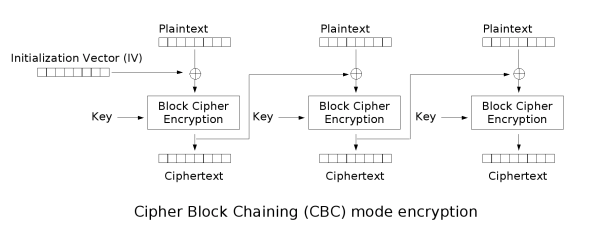
\includegraphics[width=.5\textwidth]{Cbc_encryption.png}
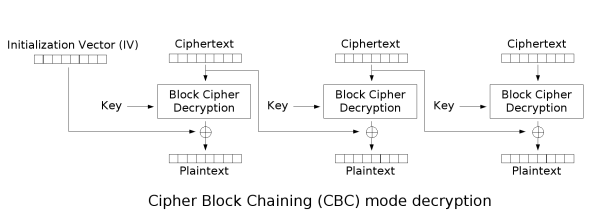
\includegraphics[width=.5\textwidth]{Cbc_decryption.png}
\end{center}
\caption{Data Flow in CBC Mode\protect\footnotemark}\label{fig:sd:cbc}
\end{figure}
\footnotetext{Images By WhiteTimberwolf (SVG version)---PNG version, Public Domain, \url{https://commons.wikimedia.org/w/index.php?curid=26434095} and \url{https://commons.wikimedia.org/w/index.php?curid=26434096}}


%\subsubsection{Feistel Ciphers}
%
%For this we can use a so called Feistel network.
%%Improving a comp. ind. encryption scheme to an ind. CPA secure scheme using a Feistel-network.
%\begin{definition}[A Feistel cipher]
% Let $k$ be any natural number (the number of \emph{rounds}). Let $f_{k_i}$ be a family of functions\protect\footnote{If possible pseudorandom functions and possibly one-way functions.} ($f$ is the so called \emph{round function}) of output length $n$ indexed by the sequence of \emph{round keys} $k_1, k_2, \ldots, k_n$. 
% Then the following encryption algorithm $E_k$ is called Feistel cipher. %network with $k$ iterations (for some odd $k$) based on a pseudo random generator $f_{k_i}$ and round keys $k_1, k_2, \ldots, k_n$ is an encryption scheme $(G,E,D)$, defined by:
% %For any odd $k\in\mathbb{N}$ we call an encryption scheme $(G, E, D)$ a Feistel network with $k$ iterations and $P$-Box $f$, iff for some \emph{round keys} $k_1, k_2, \ldots, k_n$ used as input for the pseudo random generator $f_{k_i}$. 
% \begin{itemize}
%  \item Fix a message $m=:x_1\circ x_2$, where $\left|x_1\right|=\left|x_2\right|=n$
%  \item Define the sequences $L_1, L_2, \ldots, L_n$ and $R_1, R_2, \ldots, R_n$ by $L_1:=x_1, R_1:=x_2$ and $L_{n+1}:=R_n, R_{n+1}:=L_n\oplus f_{k_n}(R_n)$. Finally define $E_k:x_1\circ x_2\to L_k\circ R_k$. 
% \end{itemize}
% Now we can define the corresponding decryption algorithm $D_k$ just like $e_k$, but with the reversed order of round keys:
% \begin{itemize}
%   \item Fix a ciphertext $c=:x_1\circ x_2$, where $\left|x_1\right|=\left|x_2\right|=n$
%   \item Define the sequences $L_1, L_2, \ldots, L_n$ and $R_1, R_2, \ldots, R_n$ by $L_1:=x_1, R_1:=x_2$ and $L_{n+1}:=R_n, R_{n+1}:=L_n\oplus f_{k_{k-n}}(R_n)$. Finally define $D_k:x_1\circ x_2\to L_k\circ R_k$. 
% \end{itemize}
%\end{definition}
%Feistel ciphers have been shown to fulfill several notions of security assuming that the round function is actually pseudo random. For instance Feistel networks with at least $3$ rounds are ind. CPA secure and for more rounds they fulfill even stronger notions of security. %  TODO: Check and clearify the exact model (3 seems sufficient under some assumptions, but 4 is definitely better (and already fulfills stronger notions)) and perhaps mention some other results. %see \url{https://link.springer.com/chapter/10.1007/978-3-540-45146-4\_30}

\subsubsection{Substitution-Permutation Networks}

A substitution-permutation network is a block cipher whose bijections arise as products of substitution and permutation ciphers.

To process a block of $N$ bits, the block is divided into $b$ chunks of $n=N/b$ bits each.
Each block is processed by a sequence of steps, each of which applies a bijection $B^N\to B^N$.

There are different kinds of steps:
\begin{itemize}
\item A \textbf{substitution step} consists of $b$ bijections $B^n\to B^n$, called \textbf{S-boxes}.
The substitution step maps each chunk by applying the corresponding S-box.

This expands on the ideas of polyalphabetic substitution ciphers from Sect.~\ref{sec:sd:crypto:hist}.
It substitutes each $n$-bit chunk by another chunk, and each chunk is substituted using a different substitution.

It is desirable to have every output bit of an S-box depend on \emph{every} input bit.
Then changing one input bit maximally \textbf{confuses} the output.

\item A \textbf{permutation step} consists of a permutation of $\{0,\ldots,N-1\}$, called a \textbf{P-box}.

The permutation step maps the entire block at once by permuting its bits according to the P-box.
This corresponds to a transposition cipher from Sect.~\ref{sec:sd:crypto:hist}.

It is desirable that the bits of one chunk are rearranged to as many different chunks as possible.
That maximizes the \textbf{diffusion} of bits among the chunks.

\item A \textbf{key step} consists of a number $k\in B^N$, called a \textbf{key}.
The key step maps a block by xor-ing it with $k$.

The key steps provide a way to parametrize the network.
We can use the same network multiple times by just switching to a different set of keys.
\end{itemize}

A \textbf{round} is a bijection of $B^N$ that is the product of some substitution and permutation steps and usually one key step.

A \textbf{network} is a sequence of rounds.
Often the substitution and permutation steps are the same for each round, and only the key of the key step changes between rounds.
In the simplest non-trivial case, the network consists of $b$ S-boxes (making up one substitution step), followed by one P-box, followed by one key step.
The more keys are available, the more rounds can be run, the more secure the network.

The inverse of a network is defined by inverting all operations in reverse order.

\begin{example}[Substitution-Permutation Network]\label{ex:sd:spn}
Fig.~\ref{fig:sd:subpernet} shows a Substitution-Permutation Network.
It uses $N=16$ and $b=n=4$.
Its rounds consists of one substitution step (using $4$ S-boxes), one permutation step (using P-box $P$), and one key step.

$4$ rounds are concatenated using keys $K_0,\ldots,K_3$ that are obtained from one overall key.
The first round only uses the key step, and the last round skips the permutation step.
\end{example}

\begin{figure}[htb]
\begin{center}
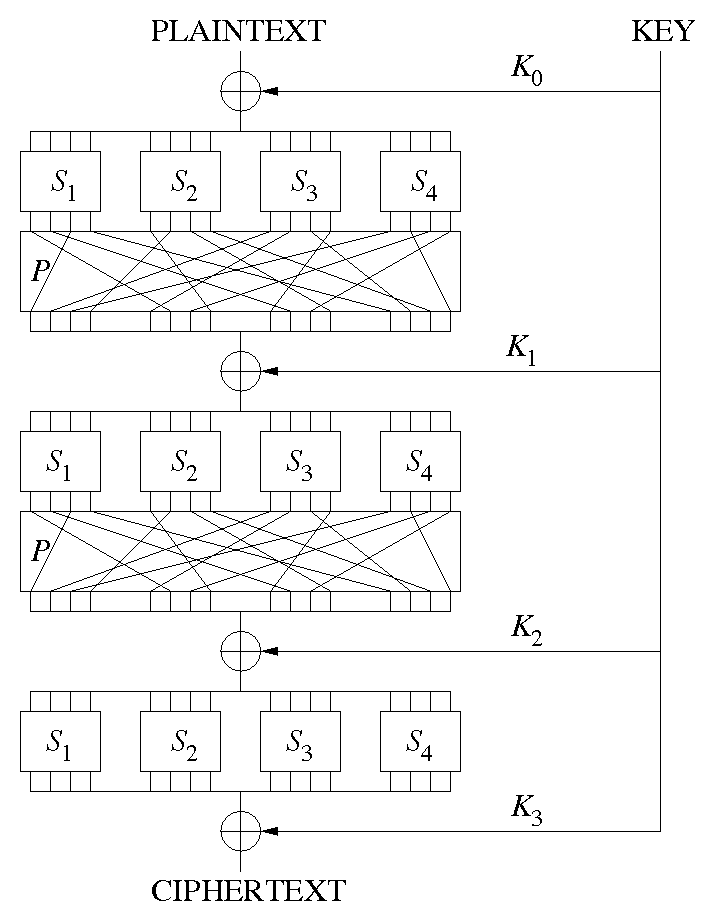
\includegraphics[width=.5\textwidth]{SubstitutionPermutationNetwork.png}
\end{center}
\caption{A simple Substitution-Permutation-Network\protect\footnotemark}\label{fig:sd:subpernet}
\end{figure}
\footnotetext{Image by GaborPete---Own work, CC BY-SA 3.0, \url{https://commons.wikimedia.org/w/index.php?curid=6420152}}

\begin{exercise}\label{exc:sd:spn}
Consider the network for $N=8$ and $b=2$, whose rounds consist of the following steps:
\begin{compactenum}
 \item Substitution step consisting of the S-box $S=S_1=S_2$.
  The substitution $S:B^4\to B^4$ is given by $x\longmapsto ((x+1)\cdot 7)\modop 17-1$.
  This is a bijection of $B^4$, where $4$-bit chunks are seen as natural numbers via their binary encoding.
 \item Permutation step consisting of the P-box $P:B^8\to B^8$, which does a cyclic $2$-bit left-shift of its argument.
 \item Key step with $8$-bit key $k_i$ where $i$ is the number of the round.
\end{compactenum}
The network consists of two rounds using a $16$-bit key $k$, whose first $8$ bits are $k_1$ and whose last $8$ bits are $k_2$.

We obtain an encryption scheme by using CBC mode with an IV that is generated randomly.

Assume the key is $1001\,1000\,0010\,0110$.

Manually encrypt the plaintext \texttt{abc} (seen as $3$ blocks of $8$ bits using ASCII encoding), assuming the IV is $1010\,1010$.

Decrypt the ciphertext again.
\end{exercise}


%Substitution-permutation-network and Feistel networks using $S$-Boxes are quite similar.
%Ciphers based on substitution-permutation-networks can be better parallelized, but Feistel ciphers can use any pseudo-random function (for instance any one-way function) and are therefore limited to invertible ($P$-Boxes). %Also the Feistel networks can be adapted to ciphers not using blocks (for instance it is used in OAEP).

\subsubsection{AES}

% https://www.tutorialspoint.com/cryptography/images/aes_structure.jpg

\paragraph{Overview}
AES (Advanced Encryption Standard) was chosen by NIST (the US institute of standards and technology) in 2001 as an encryption standard after an open call in 1997 and extensive analysis of the submitted schemes.
Before being adopted as AES, it was called Rijndael.
It replaced DES, which was not secure anymore.

AES is one of the most widely used block ciphers, approved by many government organizations.
Implementations are available in many programming languages.

AES uses a substitution-permutation network for $N=128$, $b=16$, and $n=8$.

\paragraph{Keys}
While Rijndael is very flexible, NIST chose only three special cases for AES.
They differ mainly by the key size and the number of rounds:
\begin{center}
  \begin{tabular}{|c|c|c|c|}
  	\hline key size & 128-bit & 192-bit & 256-bit \\ 
  	\hline number of rounds & 10 & 12 & 14 \\ 
  	\hline
  \end{tabular}
\end{center}
In all three cases, one additional initial round is run that only xors the input with a round key.

Thus, $11$, $13$, or $15$ $128$-bit round keys $k_0,\ldots,k_r$ for $r\in\{10,12,14\}$ are needed.
These are obtained from the overall key using the Rijndael key schedule, which we omit here.

\paragraph{Details}
The substitution-permutation network of AES looks as follows:
\begin{compactenum}
 \item Round 0: key step with $k_0$
 \item Round $i$ for $i=1,\ldots,r-1$:
  \begin{compactenum}
    \item substitution step (called \emph{sub-bytes}) with a fixed $8$-bit S-box used $16$ times
    \item permutation step (called \emph{shift-row}) with a fixed permutation of $128$ bits
    \item substitution step (called \emph{mix-columns}) with a fixed $32$-bit S-box used $4$ times
    \item key step (called \emph{add-round-key}) with key $k_i$
  \end{compactenum}
 \item Round $r$: as before but without the mix-columns step
\end{compactenum}

The $128$-bit block to be mapped is represented as $16$ chunks of $8$ bits.
The chunks are arranged as a $4\times 4$ matrix.
The $4$ basic steps are defined as follows:
\begin{compactitem}
  \item sub-bytes: This substitution step applies a fixed S-box (the Rijndael S-box, which we omit here) to every chunk.
  \item shift-row: This permutation step leaves the chunks as they are but rearranges them relative to each other.
    Specifically, for $i=0,1,2,3$, the $i$-th row of the matrix is left-shifted cyclically $i$ times.
  \item mix-columns: This is a more complex step that applies the same fixed substitution to each column of the matrix.
    Thus, this step can be seen as a substitution step using $4$ chunks of size $32$, and using the same fixed S-box $4$ times.
    
    The fixed S-box is defined as follows.
    A column consists of $4$ bytes, each of which can be seen as an element of $F_{2^8}$ (see Sect.~\ref{sec:math:finfield} for finite fields).
    Thus, a column of $32$ bits can be seen as a $4$-dimensional vector over $F_{2^8}$.
    This vector is multiplied with the fixed $4\times 4$ matrix over $F_{2^8}$ given by
    \[\left(\begin{matrix}
    2&3&1&1\\1&2&3&1\\1&1&2&3\\3&1&1&2
   \end{matrix}\right)\]
  \item add-round-key: This key steps xors all $128$ with the respective round key.
\end{compactitem}


\section{Asymmetric Encryption}\label{sec:sd:crypto:asym}
The basic idea of asymmetric encryption is that different keys are used for encryption and decryption.
An important requirement for security is that the decryption key cannot be computed from the encryption key.

This has the practical advantage that the---not security-critical---encryption key can be made public.

\subsection{Schemes}

We only need to make a minor modification to the Def.~\ref{def:sd:symscheme}:

\begin{definition}[Asymmetric Encryption Scheme]\label{def:sd:asymscheme}
 An \textbf{asymmetric encryption scheme} is an encryption scheme $(\Sigma,K, G, E, D)$, where
  \begin{compactitem}
   \item $K_n=K^e_n\times K^d_n$
   \item if $k=(k^e,k^d)$, then $E_k$ depends only on $k^e$ and $D_k$ depends only $k^d$
  \end{compactitem}
\end{definition}
Intuitively, the keys are pairs of an encryption and a decryption key.

\subsection{Schemes based on Modular Arithmetic}

We fix the alphabet to be $\Sigma=\{0,1\}$ and identify the elements of $\Sigma^n$ and with natural numbers in binary representation.

\subsubsection{Modular Arithmetic as a Cipher}

To encrypt plaintexts from $\Sigma^n$, we proceed in two steps:
\begin{compactenum}
 \item We embed the plaintext into $\Z_N$ for certain $N>2^n$.
 \item We apply a cipher function $\Z_N\to\Z_N$.
\end{compactenum}

$N$ is part of the key.
The number of bits in $N$ is usually seen as the size of the key.
This size must be greater than $n$.

The embedding introduces randomness to make sure that encrypting the same plaintext multiple times yields different ciphertexts.
The cipher function is the main source of security.

\subsubsection{Mode of Operation and Padding}

\paragraph{No Mode of Operation}
In principle, we could use the same modes of operation as for block ciphers.
However, that is not common:
\begin{compactitem}
 \item Asymmetric encryption has the advantage that the encryption key can be made public.
 To exploit that advantage, it is practical not to change the key very often.
 In that case, using the same key for many blocks of many long message increases the chance of attacks.
 \item Asymmetric encryption tends to be more complex than symmetric encryption.
 Therefore, it is not practical to use asymmetric encryption for many long messages.
\end{compactitem}
Instead, it makes more sense to use \textbf{hybrid encryption}: use an asymmetric scheme only to transmit the key for a symmetric scheme.
In that case, it is not necessary to be able to send arbitrarily long messages with the same fixed key.
Instead, a fixed message length suffices as long as it can hold the symmetric key.

\paragraph{Padding}
For the same reason as with symmetric schemes, some randomness must be introduced into the encryption function to make sure that repeatedly mapping the same plaintext yields different ciphertexts.
That is the role of the \textbf{padding}, which embeds the plaintext from $\Z_{2^n}$ into $\Z_N$.

The basic idea is to pick $N>2^{n+i}$, append $i$ $0$s to the plaintext and then apply some cipher $\Z_{2^{n+i}}\to\Z_{2^{n+1}}$ (e.g., a substitution-permutation network with a randomly chosen parameter).

The details of padding are very difficult and subject to active research.
The most important example is Optimal Asymmetric Encryption Padding (OAEP).
Multiple padding schemes based on OAEP have been standardized in RFC 447: Public-Key Cryptography Standards (PKCS) \#1.

\subsubsection{RSA}

\paragraph{Overview}
RSA is a family of cipher functions based on modular arithmetic.

It was developed in the 1970s inspired by ideas by Diffie and Hellman.
It is named after the authors of the algorithm (Rivest, Shamir, Adleman).
A related algorithm was developed earlier by the UK secrete service but remained classified until the 1990s.

The basic ideas is to use $N=p\cdot q$ for large prime numbers $p$ and $q$.
Becuase it is (assumed to be) very difficult to compute $p$ and $q$ from $N$, $p$ and $q$ remain private even if $N$ is public.

\paragraph{Key Generation}
To compute $G(n)$, we first randomly choose two large primes $p$ and $q$ (typically of roughly equal size) such that $p\cdot q>2^{n+i}$ where $i$ is the desired number of padding bits.
We put $N=p\cdot q$.

Secondly, we put $m=(p-1)(q-1)$. (Actually, any common multiple of $p-1$ and $q-1$ is fine.)
Note that $m=\phi(N)$.
Then we pick $e\in \Z_m$ such that $\gcd(e,m)=1$ and compute the $d\in\Z_m$ with $e\cdot d\Equiv_m 1$.
Such a $d$ exists because $\gcd(e,m)=1$ and is easy to compute (see Thm.~\ref{thm:math:extendedeuclid}).

The keys are now defined as follows:
\begin{compactitem}
 \item public key (encryption key): $(N,e)$
 \item private key (decryption key): $(N,d)$
\end{compactitem}
$m$, $p$, and $q$ are not needed for encryption or decryption but must remain private: $p$ (or $q$) is enough to compute $m$ from $N$, and $m$ is enough to compute $d$ from $e$.
So we delete $m$, $p$, and $q$ after generating the key.

Note that to choose $p$ and $q$ efficiently, it is important to have access to a fast primality test.

\paragraph{Encryption and Decryption}
The cipher function and its inverse are the functions $\Z_N\to \Z_N$ defined by
\begin{compactitem}
 \item encryption: $x\mapsto x^e\modop N$
 \item decryption: $x\mapsto x^d\modop N$
\end{compactitem}

Both can be computed efficiently, e.g., using square-and-multiply.

These are indeed inverse to each other:

\begin{theorem}
For all $x\in \Z_N$, we have $(x^d)^e\Equiv_N (x^e)^d \Equiv_N x$.
\end{theorem}
\begin{proof}
In general, because $N=p\cdot q$ for prime numbers $p$ and $q$, we have that $x\Equiv_N y$ iff $x\Equiv_p y$ and $x\Equiv_q y$.

So we have to show that $x^{de}\Equiv_p x$.
(We also have to show the same result for $q$, but the proof is the same.)
We distinguish two cases:
\begin{compactitem}
\item $p|x$: Then trivially $x^{de}\Equiv_p 0\Equiv_p x$.
\item Otherwise. Then $p$ and $x$ are coprime.\\
   By construction of $e$ and $d$ and using Thm.~\ref{thm:math:extendedeuclid}, we have $k\in\Z$ such that $e\cdot d+k\cdot m=1$.
   Using $m=(p-1)(q-1)$, we obtain $x^{de}=x\cdot (x^{p-1})^{-k\cdot(q-1)}$.
   That yields $x^{de}\Equiv_p x$ by using $x^{p-1}\Equiv_p 1$ as known from Thm.~\ref{thm:math:fermatlittle}.
\end{compactitem}
\end{proof}

\paragraph{Attacks}
To break RSA, $d$ has to be computed.
There are $3$ natural ways to do that:
\begin{compactitem}
 \item Factor $N$ into $p$ and $q$. Then compute $d$ easily.
 \item Compute $m$ using $m=\phi(N)$ (which may be easier than finding $p$ and $q$). Then compute $d$ easily.
 \item Find $d$ such that $e\cdot d\Equiv_m 1$ (which may be easier than finding $m$).
\end{compactitem}
Currently these are believed to be equally hard.

It is believed that there is no algorithm for factoring $N$ that is polynomial in the number of bits of $N$.
That is not proved.
There are hypothetical machines (e.g., quantum computers) that can factor $N$ polynomially.

Note that checking if $N$ can be factored (without producing the factors) is polynomial, and practical algorithms exist (in particular, the AKS algorithm).
Incidentally, that is important to find the large prime number $p$ and $q$ efficiently.
\medskip

If there is indeed no polynomial algorithm, factoring relies on brute-force attacks that find all prime numbers $k<\sqrt{N}$ and test $k|N$.
Therefore, larger keys are harder than break to smaller ones.
Because of improving hardware, the key size that is considered secure grows over time.

Keys of size $1024$ are considered secure today, but because security is a relative term, keys of size $2048$ are often recommended. 
%It is quetionable that 1024-bit rsa is really secure, even though it has not yet been publicly broken;
%(see for instance https://en.wikipedia.org/wiki/RSA_%28cryptosystem%29#Integer_factorization_and_RSA_problem or https: //www.schneier.com/blog/archives/2007/05/307digit_number.html).
Larger keys are especially important if data is needed to remain secure far into the future, when faster hardware will be available.


\section{Hashing}\label{sec:sd:crypto:hash}
This topic was covered in a presentation by a student.

\section{Authentication}\label{sec:sd:crypto:auth}
\subsection{Using Asymmetric Encryption}

An important application of asymmetric encryption is authentication.

For example, an agent $A$ who wants to prove her identity can generate a key and publish the public key.
To authenticate $A$, we generate a random string, encrypt it with the public key, and ask for its decryption.
Because only $A$ can decrypt, this is sufficient to authenticate.

Another authentication scheme uses a digital signature.
Here the private key is used for encryption and the public one for decryption. (Note that for RSA the distinction between encryption and decryption key is insubstantial anyway.)
$A$ sends a message together with its encryption, and the recipient decrypts and compares.
A better scheme arises if $A$ first applies a cryptographic hash to the message and sends the original message and the encrypted hash value.

\subsection{Multi-Factor Authentication}

The idea of multi-factor authentication is to use the conjunction of multiple authentication tests.
This is particularly useful if two factors are used that depend on fundamentally different systems: in that case authentication is still safe even if one of the systems is compromised.

The most common application is to authenticate a user via password first, then ask for a second one-time password.
Usually the one-time password is sent to the user as a text message or (in older systems) as a list of one-time passwords on paper by mail.
Even if the user's password is compromised, the authentication remains secure (and can be used to reset the original password).
However, to be truly secure, the user must never type his password on the phone.

%\section{Key Generation and Distribution}
   % security protocol correctness, such as key management protocol correctness,
   % e.g., going back to the work by Burrows, Abadi, and Needham on a logic of authentication (https://doi.org/10.1145/77648.77649)
   % Its an application of logic to a concrete problem space where errors are obviously bad.


   % database security -> peter
   % network security: see also Jürgen Schönwälder, slides 269-324

  \chapter{Privacy}\label{sec:sd:privacy}
   This topic was covered in a presentation by a student.
   
   % differential privacy: see also wikipedia or http://www.cis.upenn.edu/~aaroth/courses/privacyF11.html

%\part{Summary}
%
%\chapter{}
%  \input{summary}

\part{Appendix}

\appendix

\chapter{Mathematical Preliminaries}\label{sec:math}
\input{../math/all}

\chapter{Solutions to Selected Exercises}
\begin{exsolution}{exc:sd:viginere}
$\phi_k(i,x)=(x+k_{i\modop l})\modop n$.
\end{exsolution}

\begin{exsolution}{exc:sd:railfence}
Let $f=l/k$ be the length of the fence.
Then $\tau_k(i) = (i\modop k)\cdot f + (i\divop k)$.
Its inverse is $\tau_k^{-1}(j)=(j\modop f)\cdot k + (j\divop f)$.
\end{exsolution}

\tocentryBib

\input{\currfilebase.bblp}
%\bibliographystyle{alpha}
%\bibliography{securitySources}
%\bibliography{../../../../../Program_Data/Latex/bib/rabe,../../../../../Program_Data/Latex/bib/systems,../../../../../Program_Data/Latex/bib/historical}

\end{document}
